
\chapter{Evaluaci\'on del algoritmo propuesto y resultados}

En este cap\'itulo se presenta la evaluaci\'on experimental del algoritmo desarrollado en este trabajo de tesis. 
La evaluaci\'on se realiz\'o utilizando un conjunto diverso de problemas multi-objetivo que reunen diferentes caracter\'isticas que causan 
dificultades a un algoritmo evolutivo multi-objetivo. El estudio experimental descrito en este cap\'itulo est\'a dividido 
en tres partes: la primera parte muestra los resultados para el conjunto de problemas ZDT (\textit{Zitzler-Deb-Thiele}), 
la segunda muestra los resultados para el conjunto de problemas de DTLZ (\textit{deb-Thiele-Laumanns-Zitzler}). 
Finalmente, la tercera y \'ultima parte muestra los resultados de escalabilidad. Los resultados se contrastan 
con las soluciones obtenidas por los algoritmos NSGA-II (\textit{the Nondominated Sorting Genetic Algoritm -II}), SMS-EMOA 
(\textit{Multi-objective Selection based on Dominated Hypervolume}) y MOPSOcd (\textit{Multi-objective Particle Swarm Optimizer based on 
Crowding Distance}).
  
  \section*{Par\'ametros}
  
  Los par\'ametros utilizados para los algoritmos MOPSOhv y MOPSOcd se muentran en la tabla \ref{tab:parametros1}. Se us\'o un factor de 
  inercia $\omega = 0.4$ y constantes sociales $\varphi_{1}=\varphi_{2}=1$.
 
 \begin{table}[H]
  \begin{center}
    \begin{tabular}{|l||c|c|c|}
	\hline
	& \textbf{Generaciones}  & \textbf{Poblaci\'on} & \textbf{Mutaci\'on} \\
	\hline
	\hline
	\textbf{MOPSOhv} & 1200 & 100 &0.5\\ 
	\hline
	\textbf{MOPSOcd} & 1200 & 100 &0.5\\
	\hline
	\end{tabular}
	\caption{Par\'ametros para los algoritmos de c\'umulos de part\'iculas}
  \label{tab:parametros1}
  \end{center}
\end{table}

Los par\'ametros utilizados para el NSGA-II se muestran en la tabla \ref{tab:parametros2}. Los par\'ametros
utlizados para el SMS-EMOA se muestran en la tabla \ref{tab:parametros3}.

\begin{minipage}{0.5\textwidth}
\begin{table}[H]
  \begin{center}
    \begin{tabular}{|l||c|c}
	\hline
	Generaciones  & 1200 \\ 
	\hline
	Poblaci\'on & 100 \\ 
	\hline
	Cruza & 0.9 \\
	\hline
	Mutaci\'on & 0.01 \\
	\hline
  \end{tabular}
  \caption{Par\'ametros de NSGA-II}
  \label{tab:parametros2}
\end{center}
\end{table}
\end{minipage}
\begin{minipage}{0.5\textwidth}
\begin{table}[H]
	\begin{center}
		\begin{tabular}{|l||c|c}
			\hline
			Generaciones  & 3000 \\ 
			\hline
			Poblaci\'on & 100 \\ 
			\hline
			$\eta_c = \eta_m$ & 20 \\ 
			\hline
			Mutaci\'on & 0.033\\ 
			\hline			
		\end{tabular}
		\caption{Par\'ametros de SMS-EMOA}
		\label{tab:parametros3}
	\end{center}
\end{table}
\end{minipage}

El uso de una sola m\'etrica dif\'icilmente puede reflejar el desempe\~no global de un algoritmo evolutivo multi-objetivo. Algunas
m\'etricas miden la convergencia del algoritmo al frente de Pareto real, otras la distribuci\'on y la diversidad de las soluciones. 
En este caso necesitamos evaluarlo considerando varias m\'etricas simult\'aneamente. Sin embargo, la m\'etricas evalu\'an dos 
objetivos en conflicto (la convergencia y la diversidad). Si los valores de las m\'etricas de un algoritmo dominan a las de otro,
entonces podemos afirmar que el primero es mejor que el segundo. En otro caso, no podemos concluir nada acerca de los dos algoritmos.
Las m\'etricas que se utilizar\'an para evaluar la eficacia son el espaciamiento para evaluar la distribuci\'on; y la distancia generacional 
invertida, la cobertura de dos conjuntos y el indicador del hipervolumen para evaluar la convergencia.


\section{Conjunto de problemas ZDT}

Estos problemas est\'an dise\~nados poniendo \'enfasis en algunas de las caracter\'isticas que causan dificultades para un algoritmo 
evolutivo multi-objetivo. Estos problemas tienen una misma estructura y consisten de tres funciones, $F$, $g$ y $h$, se describe a 
continuaci\'on \cite{Zitzler2000}:

\begin{align*}
\text{Minimizar}\hspace{0.5cm} F&=(f_1(x_1),f_2(x_2))\\
\text{Sujeto a }\hspace{0.5cm} f_2(x)&=g(x_2,\ldots,x_m)\cdot h(f_1(x_1),g(x_2,\ldots,x_m)),\\
\text{donde}\hspace{0.5cm} x&= (x_1,\ldots, x_m)
\end{align*}

La funcion $f_1$ depende solamente de la primera variable de decisi\'on, $g$ es una funci\'on de las
$m-1$ variables restantes, y los par\'ametros de $h$ son los valores de las funciones $f_1$ y $g$.

\begin{itemize}
 
\item La funci\'on de prueba \textbf{ZDT1} tiene un frente de Pareto convexo:
\begin{align*}
f_1(x)&=x_1\\
f_2(x,g(x))&=g(x)\cdot\left(1-\sqrt{ \frac{f_1}{g(x)}}\right)\\
g(x)&=1+\frac{9}{n-1}\cdot\sum_{i=2}^nx_i
\end{align*}
donde $n=30$ y $x_i\in[0,1]$ con $i=1,\ldots, n$. El frente de Pareto real se forma con $g(x)=1$ (figura \ref{fig:zdt1}).

\item La funci\'on de prueba \textbf{ZDT2} tiene un frente de Pareto c\'oncavo:

\begin{align*}
f_1(x)&=x_1\\
f_2(x,g(x))&=g(x)\cdot(1- \left( \frac{f_1}{g(x)}\right)^2)\\
g(x)&=1+\frac{9}{n-1}\cdot\sum_{i=2}^nx_i
\end{align*}
donde $n=30$ y $x_i\in[0,1]$ con $i=1,\ldots, n$. El frente de Pareto real se forma con $g(x)=1$ (figura \ref{fig:zdt2}).

\item La funci\'on de prueba \textbf{ZDT3} tiene un frente de Pareto discontinuo y convexo:

\begin{align*}
f_1(x)&=x_1,\\
f_2(x,g)&=g(x)\cdot\left(1-\sqrt{\frac{f_1(x)}{g(x)}}-\frac{f_1(x)}{g(x)}\sin(10\cdot\pi\cdot f_1(x))\right)\\
g(x)&=1+\frac{9}{n-1}\cdot\sum_{i=2}^nx_i
\end{align*}
donde $n=30$ y $x_i\in[0,1]$ con $i=1,\ldots, n$. El frente de Pareto real se forma con $g(x)=1$. La funci\'on seno
en $h$ produce una discontinuidad en el frente de Pareto. Sin embargo, no hay discontinuidad en el espacio de las variables 
de decisi\'on (figura \ref{fig:zdt3}).

\item La funci\'on de prueba \textbf{ZDT4} tiene $21^9$ frentes locales, lo que pone a prueba la habilidad de un 
algoritmo para lidiar con problemas multifrontales:

\begin{align*}
f_1(x)&=x_1,\\
f_2(x,g(x))&=g(x)\cdot \left(1-\sqrt{ \frac{f_1(x)}{g(x)}}\right),\\
g(x)&=1+10\cdot(n-1)+ \sum_{i=2}^n(x_i^2-10\cdot \cos(4\cdot\pi\cdot x_i))
\end{align*}

donde $n=10$, $x_1\in[0,1]$ y $x_i \in[-5,5] $ con $i=2, \ldots, n$. El frente de Pareto real se forma con $g(x)=1$ (figura \ref{fig:zdt4}).

\item La funci\'on de prueba \textbf{ZDT6} tiene un espacio de b\'usqueda no uniforme:

\begin{align*}
f_1(x)&=1- e^{(-4\cdot x_1)} \cdot \sin^6(6\cdot\pi\cdot x_1),\\
f_2(x,g(x))&=g(x)\cdot(1-\left(\frac{f_1}{g(x)}\right)^2),\\
g(x)&=1+9\cdot\left[\frac{\sum_{i=2}^n}{9}\right]^{0.25}
\end{align*}

donde $n=10$, $x_1\in[0,1]$ y $x_i \in[-5,5]$ con $i= 2, \ldots, n$. El frente de Pareto real se forma con $g(x)=1$.
Este problema tiene una baja densidad en las soluciones cerca del frente de Pareto real y una alta densidad lejos del mismo (figura \ref{fig:zdt6}).

\end{itemize}

\begin{figure}
\centering
    \centering
    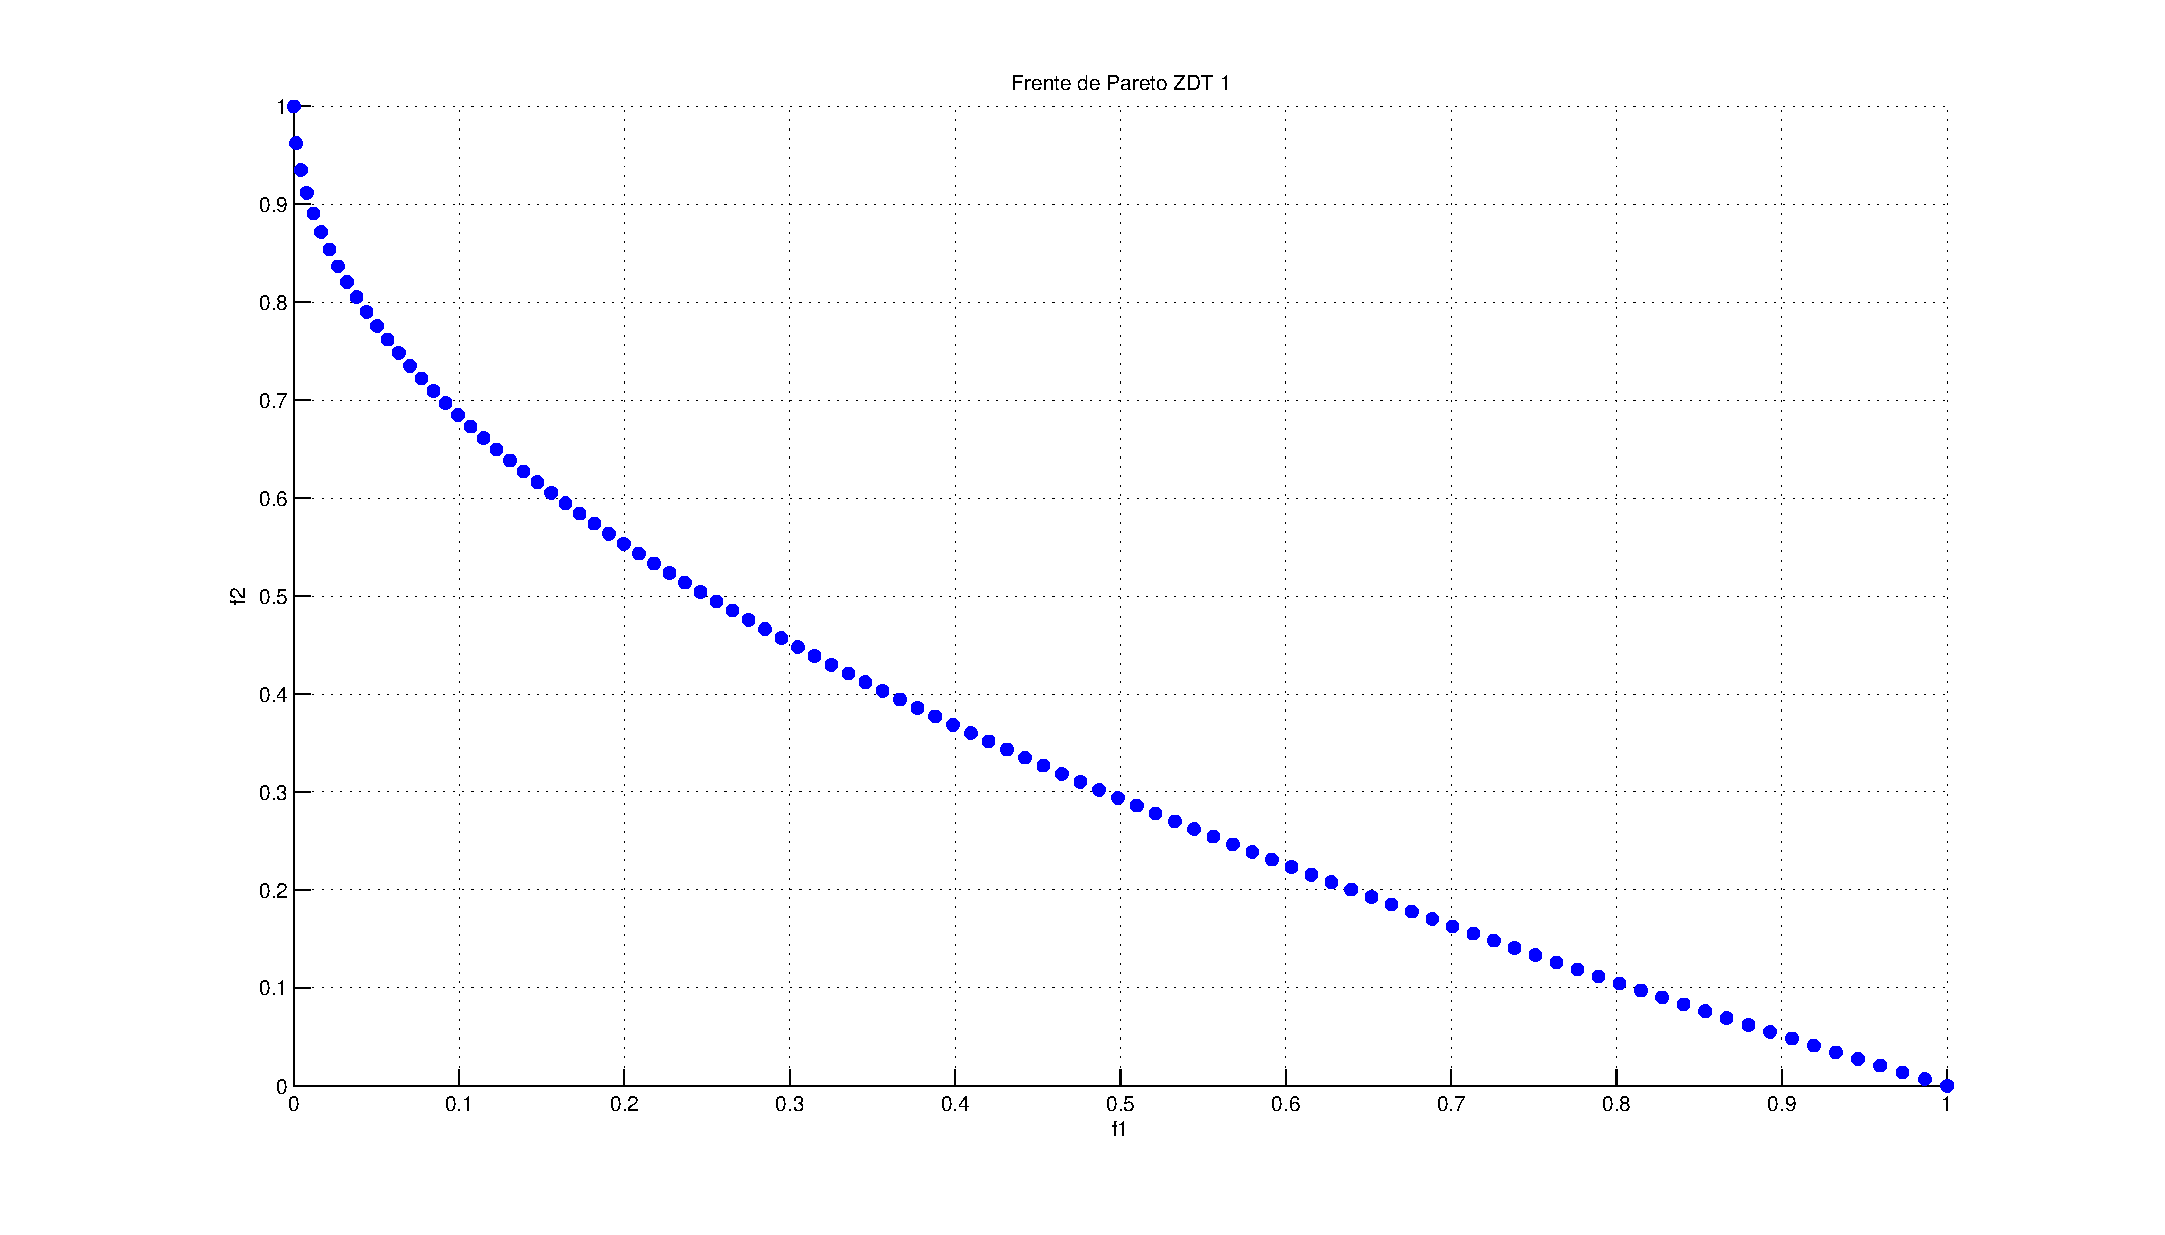
\includegraphics[scale=0.4]{ApendiceA/paretoZDT1.eps}
    \caption{Frente de Pareto verdadero de ZDT1}
    \label{fig:zdt1}
\end{figure}
 
\begin{figure}
\centering
 
    \centering
    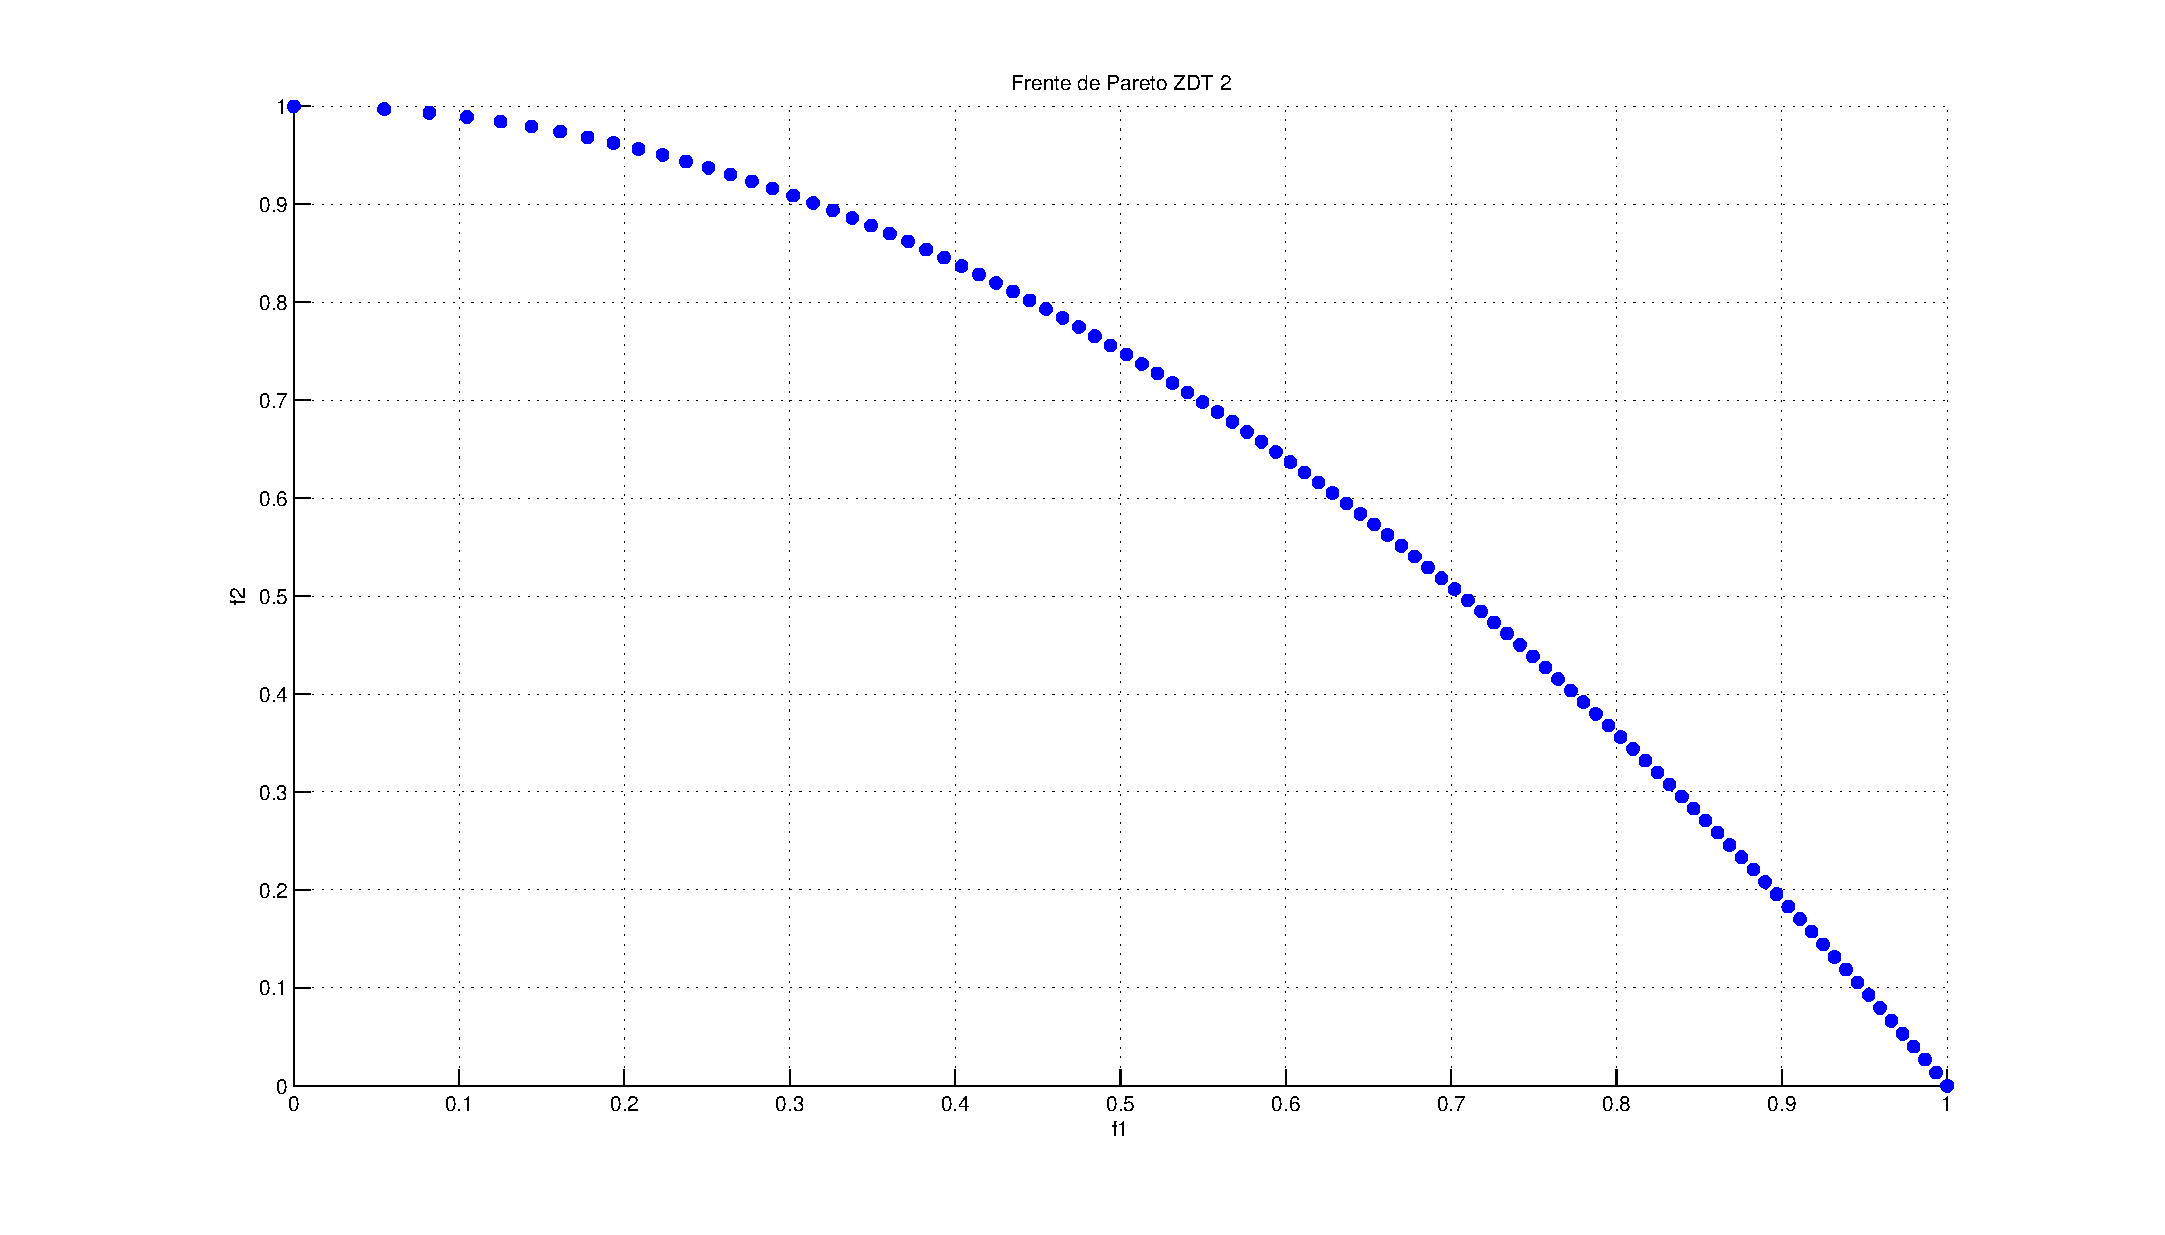
\includegraphics[scale=0.4]{ApendiceA/paretoZDT2.eps}
    \caption{Frente de Pareto verdadero de ZDT2}
    \label{fig:zdt2}
\end{figure}

\begin{figure}
\centering
    \centering
    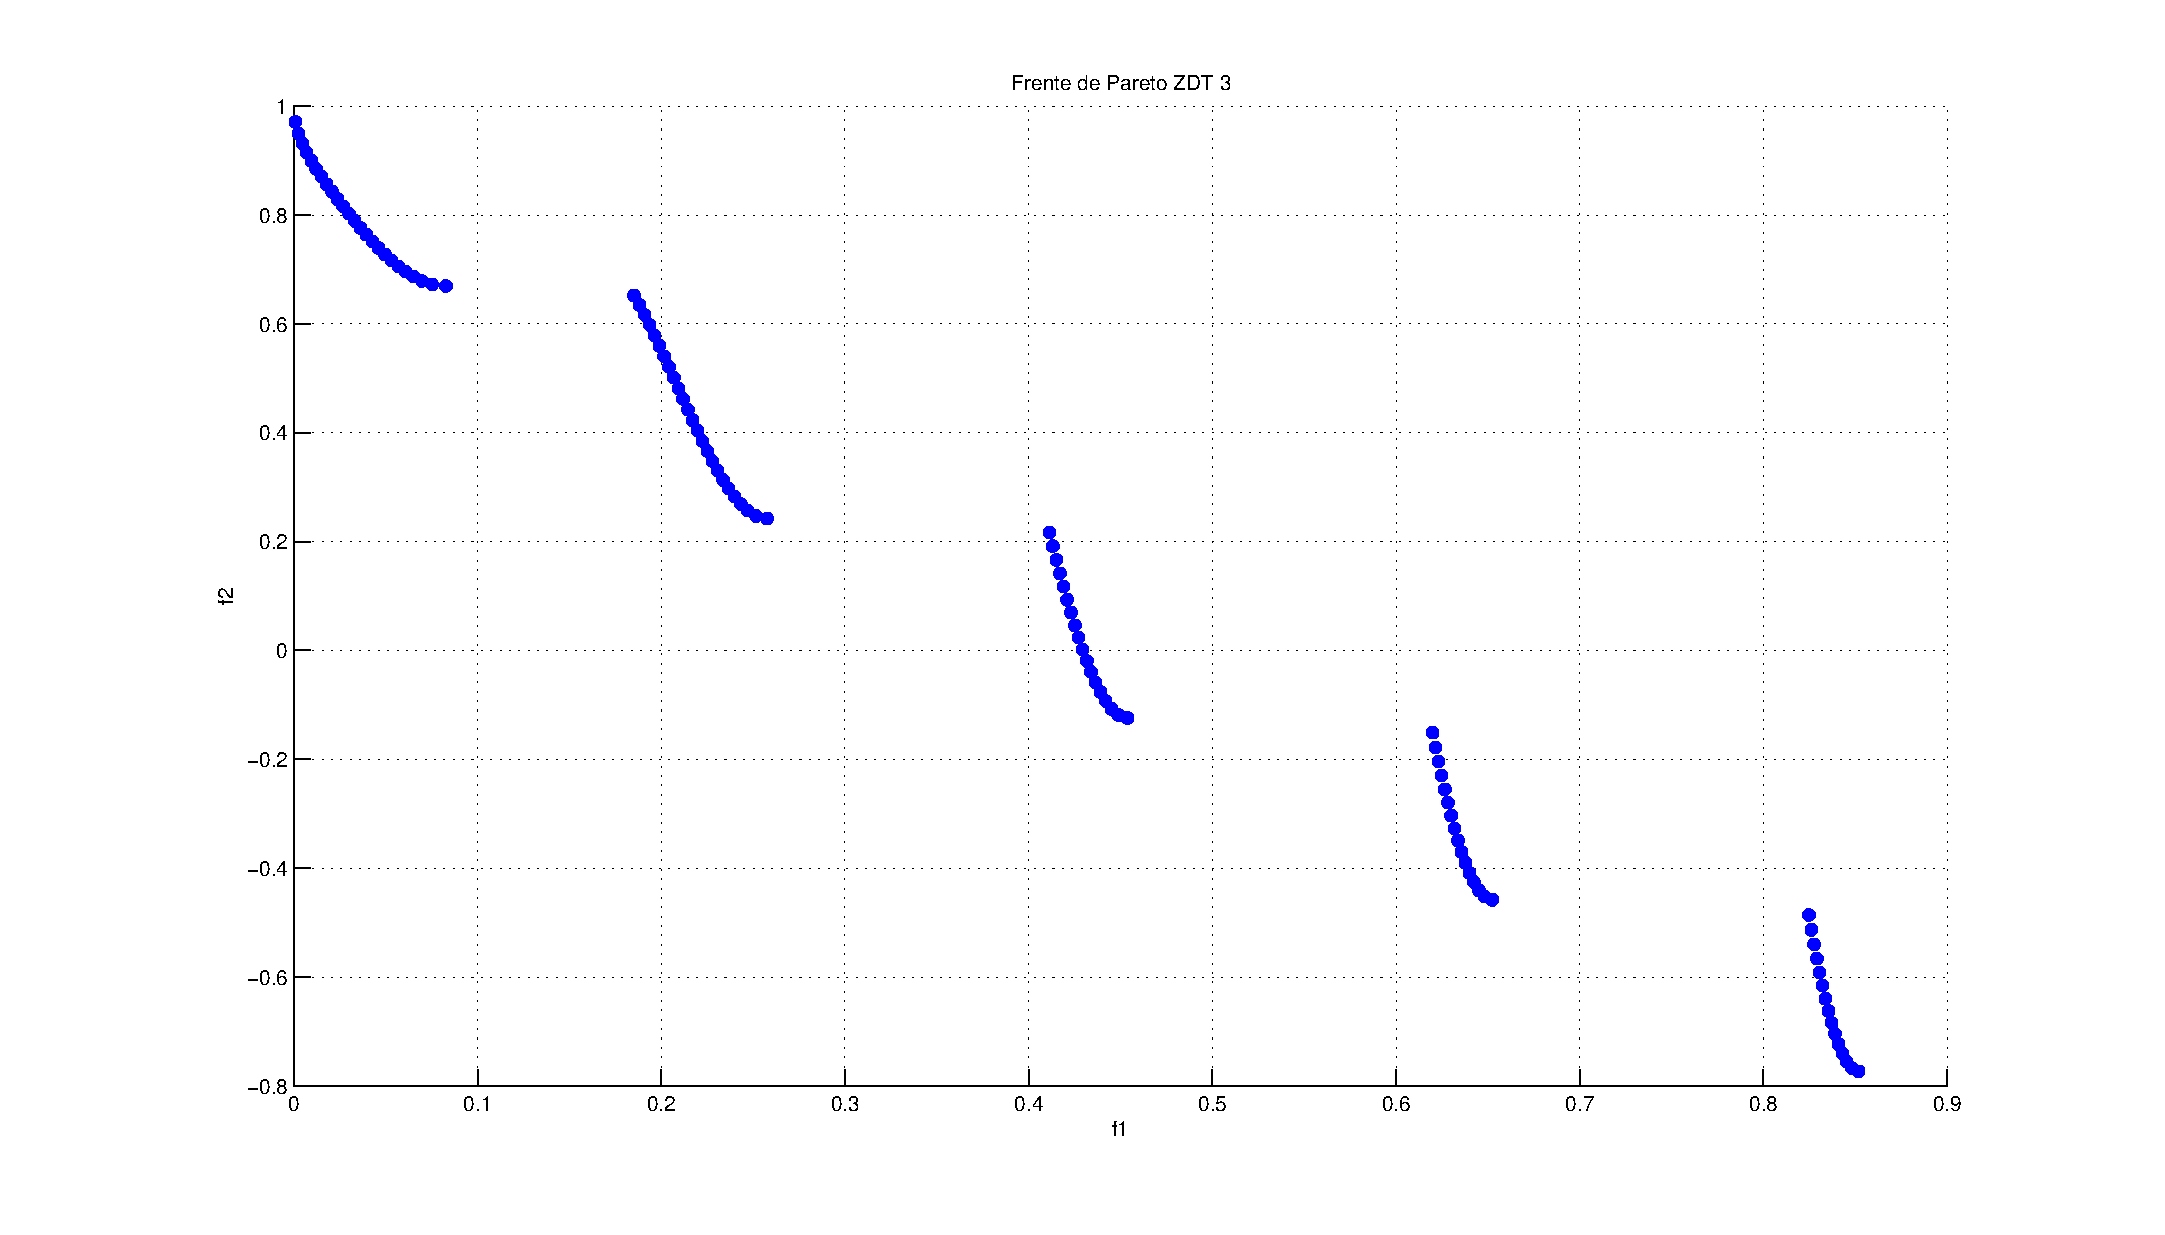
\includegraphics[scale=0.4]{ApendiceA/paretoZDT3.eps}
    \caption{Frente de Pareto verdadero de ZDT3}
    \label{fig:zdt3}
\end{figure}

\begin{figure}
\centering
    \centering
    \includegraphics[scale=0.4]{ApendiceA/paretoZDT4.eps}
    \caption{Frente de Pareto verdadero de ZDT4}
    \label{fig:zdt4}
\end{figure}
\begin{figure}
\centering
    \centering
    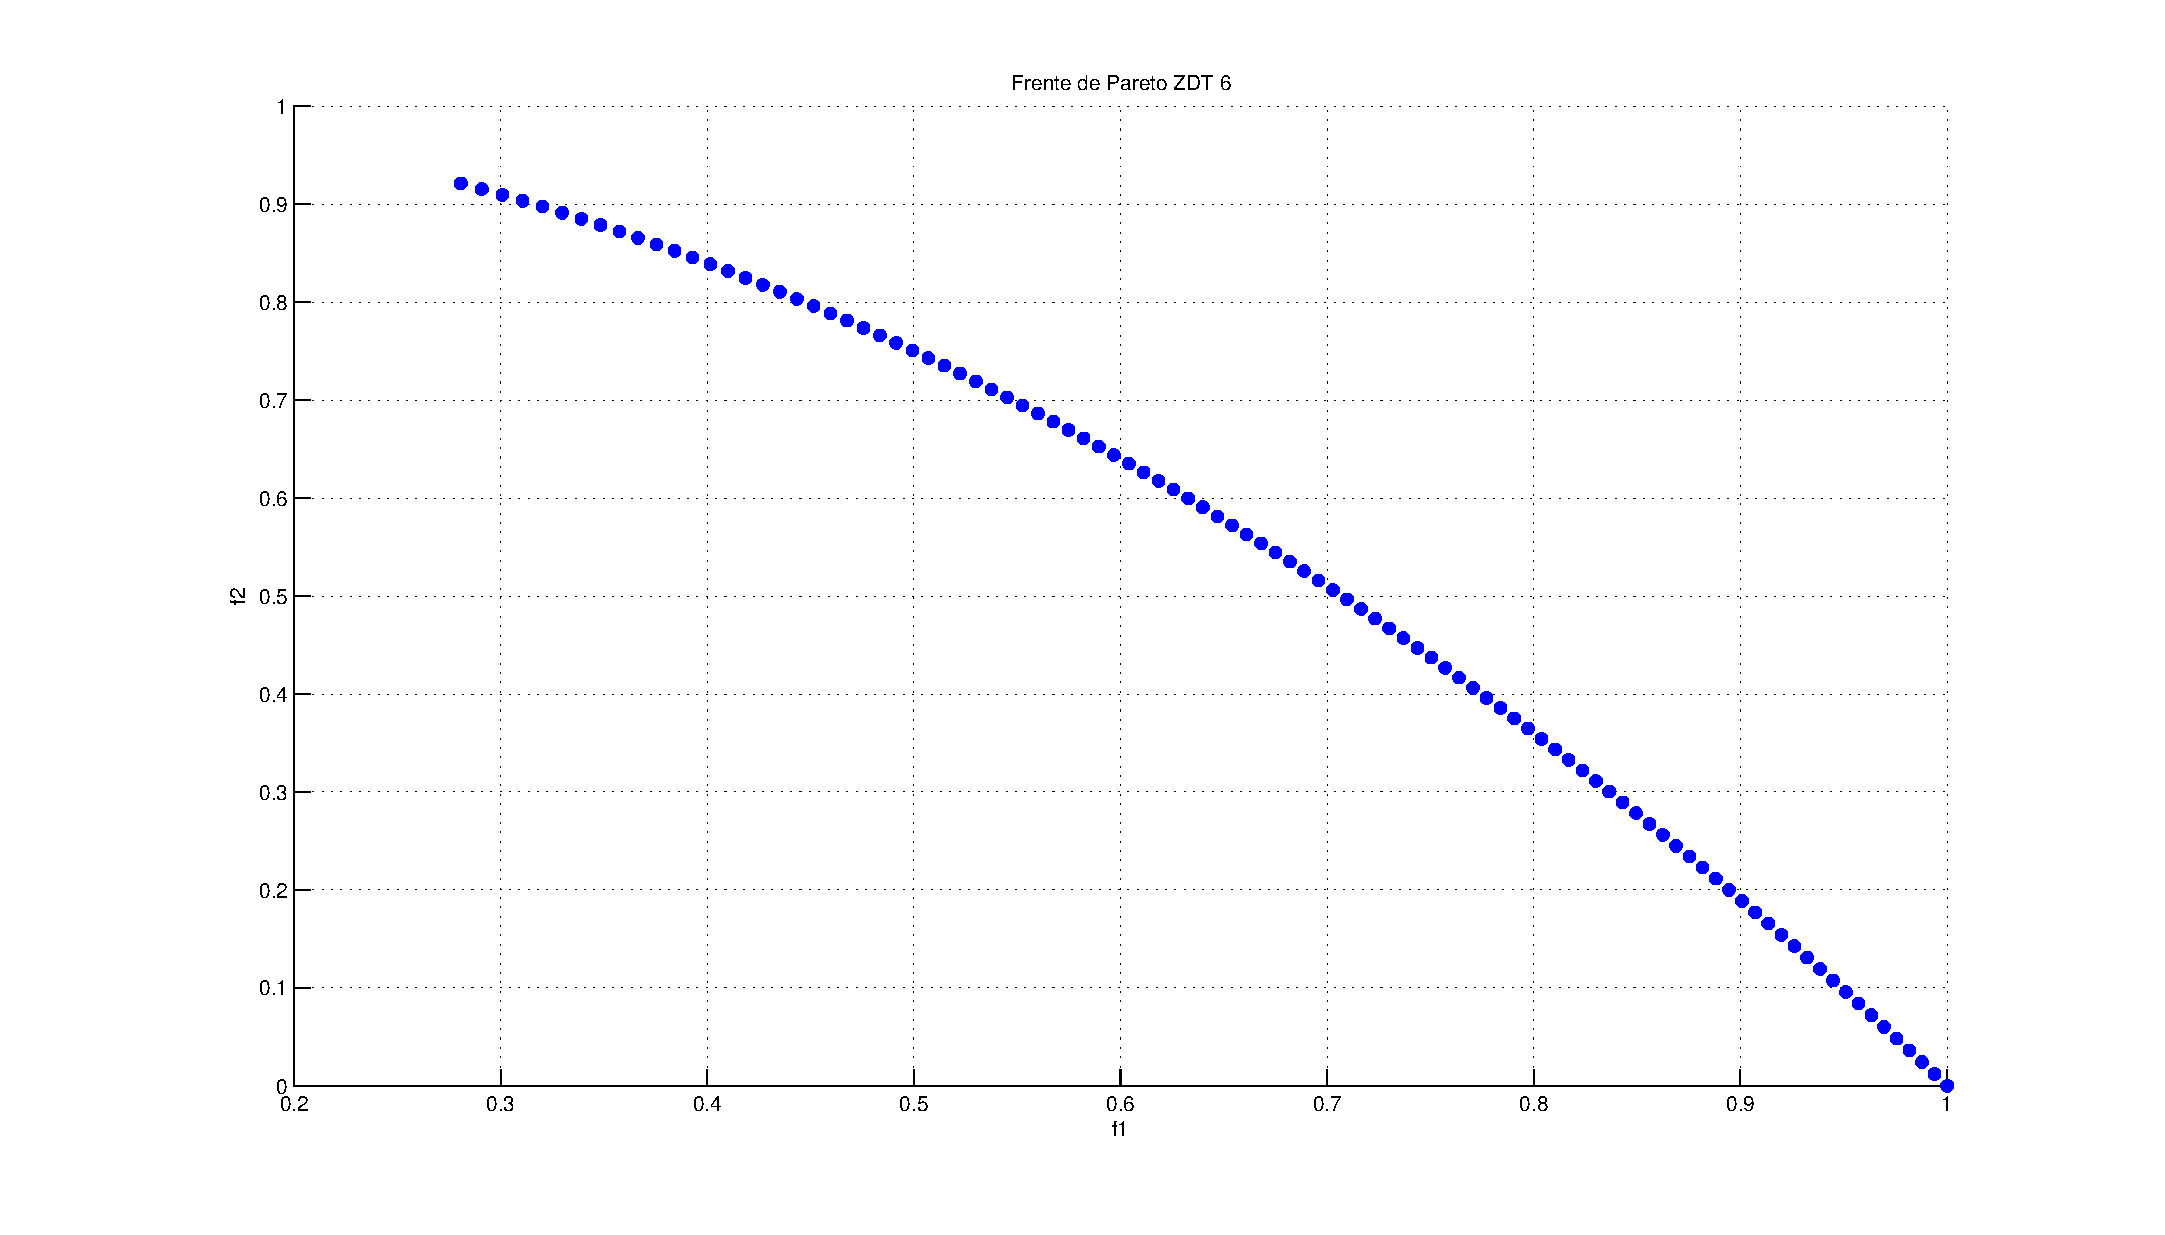
\includegraphics[scale=0.4]{ApendiceA/paretoZDT6.eps}
    \caption{Frente de Pareto verdadero de ZDT6}
    \label{fig:zdt6}
 
\end{figure}

\section{Evaluaci\'on del conjunto de problemas ZDT}

\begin{table}
  \begin{center}
    \begin{tabular}{|l||c|}
	\hline
	Problema  & Punto de referencia \\ 
	\hline
	\hline
	ZDT1 & $(1.1,1.1)$ \\ 
	\hline
	ZDT2 &  $(1.1,1.1)$\\
	\hline
	ZDT3 &  $(1.1,1.1)$\\
	\hline
	ZDT4 &  $(0.9,1.1)$\\
	\hline
	ZDT6 &  $(1.1,1.1)$\\
	\hline
  \end{tabular}
  \caption{Puntos de referencia utilizados para el conjunto de problemas ZDT}
  \label{tab:ref}
\end{center}
\end{table}

 \begin{table}
 \begin{center}
  \begin{tabular}{|l||cc|cc|} \hline
    & \multicolumn{4}{|c|}{\textbf{Espaciado}} \\     
	\textbf{Algoritmo} & \textbf{Menor} & \textbf{Mayor} & \textbf{Promedio} & \textbf{Desviaci\'on} \\  \hline \hline
	\textbf{MOPSOhv} &0.003157 & 0.004218 & 0.003524 & 0.000305  \\ 
	\textbf{MOPSOcd} &0.006072 & 0.007475 & 0.006962 & 0.000362  \\ 
	\textbf{NSGA-II} &0.005950 & 0.007813 & 0.007020 & 0.000447   \\  
	\textbf{SMS-EMOA}&0.001840 & 0.002976 & 0.002320 & 0.000270  \\  
	\hline\hline
    & \multicolumn{4}{|c|}{\textbf{DGI}} \\  \hline \hline
	\textbf{MOPSOhv} &0.017011 & 0.017021 & 0.017014 & 0.000003  \\ 
	\textbf{MOPSOcd} &0.017092 & 0.017240 & 0.017173 & 0.000036 \\ 
	\textbf{NSGA-II} &0.017008 & 0.017021 & 0.017011 & 0.000003 \\  
	\textbf{SMS-EMOA}&0.017008 & 0.017010 & 0.017009 & 0.000001   \\  
	\hline\hline
    & \multicolumn{4}{|c|}{\textbf{Hipervolumen}} \\ \hline\hline 
	\textbf{MOPSOhv} &0.871620 & 0.871991 & 0.871849 & 0.000095  \\ 
	\textbf{MOPSOcd} &0.861718 & 0.868142 & 0.864645 & 0.001562 \\ 
	\textbf{NSGA-II} &0.870107 & 0.871006 & 0.870461 & 0.000206 \\  
	\textbf{SMS-EMOA}&0.872115 & 0.872134 & 0.872129 & 0.000006 \\  
	\hline\hline
   & \multicolumn{4}{|c|}{\textbf{Cobertura}} \\ \hline\hline 
	\textbf{Algoritmo} & \textbf{MOPSOhv} & \textbf{MOPSOcd} & \textbf{NSGA-II} & \textbf{SMS-EMOA} \\  \hline \hline
	\textbf{MOPSOhv} & ---      & 0.722500  & 0.074500 & 0.000001  \\ 
	\textbf{MOPSOcd} & 0.000001 & ---       & 0.005500 & 0.000001 \\ 
	\textbf{NSGA-II} & 0.022500 & 0.618000  & ---      & 0.013500 \\  
	\textbf{SMS-EMOA}& 0.028500 & 0.762500  & 0.053500 & --- \\  
	\hline
	\end{tabular}
    \caption{Resultados correspondientes al problema ZDT1.}
  \label{tab:zdt1}
\end{center}
\end{table}
\newpage
    \begin{figure}
      \centering
	%\begin{rotate}{0}
	  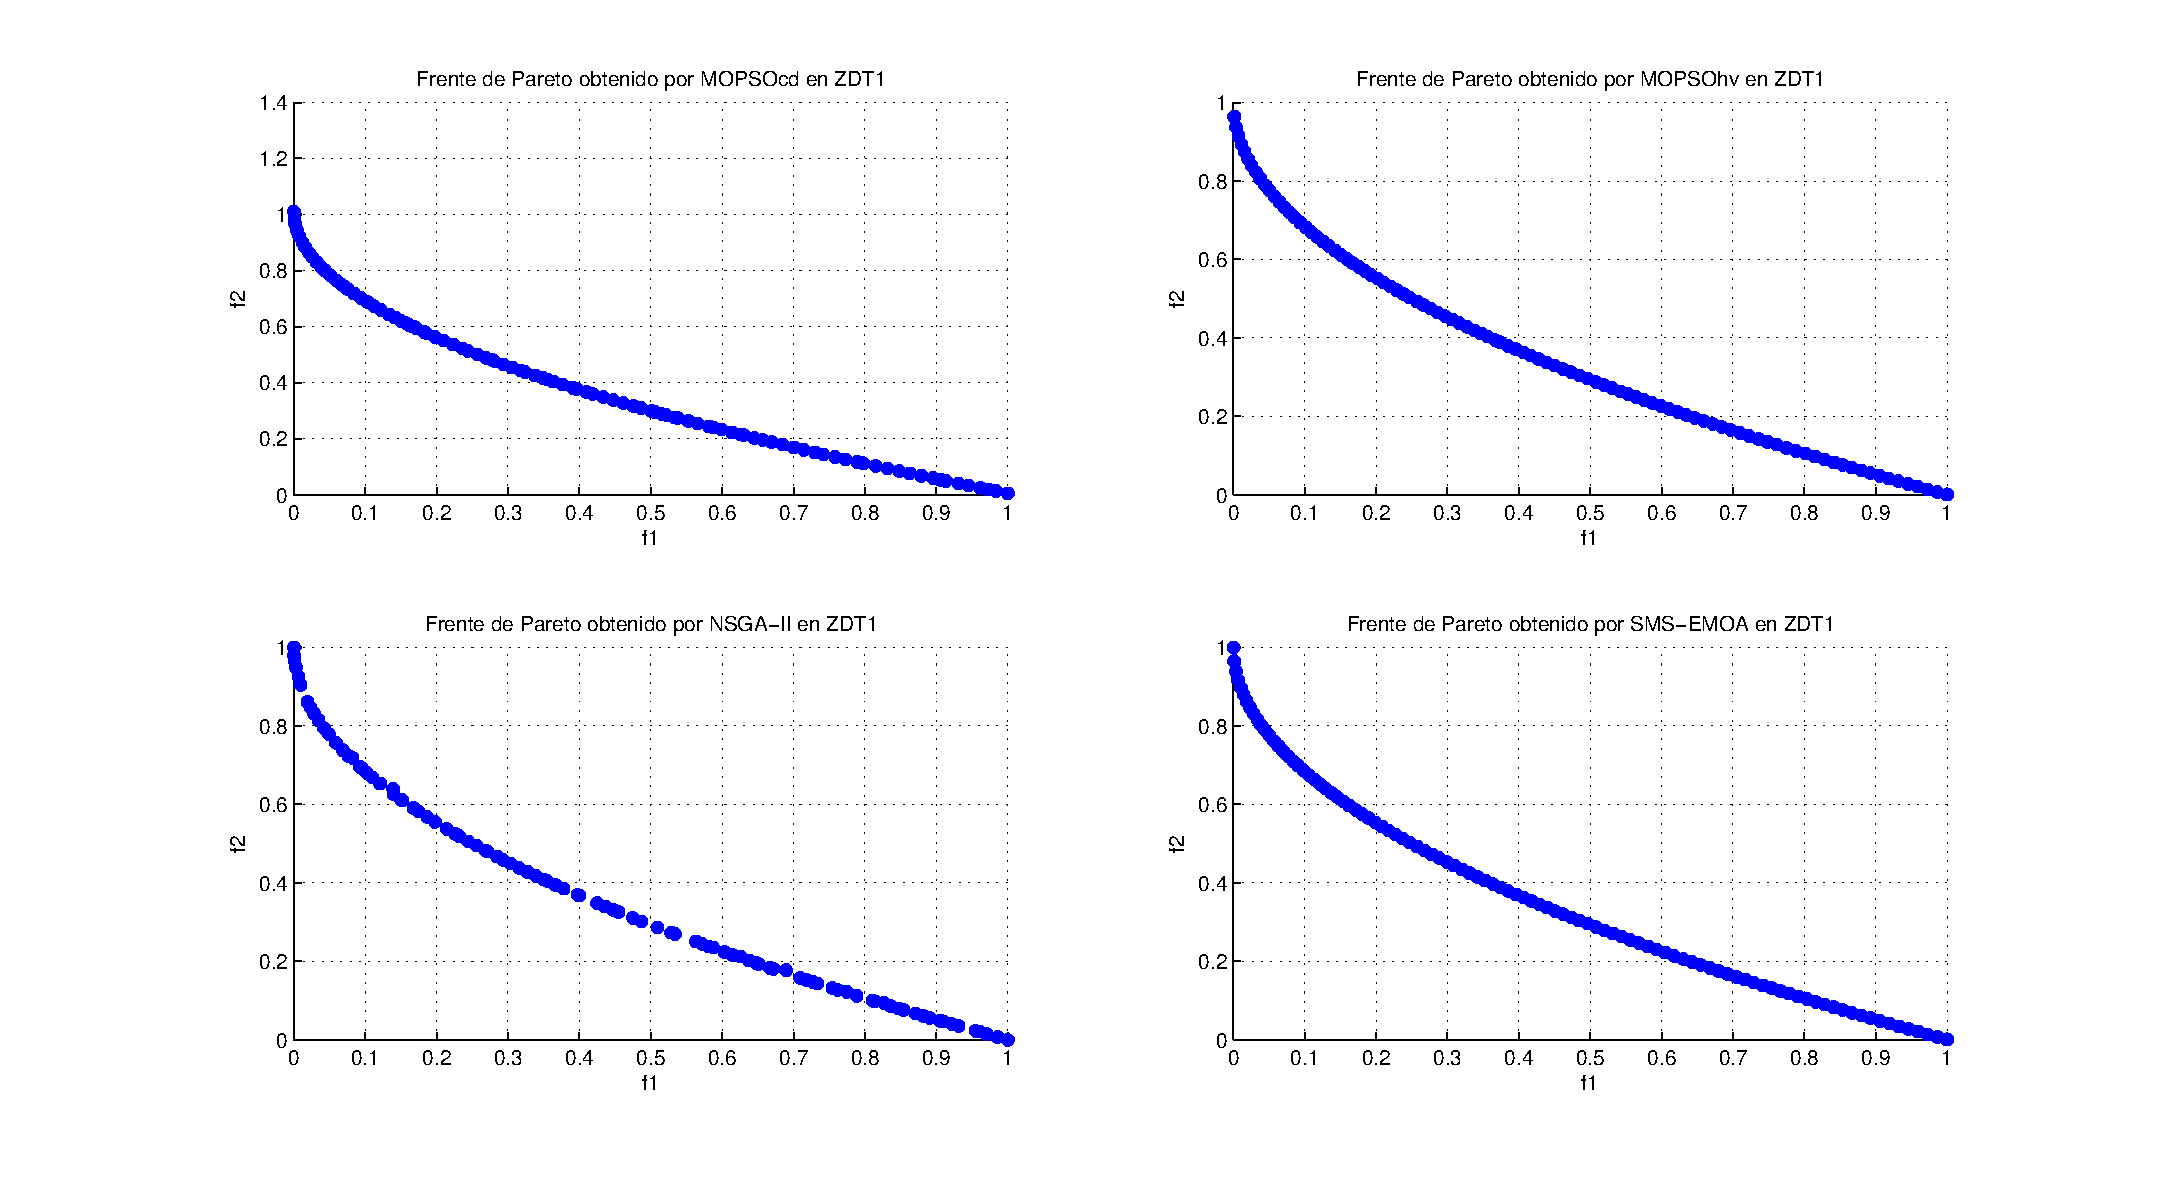
\includegraphics[scale=0.45]{Cap4/rzdt1r.eps}      
%	  \end{rotate}
	\caption{Resultados gr\'aficos correspondientes al problema ZDT1.}
      \label{fig:rZDT1}
      \end{figure}
\clearpage
\newpage
 \begin{table}
 \begin{center}
  \begin{tabular}{|l|cc|cc|} \hline
    & \multicolumn{4}{|c|}{\textbf{Espaciado}} \\ 
	\textbf{Algoritmo} & \textbf{Menor} & \textbf{Mayor} & \textbf{Promedio} & \textbf{Desviaci\'on} \\  \hline\hline
	\textbf{MOPSOhv} &0.004345 & 0.005129 & 0.004679 & 0.000217  \\ 
	\textbf{MOPSOcd} &0.006054 & 0.007826 & 0.007014 & 0.000517 \\ 
	\textbf{NSGA-II} &0.006027 & 0.008074 & 0.006956 & 0.000610  \\  
	\textbf{SMS-EMOA}&0.002167 & 0.004664 & 0.004063 & 0.000543  \\  
	\hline\hline
    & \multicolumn{4}{|c|}{\textbf{DGI}} \\ \hline \hline	
	\textbf{MOPSOhv} &0.027389 & 0.027394 & 0.027391 & 0.000001  \\ 
	\textbf{MOPSOcd} &0.027462 & 0.027521 & 0.027497 & 0.000015  \\ 
	\textbf{NSGA-II} &0.027386 & 0.027389 & 0.027387 & 0.000001  \\  
	\textbf{SMS-EMOA}&0.027386 & 0.027387 & 0.027386 & 0.000000  \\  
	\hline\hline
    & \multicolumn{4}{|c|}{\textbf{Hipervolumen}} \\ 	\hline \hline
	\textbf{MOPSOhv} &0.538426 & 0.538666 & 0.538568 & 0.000058 \\ 
	\textbf{MOPSOcd} &0.530732 & 0.534137 & 0.532098 & 0.000882   \\ 
	\textbf{NSGA-II} &0.537163 & 0.537699 & 0.537424 & 0.000148  \\  
	\textbf{SMS-EMOA}&0.538808 & 0.538879 & 0.538872 & 0.000015  \\  
	\hline\hline
    & \multicolumn{4}{|c|}{\textbf{Cobertura}} \\ \hline\hline 
	\textbf{Algoritmo} & \textbf{MOPSOhv} & \textbf{MOPSOcd} & \textbf{NSGA-II} & \textbf{SMS-EMOA} \\  \hline \hline
	\textbf{MOPSOhv} &---       & 0.637500 & 0.044000  & 0.000500 \\ 
	\textbf{MOPSOcd} & 0.000001 & ---      & 0.003500  & 0.000500 \\ 
	\textbf{NSGA-II} & 0.036500 & 0.589500 & ---      & 0.017500  \\  
	\textbf{SMS-EMOA}& 0.026500 & 0.665000 & 0.034000 & --- \\  
	\hline
	\end{tabular}
  \caption{Resultados correspondientes al problema ZDT2.}
  \label{tab:zdt2}
\end{center}
\end{table}
\clearpage
\newpage
\begin{figure}
      \begin{center}
	  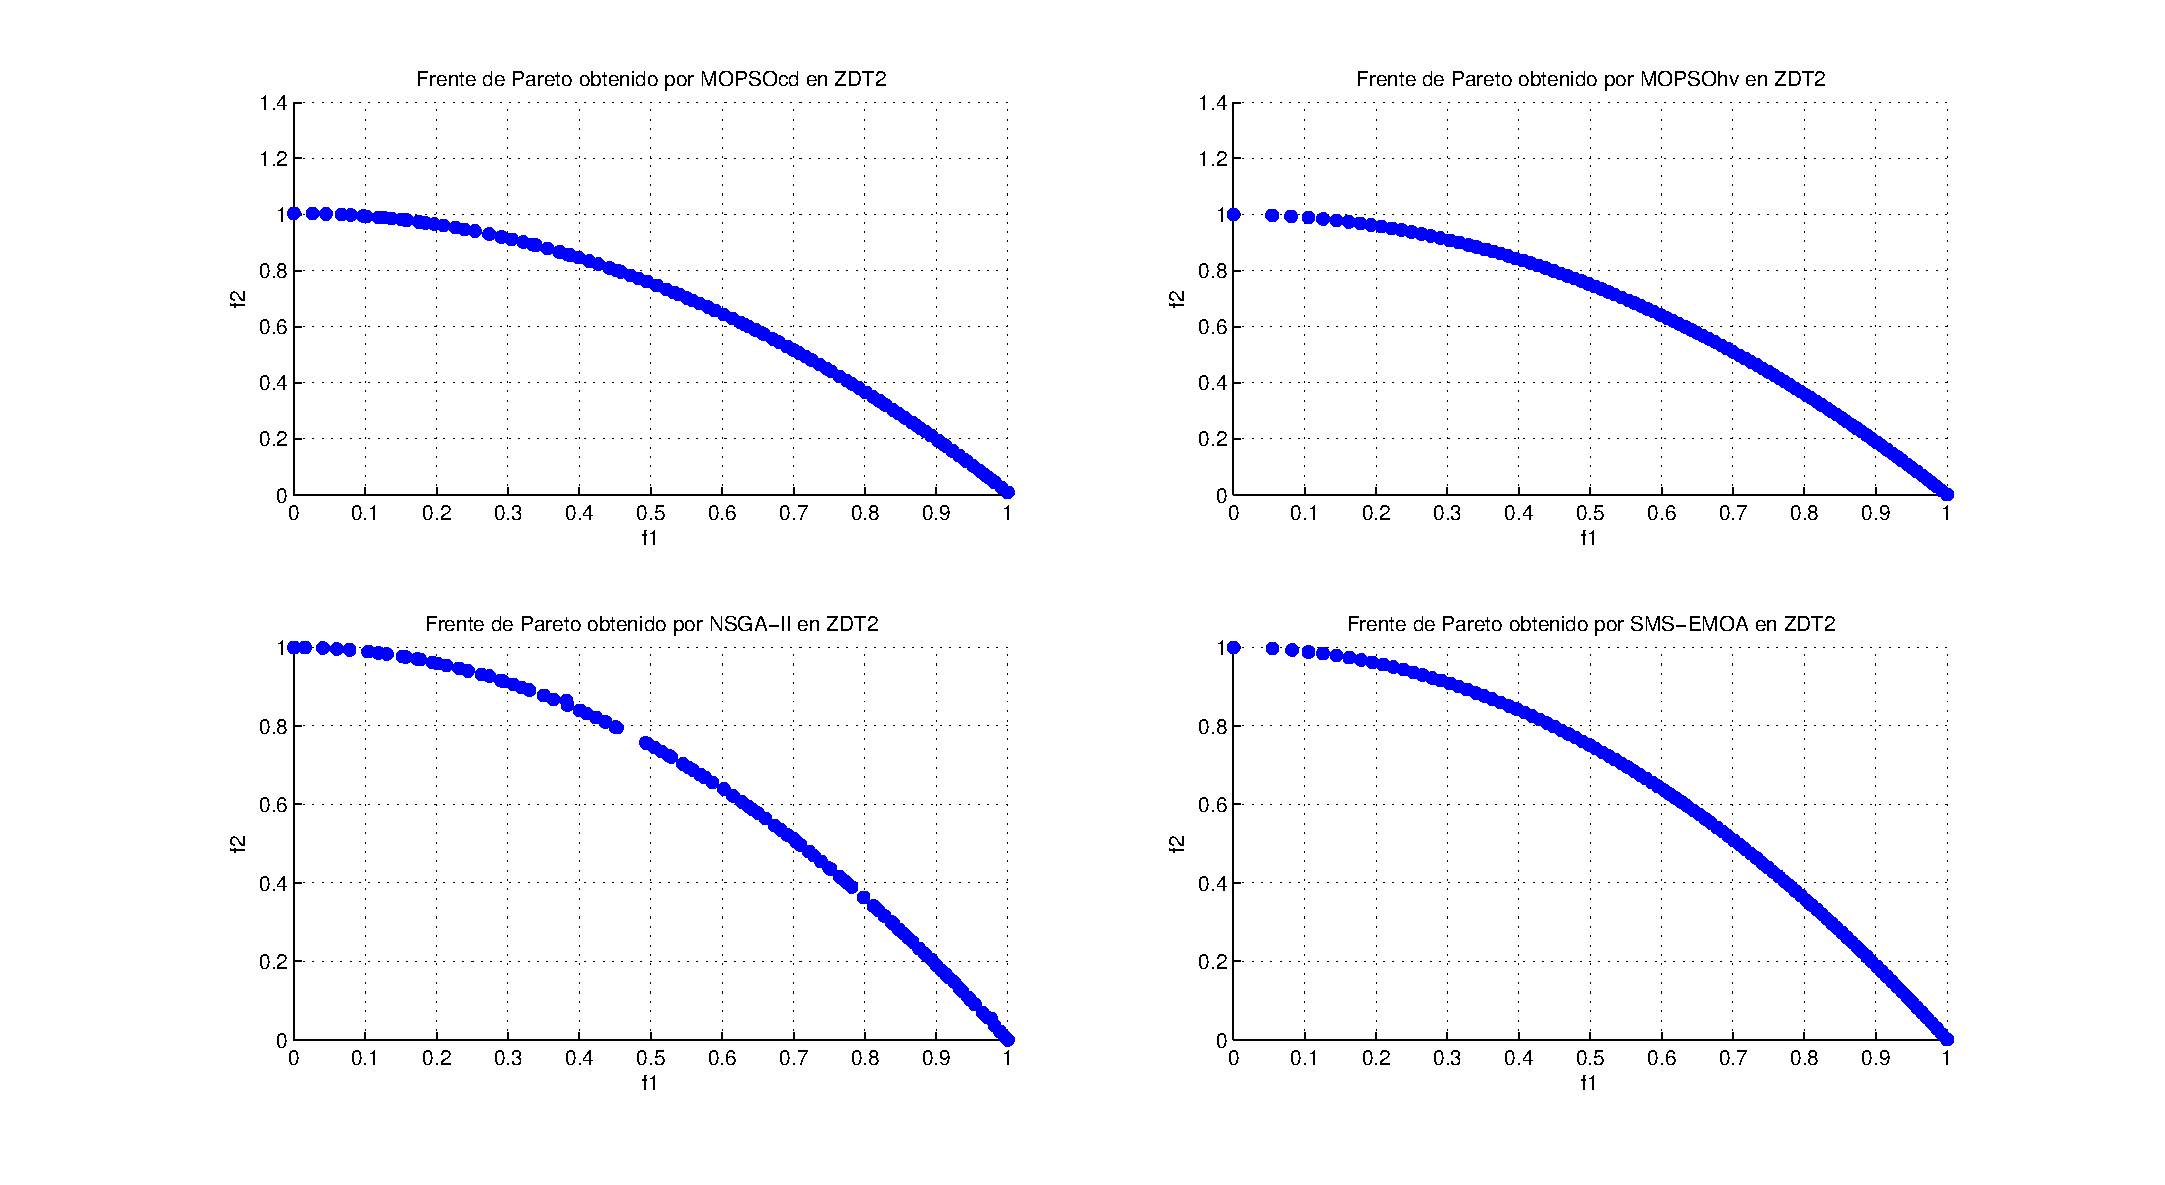
\includegraphics[scale=0.45]{Cap4/rzdt2r.eps}
      \end{center}
	\caption{Resultados gr\'aficos correspondientes al problema ZDT2.}
      \label{fig:rZDT2}
      \end{figure}
\clearpage
\newpage
 \begin{table}
 \begin{center}
  \begin{tabular}{|l|cc|cc|} \hline
    & \multicolumn{4}{|c|}{\textbf{Espaciado}} \\ 
	\textbf{Algoritmo} & \textbf{Menor} & \textbf{Mayor} & \textbf{Promedio} & \textbf{Desviaci\'on} \\  \hline\hline
	\textbf{MOPSOhv} &0.005672 & 0.006958 & 0.006248 & 0.000328  \\ 
	\textbf{MOPSOcd} &0.007001 & 0.008605 & 0.007656 & 0.000425 \\ 
	\textbf{NSGA-II} &0.006809 & 0.009101 & 0.007875 & 0.000565 \\  
	\textbf{SMS-EMOA}&0.001994 & 0.002563 & 0.002209 & 0.000165 \\  
	\hline\hline
    & \multicolumn{4}{|c|}{\textbf{DGI}} \\ 	\hline \hline
	\textbf{MOPSOhv} &0.011174 & 0.011219 & 0.011198 & 0.000012 \\ 
	\textbf{MOPSOcd} &0.011389 & 0.011604 & 0.011492 & 0.000064 \\ 
	\textbf{NSGA-II} &0.011140 & 0.011184 & 0.011166 & 0.000016 \\  
	\textbf{SMS-EMOA}&0.019892 & 0.019894 & 0.019892 & 0.000000 \\  
	\hline\hline
    & \multicolumn{4}{|c|}{\textbf{Hipervolumen}} \\ \hline \hline
	\textbf{MOPSOhv} &0.952055 & 0.953776 & 0.952907 & 0.000452  \\ 
	\textbf{MOPSOcd} &0.936835 & 0.946304 & 0.941991 & 0.002510 \\ 
	\textbf{NSGA-II} &0.953544 & 0.954219 & 0.953912 & 0.000145  \\  
	\textbf{SMS-EMOA}&0.522460 & 0.522466 & 0.522464 & 0.000001  \\  
	\hline
    & \multicolumn{4}{|c|}{\textbf{Cobertura}} \\ \hline\hline 
	\textbf{Algoritmo} & \textbf{MOPSOhv} & \textbf{MOPSOcd} & \textbf{NSGA-II} & \textbf{SMS-EMOA} \\  \hline \hline
	\textbf{MOPSOhv} &---       & 0.637500 & 0.044000 & 0.000500 \\ 
	\textbf{MOPSOcd} & 0.000001 & ---      & 0.003500 & 0.000500 \\ 
	\textbf{NSGA-II} & 0.036500 & 0.589500 & ---      & 0.017500 \\  
	\textbf{SMS-EMOA}& 0.026500 & 0.665000 & 0.034000 & --- \\  
	\hline\hline
	\end{tabular}
\caption{Resultados correspondientes al problema ZDT3.}
  \label{tab:zdt3}
\end{center}
\end{table}
\clearpage
\newpage
\begin{figure}
      \begin{center}
	  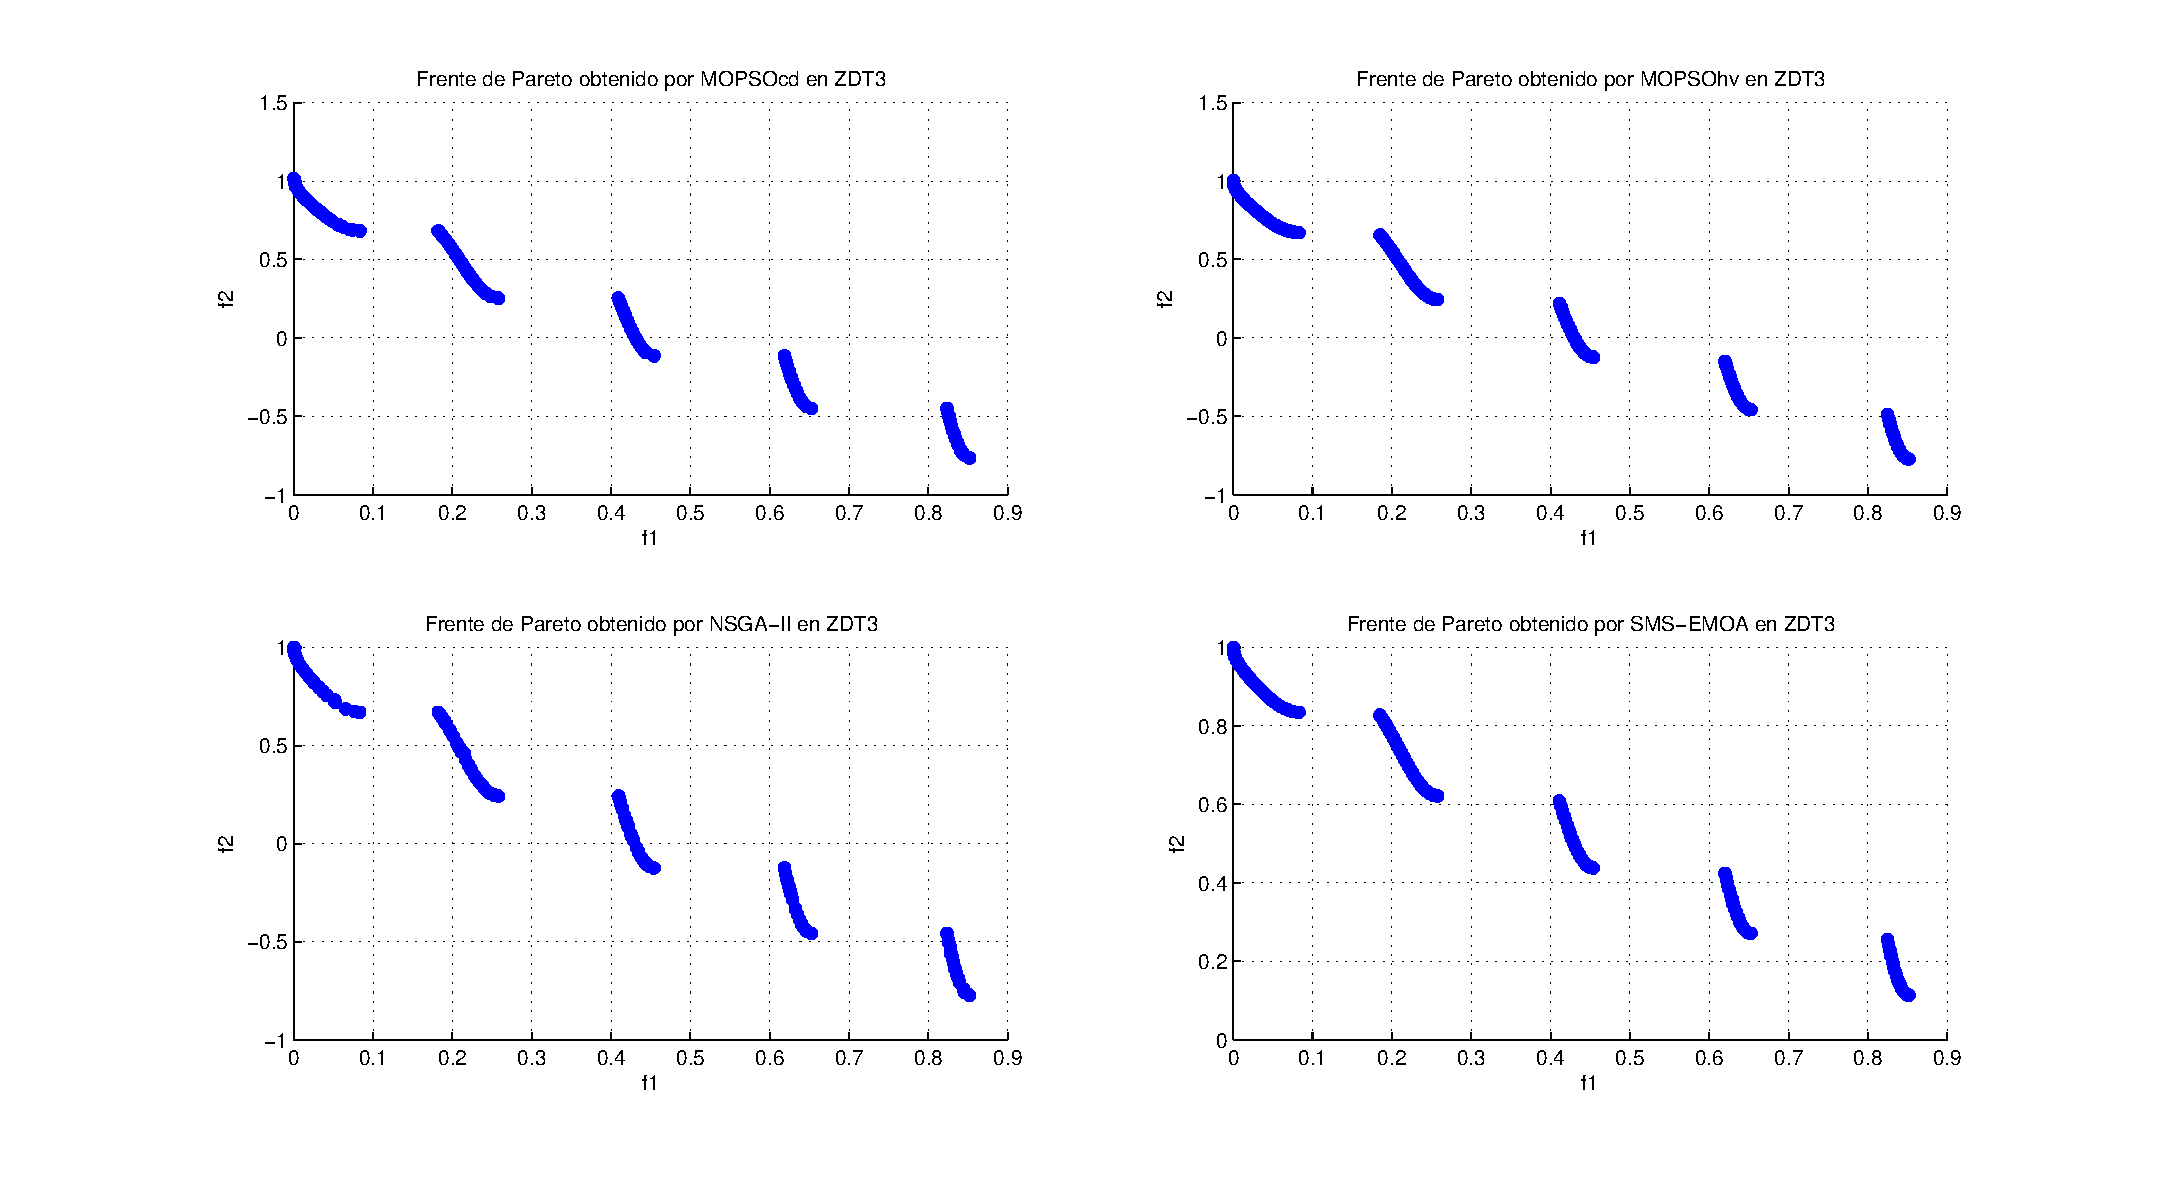
\includegraphics[scale=0.45]{Cap4/rzdt3r.eps}
      \end{center}
	\caption{Resultados gr\'aficos correspondientes al problema ZDT3.}
      \label{fig:rZDT3}
      \end{figure}
\clearpage
\newpage
 \begin{table}
 \begin{center}
  \begin{tabular}{|l|cc|cc|} \hline
    & \multicolumn{4}{|c|}{\textbf{Espaciado}} \\ 
	\textbf{Algoritmo} & \textbf{Menor} & \textbf{Mayor} & \textbf{Promedio} & \textbf{Desviaci\'on} \\  \hline\hline
	\textbf{MOPSOhv} &0.004345 & 0.005129 & 0.004679 & 0.000217 \\ 
	\textbf{MOPSOcd} &0.006054 & 0.007826 & 0.007014 & 0.000517  \\ 
	\textbf{NSGA-II} &0.007089 & 0.009201 & 0.008052 & 0.000616  \\  
	\textbf{SMS-EMOA}&0.002105 & 0.002981 & 0.002492 & 0.000240\\  
	\hline\hline
    & \multicolumn{4}{|c|}{\textbf{DGI}} \\ 	\hline \hline
	\textbf{MOPSOhv} &0.027389 & 0.027394 & 0.027391 & 0.000001   \\ 
	\textbf{MOPSOcd} &0.027462 & 0.027521 & 0.027497 & 0.000015  \\ 
	\textbf{NSGA-II} &0.017008 & 0.017016 & 0.017011 & 0.000002   \\  
	\textbf{SMS-EMOA}&0.017008 & 0.017030 & 0.017011 & 0.000004  \\  
	\hline\hline
    & \multicolumn{4}{|c|}{\textbf{Hipervolumen}} \\ 	\hline \hline
	\textbf{MOPSOhv} &0.328865 & 0.329046 & 0.328971 & 0.000052  \\ 
	\textbf{MOPSOcd} &0.323038 & 0.325624 & 0.324090 & 0.000668  \\ 
	\textbf{NSGA-II} &0.653158 & 0.654108 & 0.653614 & 0.000237  \\  
	\textbf{SMS-EMOA}&0.654266 & 0.655054 & 0.654940 & 0.000165  \\  
	\hline
    & \multicolumn{4}{|c|}{\textbf{Cobertura}} \\ \hline\hline 
	\textbf{Algoritmo} & \textbf{MOPSOhv} & \textbf{MOPSOcd} & \textbf{NSGA-II} & \textbf{SMS-EMOA} \\  \hline \hline
	\textbf{MOPSOhv} & ---      & 1.000000 & 0.022500 & 0.033000 \\ 
	\textbf{MOPSOcd} & 0.000500 & ---      & 0.000001 & 0.000001   \\ 
	\textbf{NSGA-II} & 0.004000 & 1.000000 & ---      & 0.024500 \\  
	\textbf{SMS-EMOA}& 0.000001 & 0.991000 & 0.001000 & --- \\  
	\hline\hline
	\end{tabular}
\caption{Resultados del problema ZDT4.}
  \label{tab:zdt4}
\end{center}
\end{table}
 \clearpage
 \newpage
 \begin{figure}
      \begin{center}
	  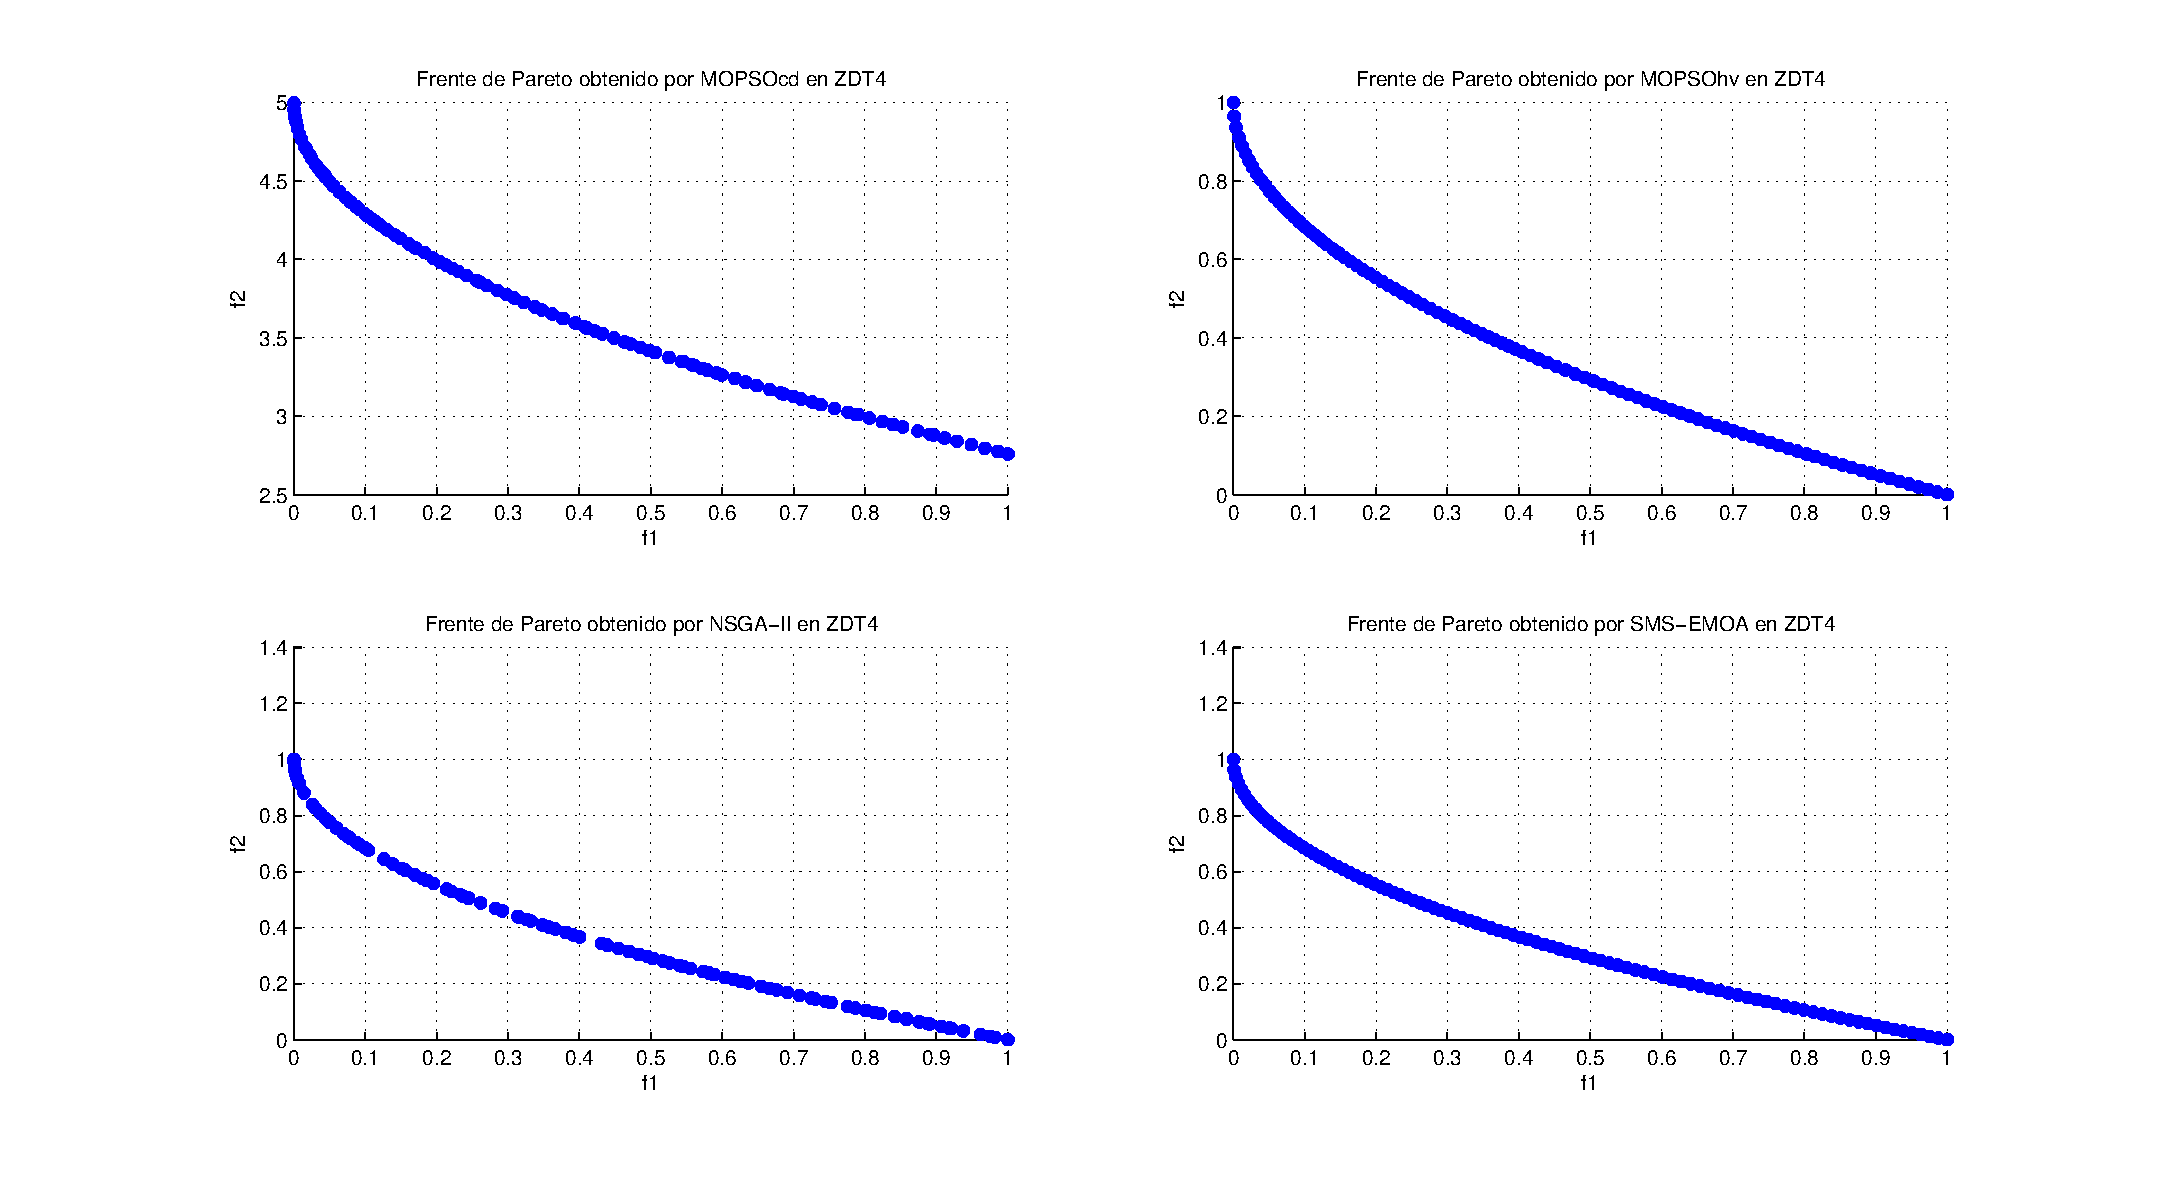
\includegraphics[scale=0.45]{Cap4/rzdt4r.eps}
      \end{center}
	\caption{Resultados gr\'aficos correspondientes al problema ZDT4.}
      \label{fig:rZDT4}
      \end{figure}
 \clearpage
 \newpage
 \begin{table}
 \begin{center}
  \begin{tabular}{|l|cc|cc|} \hline
    & \multicolumn{4}{|c|}{\textbf{Espaciado}} \\ 
	\textbf{Algoritmo} & \textbf{Menor} & \textbf{Mayor} & \textbf{Promedio} & \textbf{Desviaci\'on} \\  \hline\hline
	\textbf{MOPSOhv} &0.001587 & 0.002728 & 0.001975 & 0.000324  \\ 
	\textbf{MOPSOcd} &0.042774 & 0.294482 & 0.115691 & 0.05316 \\ 
	\textbf{NSGA-II} &0.005925 & 0.007914 & 0.007055 & 0.000437  \\  
	\textbf{SMS-EMOA}&0.000256 & 0.001011 & 0.000603 & 0.000181 \\  
	\hline\hline
    & \multicolumn{4}{|c|}{\textbf{DGI}} \\ 	\hline \hline
	\textbf{MOPSOhv} &0.027380 & 0.027549 & 0.027434 & 0.000046  \\ 
	\textbf{MOPSOcd} &0.000281 & 0.000281 & 0.000281 & 0.000000  \\ 
	\textbf{NSGA-II} &0.017011 & 0.027398 & 0.026356 & 0.003115  \\  
	\textbf{SMS-EMOA}&0.027390 & 0.027397 & 0.027395 & 0.000002  \\  
	\hline\hline
    & \multicolumn{4}{|c|}{\textbf{Hipervolumen}} \\ \hline \hline
	\textbf{MOPSOhv} &0.496939 & 0.54493 & 0.512122 & 0.002083  \\ 
	\textbf{MOPSOcd} &0.156527 & 0.479775 & 0.383107 & 0.076527 \\ 
	\textbf{NSGA-II} &0.480422 & 0.870700 & 0.519667 & 0.117011 \\  
	\textbf{SMS-EMOA}&0.503836 & 0.504173 & 0.503956 & 0.000093 \\  
	\hline\hline
    & \multicolumn{4}{|c|}{\textbf{Cobertura}} \\ \hline\hline 
	\textbf{Algoritmo} & \textbf{MOPSOhv} & \textbf{MOPSOcd} & \textbf{NSGA-II} & \textbf{SMS-EMOA} \\  \hline \hline
	\textbf{MOPSOhv} &---       & 0.127778 & 0.000001  & 0.000001 \\ 
	\textbf{MOPSOcd} & 0.059000 & ---      & 0.025500  & 0.019000  \\ 
	\textbf{NSGA-II} & 0.037500 & 0.645500 & ---       & 0.011000 \\  
	\textbf{SMS-EMOA}& 0.138889 & 0.850000 & 0.009000  & --- \\  
	\hline
	\end{tabular}
\caption{Resultados correspondientes al problema ZDT6.}
  \label{tab:zdt6}
\end{center}
\end{table}
\clearpage
\newpage
%\begin{landscape}

  \begin{figure}
      \begin{center}
	  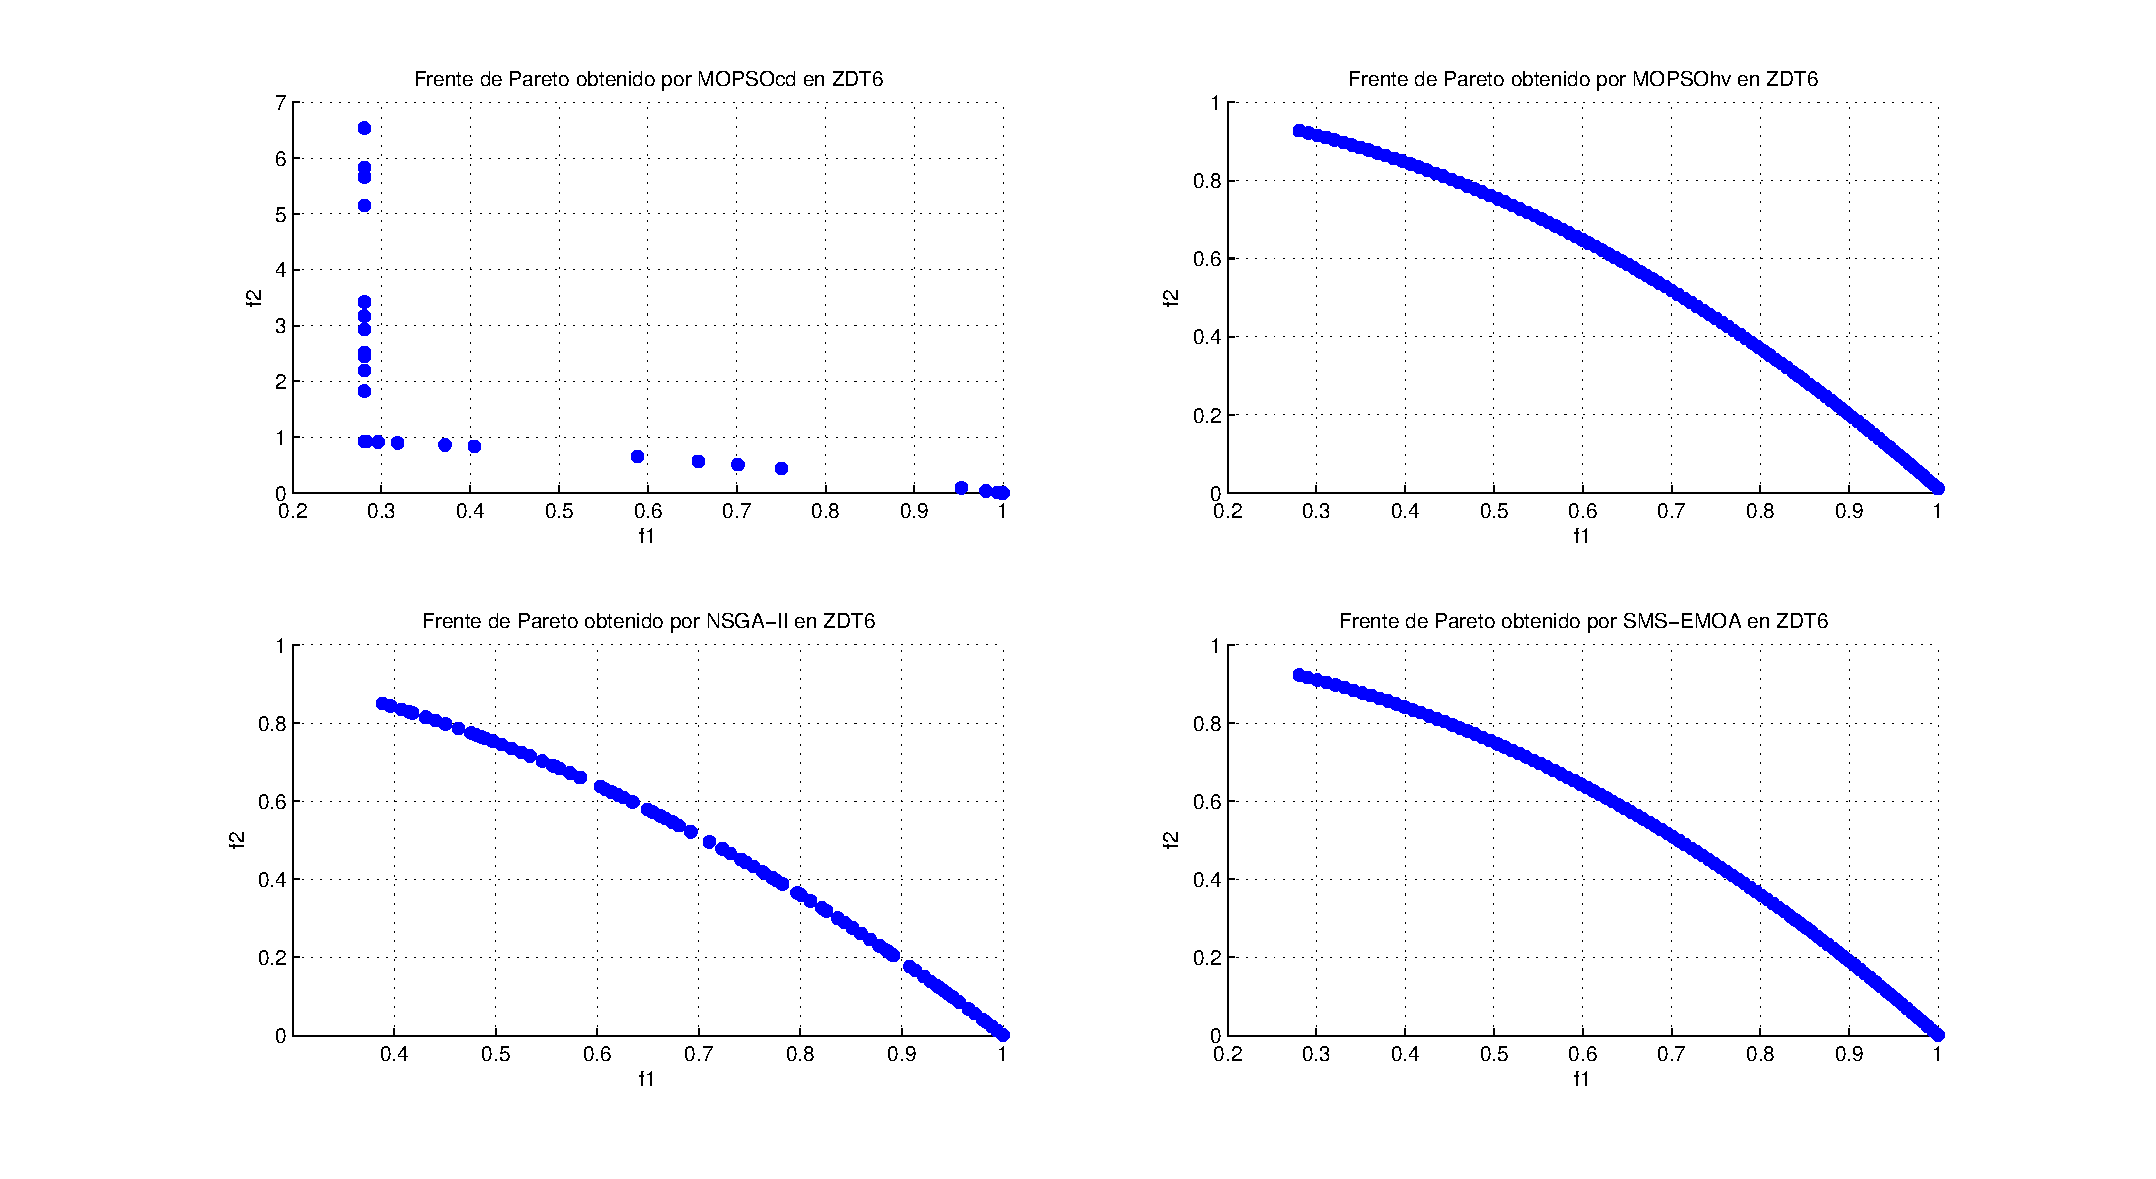
\includegraphics[scale=0.45]{Cap4/rzdt6r.eps}
      \end{center}
	\caption{Resultados gr\'aficos correspondientes al problema ZDT6.}
      \label{fig:rZDT6}
      \end{figure}
%\end{landscape}
\clearpage
   
  Los resultados obtenidos para los primeros tres problemas ZDT son similares, como se muestra en las tablas \ref{tab:zdt1}, 
  \ref{tab:zdt2} y \ref{tab:zdt6}. Los resultados gr\'aficos de estos tres primeros problemas ZDT se muestran en las 
  figuras \ref{fig:zdt1}, \ref{fig:zdt2} y \ref{fig:zdt3}. En ellos puede verse que, se tienen dos casos especiales (ZDT4 y ZDT5). El punto 
  de referencia utilizado en cada caso para el indicador del hipervolumen se muestra en la tabla \ref{tab:ref}.
  
  El problema ZDT4 tiene un frente de Pareto que es altamente multifrontal el cual consiste en $21^9$ frentes de Paretos locales.
  Nuestro propuesta obtiene, en general, mejores resultados que los obtenidos por el SMS-EMOA y marginalmente peores que los del NSGA-II.
  Los resultados obtenidos por el algoritmo MOPSOcd muestran que queda atrapado en un frente de Pareto local, por lo que,
  nuestra propuesta es mejor (los resultados se muestran en la tabla \ref{tab:zdt4} y en la figura \ref{fig:zdt4})
  
  El problema ZDT6 presenta un espacio de b\'usqueda no uniforme. Los resultados para este problema son ligeramente 
  mejores que los del SMS-EMOA y ligeramente peores que los del NSGA-II. Debido a la baja densidad de las soluciones obtenidas por 
  el algoritmo MOPSOcd, \'este no es capaz de alcanzar una buena aproximaci\'on al frente de Pareto real, por lo 1ue, nuestra propuesta es mejor
  (los resultados se muestran en la tabla \ref{tab:zdt6} y en la figura \ref{fig:zdt6})
  
\section{Conjunto de problemas DTLZ} 

Los problemas siguientes son parte de la serie de problemas DTLZ con tres funciones objetivo, tal y como se describen a continuaci\'on 
\cite{dtlz2002a}:

\begin{itemize}
\item La funci\'on de prueba \textbf{DTLZ1} tiene un frente de Pareto lineal, separable y multimodal:

\begin{align*}
f_1(x)&=\frac{1}{2}\cdot x_1\cdot x_2 \cdot \ldots \cdot x_{M-1} \cdot (1+g(x))\\
f_2(x)&=\frac{1}{2}\cdot x_1\cdot x_2 \cdot \ldots \cdot(1-x_{M-1})\cdot(1+g(x))\\
\vdots&\\
f_M(x)&=\frac{1}{2}\cdot(1-x_1)\cdot(1+g(x))\\
g(x)&=100\cdot[k+\sum_{i=M}^n(x_i-0.5)^2-cos(20\cdot\pi\cdot(x_i-0.5))]
\end{align*}

donde $n=M+k-1$ (se sugiere una $k=5$) y $x_i\in[0,1]$ con $i = 1, \ldots, n$ (figura \ref{fig:dtlz1}).


 \item La funci\'on de prueba \textbf{DTLZ2} tiene un frente de Pareto c\'oncavo:
\begin{align*}
f_1(x)&=\cos(x_1\frac{\pi}{2})\cdot\cos(x_2\frac{\pi}{2})\cdot\ldots\cdot\cos(x_{M-1}\frac{\pi}{2})\cdot(1+g(x))\\
f_2(x)&=\cos(x_1\frac{\pi}{2})\cdot\cos(x_2\frac{\pi}{2})\cdot\ldots\cdot\sin(x_{M-1}\frac{\pi}{2})\cdot(1+g(x))\\
f_3(x)&=\cos(x_1\frac{\pi}{2})\cdot\cos(x_2\frac{\pi}{2})\cdot\ldots\cdot\sin(x_{M-2}\frac{\pi}{2})\cdot(1+g(x))\\
\vdots&\\
f_{M-1}(x)&=\cos(x_1\frac{\pi}{2})\cdot\sin(x_2\frac{\pi}{2})(1+g(x))\\
f_{M}(x)&=\sin(x_1\frac{\pi}{2})\cdot(1+g(x))\\
g(x)&=\sum_i=(x_i-0.5)^2
\end{align*}

donde $n=M+k-1$ (se sugiere una $k=10$) y $x_i\in[0,1]$ con $i= 1, \ldots, n$. Este problema se puede utilizar para investigar la 
escalabilidad (figura \ref{fig:dtlz2}).

\item La funci\'on de prueba \textbf{DTLZ3} tiene un frente de Pareto c\'oncavo y multimodal:
\begin{align*}
f_1(x)&=\cos(x_1\frac{\pi}{2})\cdot\cos(x_2\frac{\pi}{2})\cdot\ldots\cdot \cos(x_{M-1}\frac{\pi}{2})\cdot(1+g(x))\\
f_2(x)&=\cos(x_1\frac{\pi}{2})\cdot\cos(x_2\frac{\pi}{2})\cdot\ldots\cdot \sin(x_{M-1}\frac{\pi}{2})\cdot(1+g(x))\\
f_3(x)&=\cos(x_1\frac{\pi}{2})\cdot\cos(x_2\frac{\pi}{2})\cdot\ldots\cdot \sin(x_{M-2}\frac{\pi}{2})\cdot(1+g(x))\\
\vdots&\\
f_{M-1}(x)&=\cos(x_1\frac{\pi}{2})\cdot\sin(x_2\frac{\pi}{2})\cdot(1+g(x))\\
f_{M}(x)&=\sin(x_1\frac{\pi}{2})\cdot (1+g(x))\\
g(x)&=100\cdot [k+\sum_{i=M}^n(x_i-0.5)^2-\cos(20\cdot\pi\cdot(x_i-0.5))]
\end{align*}

donde $n=M+k-1$ (se sugiere una $k=10$) y $x_i\in[0,1]$ con $i=1, \ldots, n$ (figura \ref{fig:dtlz3}).

\item La funci\'on de prueba \textbf{DTLZ4} tiene un frente de Pareto c\'oncavo, separable y multimodal:

\begin{align*}
f_1(x)&=\cos(x_1^\alpha\frac{\pi}{2})\cdot\cos(x_2^\alpha\frac{\pi}{2})\cdot\ldots\cdot \cos(x_{M-1}^\alpha\frac{\pi}{2})\cdot(1+g(x))\\
f_2(x)&=\cos(x_1^\alpha\frac{\pi}{2})\cdot\cos(x_2^\alpha\frac{\pi}{2})\cdot\ldots\cdot \sin(x_{M-1}^\alpha\frac{\pi}{2})\cdot(1+g(x))\\
f_3(x)&=\cos(x_1^\alpha\frac{\pi}{2})\cdot\cos(x_2^\alpha\frac{\pi}{2})\cdot\ldots\cdot \sin(x_{M-2}^\alpha\frac{\pi}{2})\cdot(1+g(x))\\
\vdots&\\
f_{M-1}(x)&=\cos(x_1^\alpha\frac{\pi}{2})\cdot\sin(x_2^\alpha\frac{\pi}{2})\cdot(1+g(x))\\
f_{M}(x)&=\sin(x_1^\alpha\frac{\pi}{2})\cdot(1+g(x))\\
g(x)&=\sum_i(x_i-0.5)^2
\end{align*}

donde $n=M+k-1$ (se sugiere una $k=10$ y $\alpha=100$) y $x_i\in[0,1]$ con $i=1,\ldots, n$. Este probema prueba la habilidad de mantener 
una buena distribuci\'on de las soluciones (figura \ref{fig:dtlz4}).

\item \textbf La funci\'on de prueba \textbf{DTLZ5} tiene un frente de Pareto curvo:

\begin{align*}
f_1(x)&=\cos(\theta_1\frac{\pi}{2})\cdot\cos(\theta_2\frac{\pi}{2})\cdot\ldots\cdot \cos(\theta_{M-1}\frac{\pi}{2})\cdot(1+g(x))\\
f_2(x)&=\cos(\theta_1\frac{\pi}{2})\cdot\cos(\theta_2\frac{\pi}{2})\cdot\ldots\cdot \sin(\theta_{M-1}\frac{\pi}{2})\cdot(1+g(x))\\
f_3(x)&=\cos(\theta_1\frac{\pi}{2})\cdot\cos(\theta_2\frac{\pi}{2})\cdot\ldots\cdot \sin(\theta_{M-2}\frac{\pi}{2})\cdot(1+g(x))\\
\vdots&\\
f_{M-1}(x)&=\cos(\theta_1\frac{\pi}{2})\cdot\sin(\theta_2\frac{\pi}{2})\cdot(1+g(x))\\
f_{M}(x)&=\sin(\theta_1\frac{\pi}{2})\cdot(1+g(x))\\
\theta_1&=\frac{\pi}{2}x_1\\
\theta_i&=\frac{\pi}{4\cdot(1+g(x))}(1+2\cdot g(x)\cdot x_i),  \text{para} \hspace{1mm} i=2,3\dots,(M-1)\\
g(x)&=\sum^n_i(x_i-0.5)^2
\end{align*}

donde $n=M+k-1$ (se sugiere una $k=10$) y $x_i\in[0,1]$ con $i = 1,\ldots,n$ (figura \ref{fig:dtlz5}).

\item La funci\'on de prueba \textbf{DTLZ6} tiene un frente de Pareto curvo:

\begin{align*}
f_1(x)&=\cos(\theta_1\frac{\pi}{2})\cdot\cos(\theta_2\frac{\pi}{2})\cdot\ldots\cdot \cos(\theta_{M-1}\frac{\pi}{2})\cdot(1+g(x))\\
f_2(x)&=\cos(\theta_1\frac{\pi}{2})\cdot\cos(\theta_2\frac{\pi}{2})\cdot\ldots\cdot \sin(\theta_{M-1}\frac{\pi}{2})\cdot(1+g(x))\\
f_3(x)&=\cos(\theta_1\frac{\pi}{2})\cdot\cos(\theta_2\frac{\pi}{2})\cdot\ldots\cdot \sin(\theta_{M-2}\frac{\pi}{2})\cdot(1+g(x))\\
\vdots&\\
f_{M-1}(x)&=\cos(\theta_1\frac{\pi}{2})\cdot\sin(\theta_2\frac{\pi}{2})\cdot(1+g(x))\\
f_{M}(x)&=\sin(\theta_1\frac{\pi}{2})\cdot(1+g(x))\\
\theta_1&=\frac{\pi}{2}x_1\\
\theta_i&=\frac{\pi}{4(1+g(x))}(1+2\cdot g(x)\cdot x_i),  \text{para}\hspace{1mm} i=2,3\dots,(M-1)\\
g(x)&=\sum^n_i=(x_i-0.5)^0.1
\end{align*}

donde $n=M+k-1$ (se sugiere una $k=10$) y $x_i\in[0,1]$ con $i=1,\ldots,n$ (figura \ref{fig:dtlz6}).

\item La funci\'on de prueba \textbf{DTLZ7} tiene un frente de Pareto discontinuo:

\begin{align*}
f_1(x)&=x_1 \\
f_2(x)&=x_2\\
\vdots&\\
f_{M-1}(x)&=x_{M-1}\\
f_{M}(x)&=(1+g(x_M))\cdot h(f_1,f_2,\dots,f_{M-1}g(x))\\
g(x)&=1+\frac{9}{k}\cdot\sum_{i=2}^nx_i\\
h(f_1,f_2,\dots,f_{M-1}g(x))&=M-\sum_{i=1}^{M-1}(\frac{f_i}{1+g(x)}(1+\sin{(3\cdot\pi\cdot f_i)}))
\end{align*}

donde $n=M+k-1$ (se sugiere una $k=20$) y $x_i\in[0,1]$ con $i=1,\ldots,n$. Este problema prueba la habilidad de mantener 
individuos en las diferentes regiones del frente de Pareto (figura \ref{fig:dtlz7}).

\end{itemize}


\begin{figure}
    \centering
    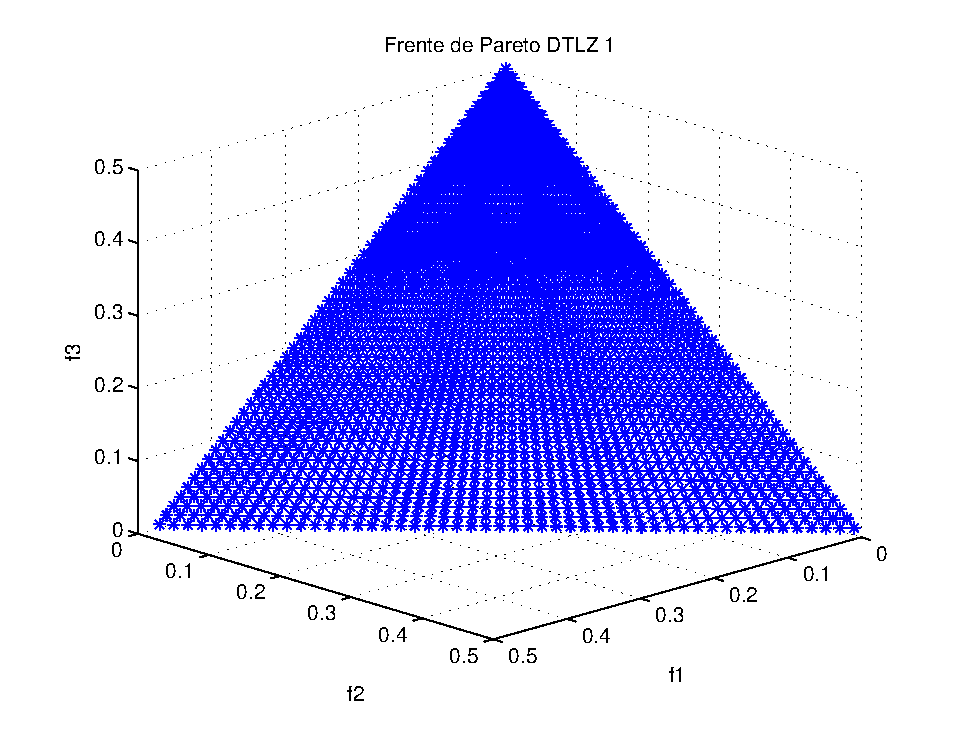
\includegraphics[scale=0.7]{ApendiceA/paretoDTLZ1.eps}
    \caption{Frente de Pareto verdadero de DTLZ1}
    \label{fig:dtlz1}
\end{figure}

\begin{figure}
    \centering
    \includegraphics[scale=0.7]{ApendiceA/paretoDTLZ2.eps}
    \caption{Frente de Pareto verdadero de DTLZ2}
    \label{fig:dtlz2}
\end{figure}
\begin{figure}
    \centering
    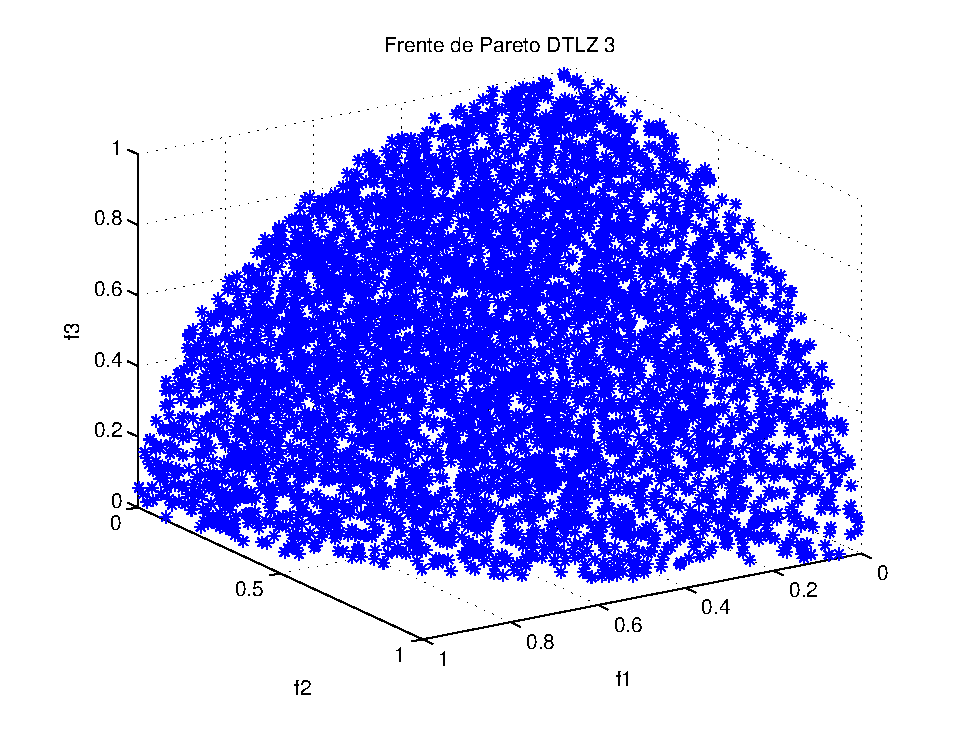
\includegraphics[scale=0.7]{ApendiceA/paretoDTLZ3.eps}
    \caption{Frente de Pareto verdadero de DTLZ3}
    \label{fig:dtlz3}
\end{figure}
\begin{figure}
    \centering
    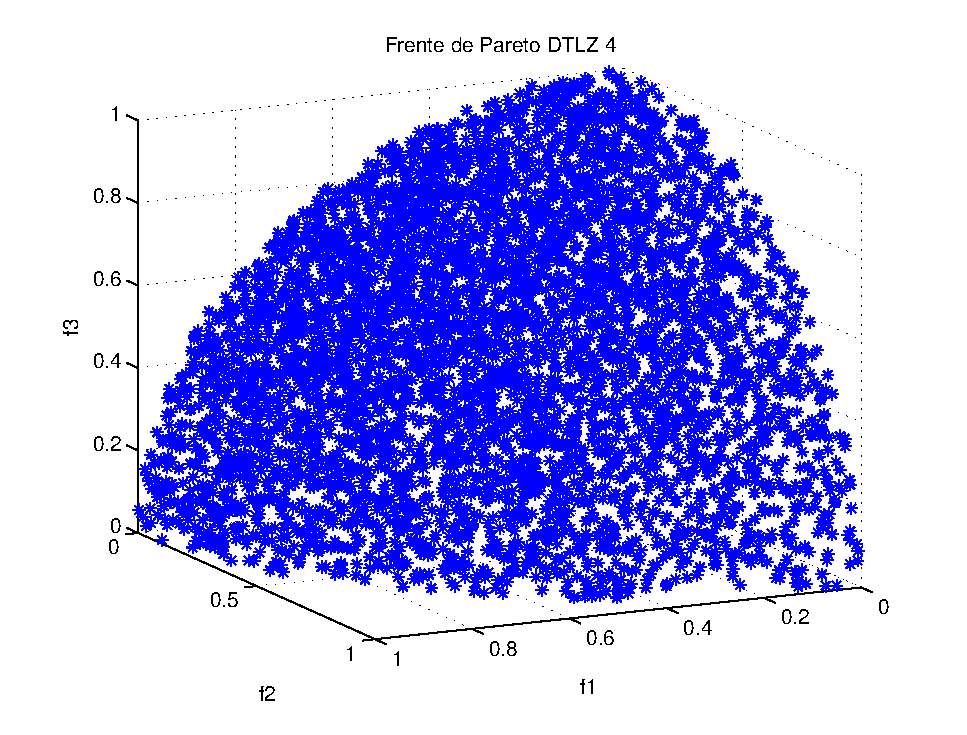
\includegraphics[scale=0.7]{ApendiceA/paretoDTLZ4.eps}
    \caption{Frente de Pareto verdadero de DTLZ4}
    \label{fig:dtlz4}
\end{figure}
\begin{figure}
    \centering
    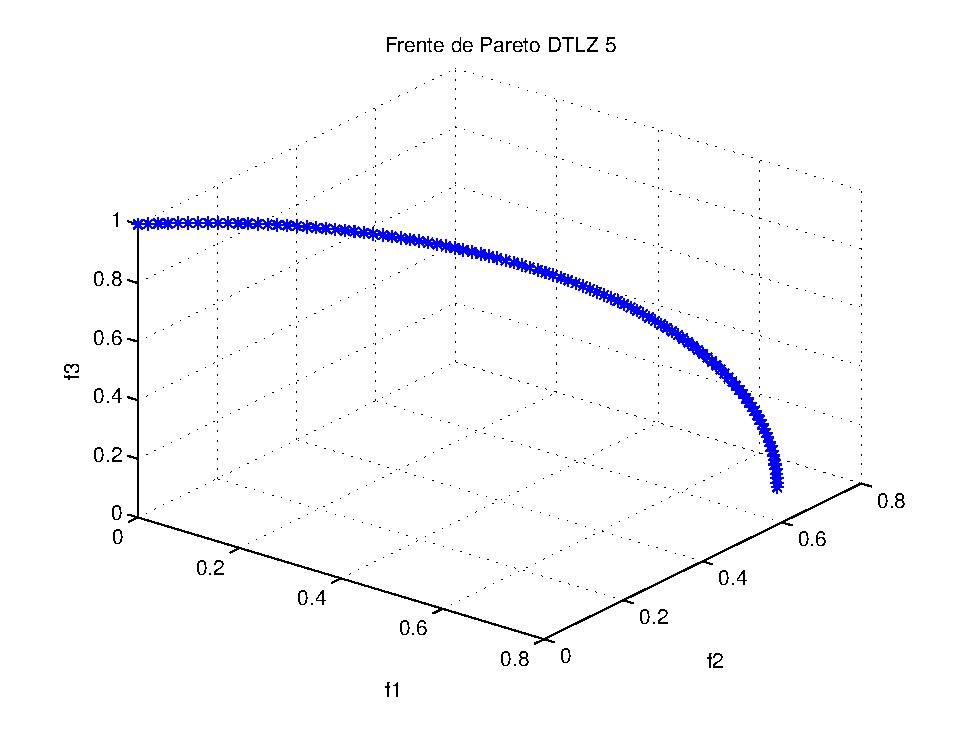
\includegraphics[scale=0.7]{ApendiceA/paretoDTLZ5.eps}
    \caption{Frente de Pareto verdadero de DTLZ5}
    \label{fig:dtlz5}
\end{figure}
\begin{figure}
  \centering
    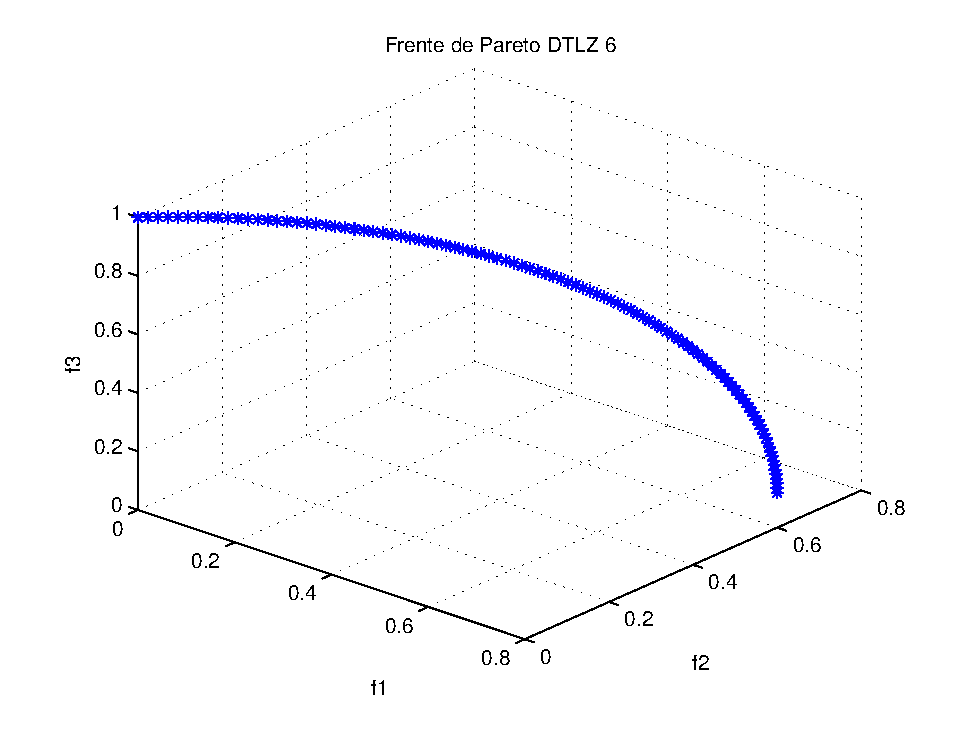
\includegraphics[scale=0.7]{ApendiceA/paretoDTLZ6.eps}
    \caption{Frente de Pareto verdadero de DTLZ6}
   \label{fig:dtlz6}
\end{figure}
\begin{figure}
 \centering
    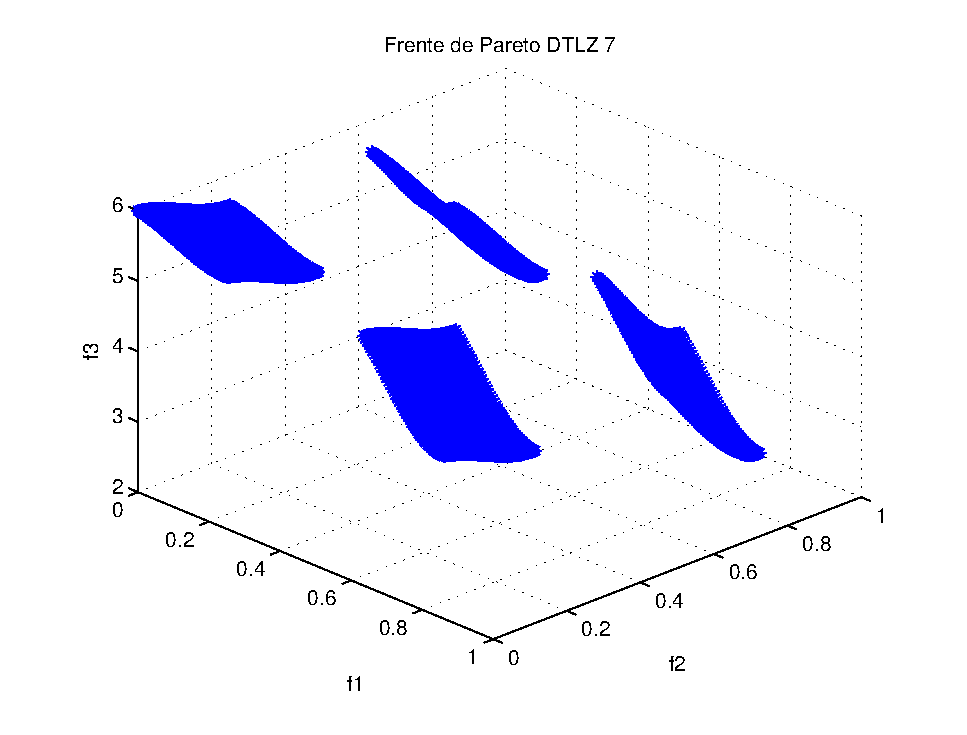
\includegraphics[scale=0.7]{ApendiceA/paretoDTLZ7.eps}
    \caption{Frente de Pareto verdadero de DTLZ7}
    \label{fig:dtlz7}
\end{figure}

\section{Evaluaci\'on del conjunto de problemas DTLZ}

\begin{table}
  \begin{center}
    \begin{tabular}{|l||c|}
	\hline
	Problema  & Punto de referencia \\ 
	\hline
	\hline
	DTLZ1 & $(1.1,1.1,1.1)$ \\ 
	\hline
	DTLZ2 &  $(1.1,1.1,1.1)$\\
	\hline
	DTLZ3 &  $(5.0,5.0,5.0)$\\
	\hline
	DTLZ4 &  $(1.1,1.1,1.1)$\\
	\hline
	DTLZ5 &  $(1.1,1.1,1.1)$\\
	\hline
	DTLZ6 &  $(1.1,1.1,1.1)$\\
	\hline
	DTLZ7 &  $(1.1,1.1,7.0)$\\
	\hline
  \end{tabular}
  \caption{Puntos de referencia utilizados para el conjunto de problemas DTLZ}
  \label{tab:refdtlz}
\end{center}
\end{table}

\newpage
\begin{table}
 \begin{center}
  \begin{tabular}{|l|cc|cc|} \hline
    & \multicolumn{4}{|c|}{Espaciado} \\ 
	\textbf{Algoritmo} & \textbf{Menor} & \textbf{Mayor} & \textbf{Promedio} & \textbf{Desviaci\'on} \\  \hline \hline
	MOPSOhv &0.026239 & 0.184637 & 0.081790 & 0.045829    \\ 
	MOPSOcd &0.531066 & 1.547502 & 0.974734 & 0.295577   \\ 
	NSGA-II &0.015203 & 0.023959 & 0.019360 & 0.002384   \\  
	SMS-EMOA&0.005793 & 0.012914 & 0.006947 & 0.001461   \\  
	\hline\hline
    & \multicolumn{4}{|c|}{DGI} \\ \hline\hline
	MOPSOhv &0.000617 & 0.035965 & 0.013359 & 0.011381  \\ 
	MOPSOcd &0.145461 & 0.462595 & 0.269641 & 0.080597  \\ 
	NSGA-II &0.000540 & 0.003699 & 0.001261 & 0.001148   \\  
	SMS-EMOA &0.005777 & 0.011575 & 0.006088 & 0.001259  \\  
	\hline\hline
    & \multicolumn{4}{|c|}{Hipervolumen} \\ 
  \hline\hline
	MOPSOhv &0.000000 & 1.290672 & 0.838140 & 0.351522  \\ 
	MOPSOcd &0.000000 & 0.000000 & 0.000000 & 0.000000  \\ 
	NSGA-II &1.244198 & 1.297406 & 1.270538 & 0.016839  \\  
	SMS-EMOA &1.123310 & 1.305100 & 1.295857 & 0.039586  \\  
	\hline\hline
	& \multicolumn{4}{|c|}{\textbf{Cobertura}} \\ \hline\hline 
	\textbf{Algoritmo} & \textbf{MOPSOhv} & \textbf{MOPSOcd} & \textbf{NSGA-II} & \textbf{SMS-EMOA} \\  \hline \hline
	\textbf{MOPSOhv} & ---      & 0.964500 & 0.000000 & 0.000000  \\ 
	\textbf{MOPSOcd} & 0.000000 & ---      &  0.000000  & 0.000000 \\ 
	\textbf{NSGA-II} & 0.838500 & 0.977500 & ---       & 0.039000 \\  
	\textbf{SMS-EMOA}& 0.771000 & 0.911500 & 0.000000  & --- \\  
	\hline
	\end{tabular}
\caption{Resultados correspondientes al problema DTLZ1.}
  \label{tab:dtlz1}
\end{center}
\end{table}

\clearpage
\newpage

\begin{figure}
      \begin{center}
	  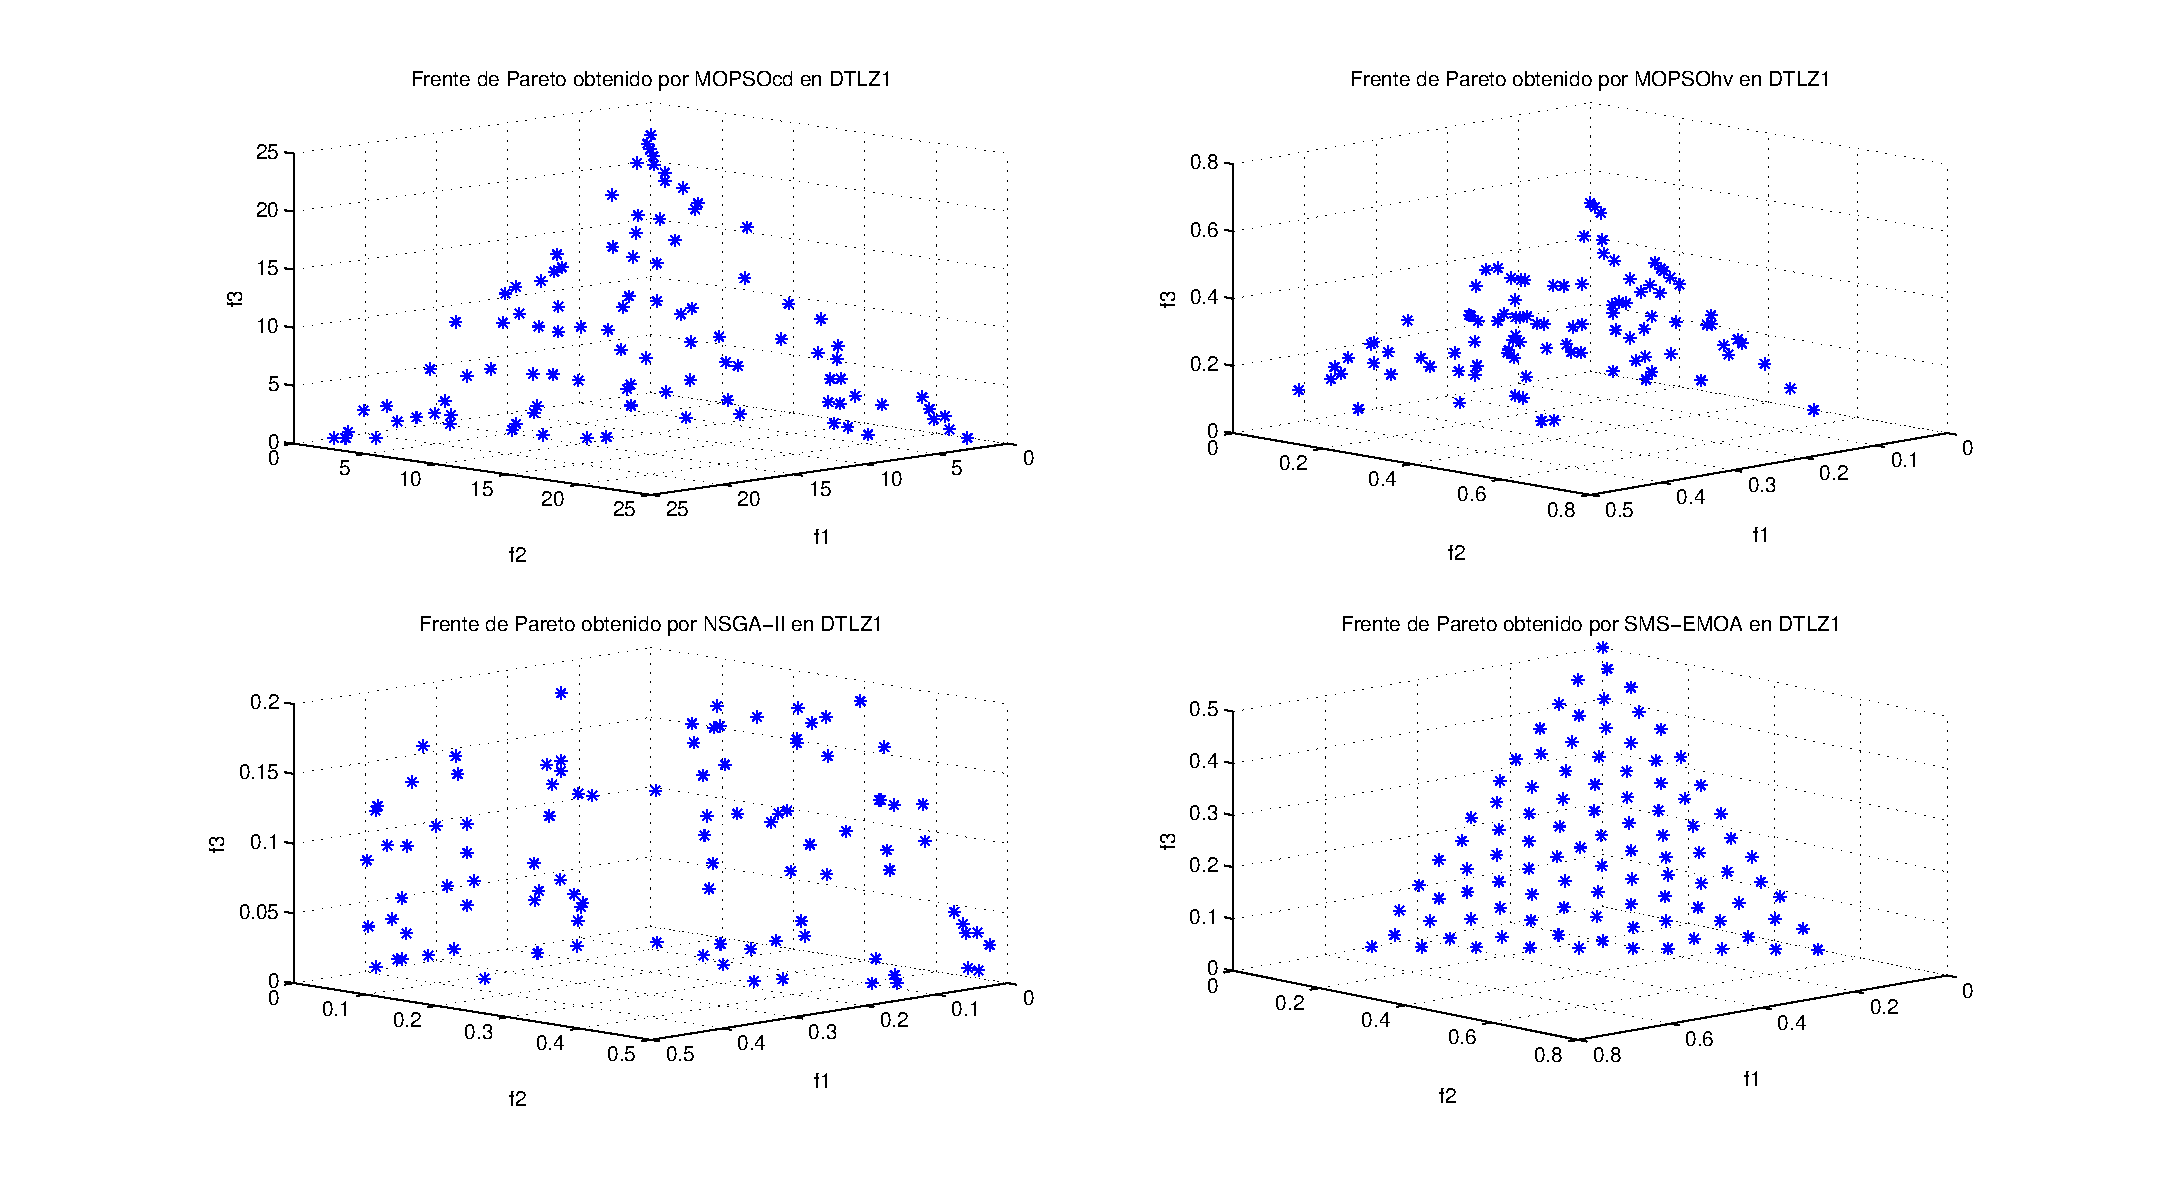
\includegraphics[scale=0.45]{Cap4/rdtlz1r.eps}
      \end{center}
	\caption{Resultados gr\'aficos correspondientes al problema DTLZ1.}
      \label{fig:rDTLZ1}
\end{figure}

\clearpage
\newpage

\begin{table}
 \begin{center}
  \begin{tabular}{|l|cc|cc|} \hline
    & \multicolumn{4}{|c|}{Espaciado} \\ 
	\textbf{Algoritmo} & \textbf{Menor} & \textbf{Mayor} & \textbf{Promedio} & \textbf{Desviaci\'on} \\  \hline \hline
	MOPSOhv &0.031912 & 0.087823 & 0.056173 & 0.012780    \\ 
	MOPSOcd &0.042795 & 0.064965 & 0.052077 & 0.005154  \\ 
	NSGA-II &0.043968 & 0.065239 & 0.055460 & 0.005003   \\  
	SMS-EMOA &0.040210 & 0.047397 & 0.042716 & 0.001942   \\  
	\hline\hline
    & \multicolumn{4}{|c|}{DGI} \\ 
	\hline\hline
	MOPSOhv &0.000421 & 0.003117 & 0.000806 & 0.000611    \\ 
	MOPSOcd &0.000353 & 0.000430 & 0.000383 & 0.000022   \\ 
	NSGA-II &0.000354 & 0.000437 & 0.000380 & 0.000018   \\  
	SMS-EMOA &0.005000 & 0.005000 & 0.005000 & 0.000000   \\  
	\hline\hline
    & \multicolumn{4}{|c|}{Hipervolumen} \\ 
	\hline \hline
	MOPSOhv &0.477781 & 0.695914 & 0.626972 & 0.046583   \\ 
	MOPSOcd &0.637661 & 0.700693 & 0.669615 & 0.019100   \\ 
	NSGA-II &0.676094 & 0.709199 & 0.697212 & 0.007736   \\  
	SMS-EMOA &0.757997 & 0.758163 & 0.758091 & 0.000047   \\  
	\hline\hline
	& \multicolumn{4}{|c|}{\textbf{Cobertura}} \\ \hline\hline 
	\textbf{Algoritmo} & \textbf{MOPSOhv} & \textbf{MOPSOcd} & \textbf{NSGA-II} & \textbf{SMS-EMOA} \\  \hline \hline
	\textbf{MOPSOhv} & ---       & 0.225500  &  0.009000 & 0.000000 \\ 
	\textbf{MOPSOcd} &  0.000000 & ---       & 0.001500  & 0.000000  \\ 
	\textbf{NSGA-II} & 0.001000  &  0.296000 & ---       & 0.010000 \\  
	\textbf{SMS-EMOA}& 0.003000  & 0.444000  &  0.006000 & --- \\  
	\hline
	\end{tabular}
\caption{Resultados correspondientes al problema DTLZ2.}
  \label{tab:dtlz2}
\end{center}
\end{table}

\clearpage
\newpage

\begin{figure}
      \begin{center}
	  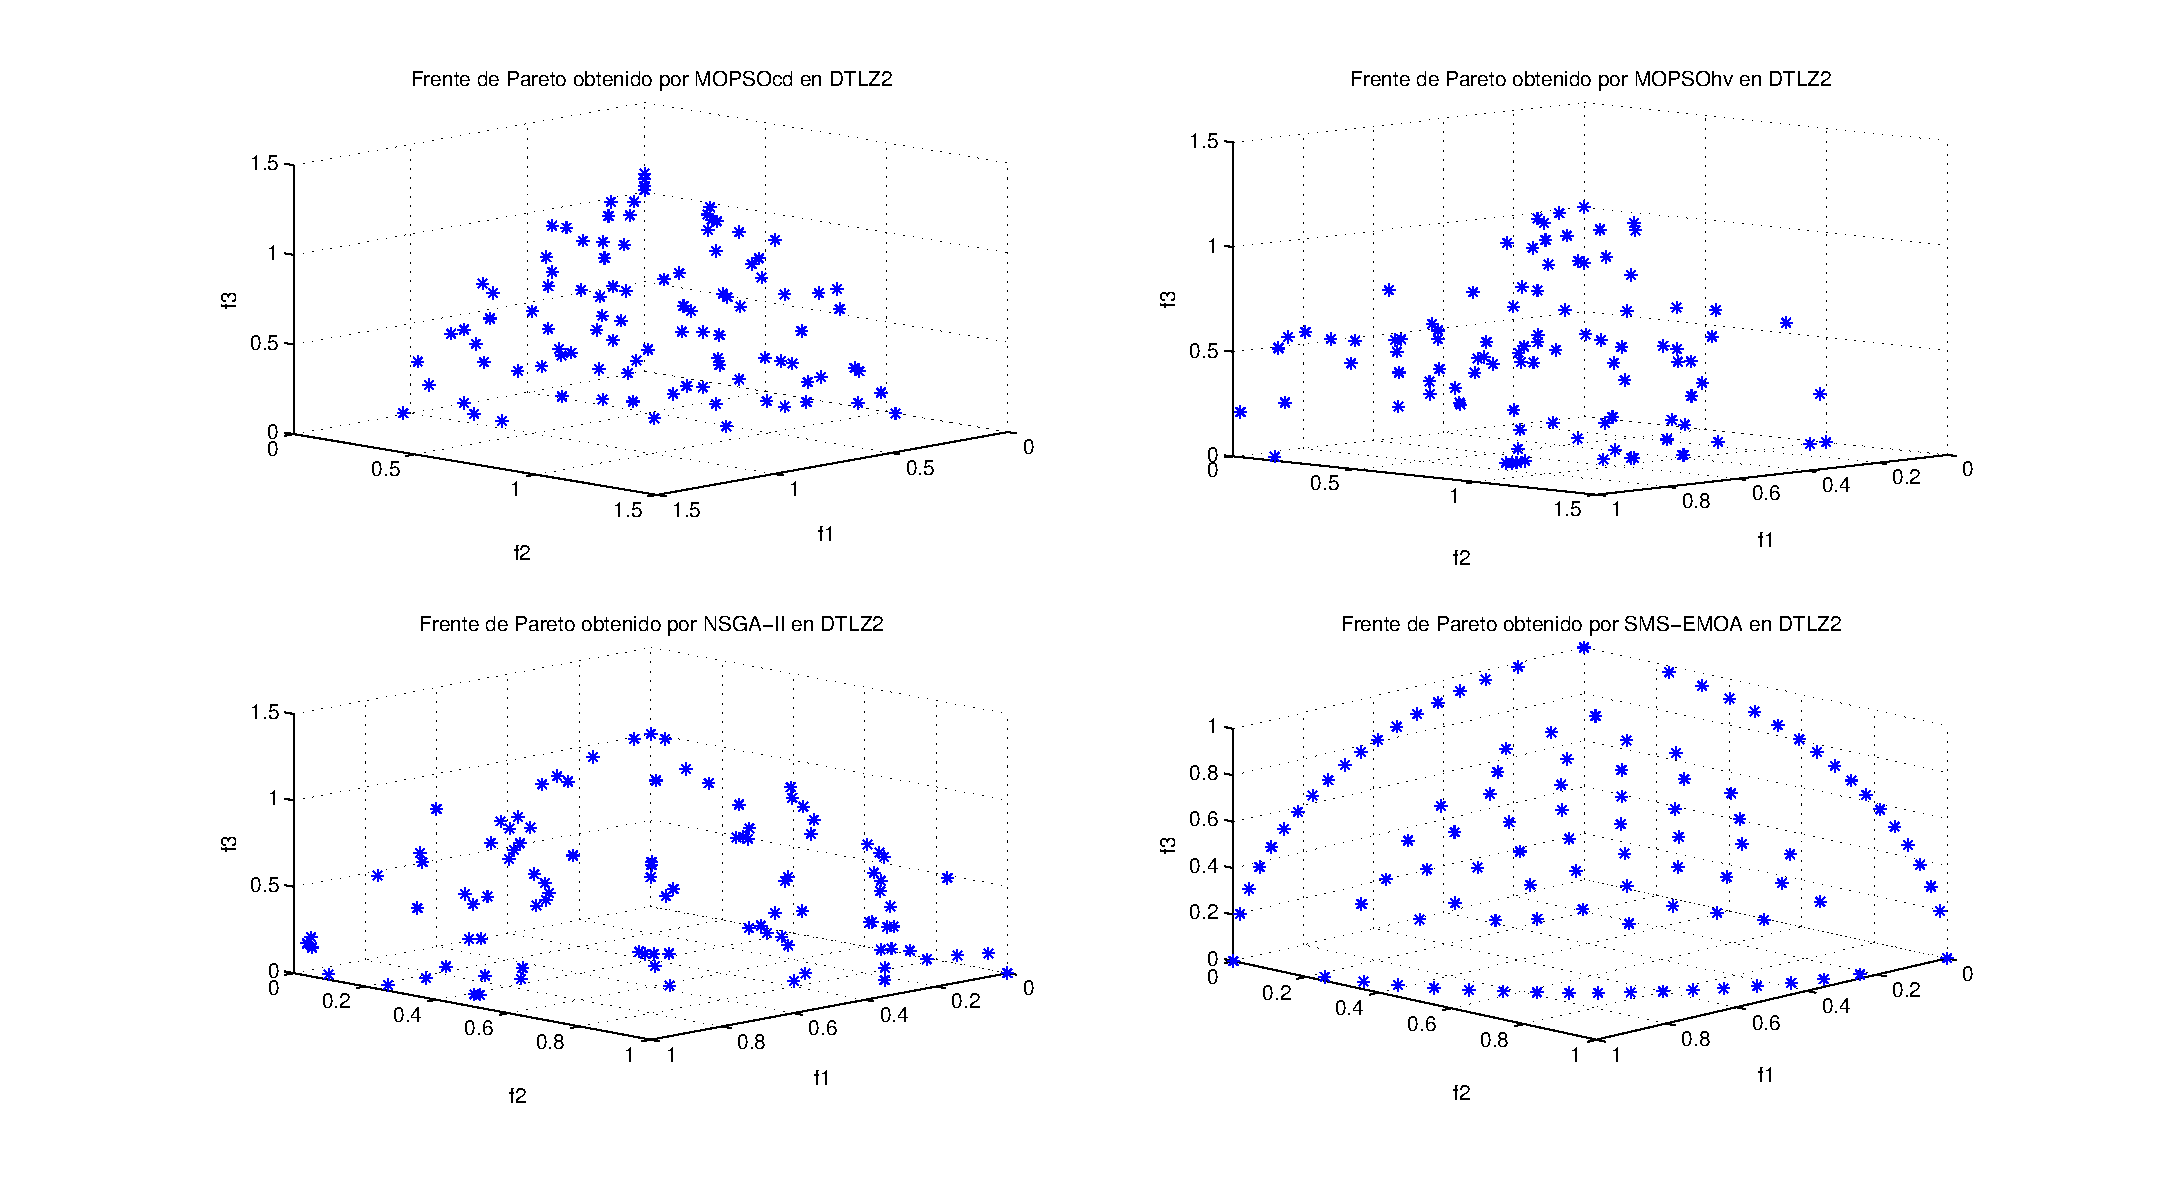
\includegraphics[scale=0.45]{Cap4/rdtlz2r.eps}
      \end{center}
	\caption{Resultados gr\'aficos correspondientes al problema DTLZ2.}
      \label{fig:rDTLZ2}
      \end{figure}

      \clearpage
      \newpage
 
\begin{table}
 \begin{center}
  \begin{tabular}{|l|cc|cc|} \hline
    & \multicolumn{4}{|c|}{Espaciado} \\ 
	\textbf{Algoritmo} & \textbf{Menor} & \textbf{Mayor} & \textbf{Promedio} & \textbf{Desviaci\'on} \\  \hline \hline
	MOPSOhv &0.523852 & 6.539527 & 1.759328 & 1.322038    \\ 
	MOPSOcd &0.774392 & 5.346362 & 2.143857 & 0.915538   \\ 
	NSGA-II &0.045404 & 0.067297 & 0.056032 & 0.004531   \\  
	SMS-EMOA &0.037710 & 0.083937 & 0.043889 & 0.009394  \\  
	\hline\hline
    & \multicolumn{4}{|c|}{DGI} \\ 
	\hline\hline
	MOPSOhv &0.187750 & 1.484958 & 0.594644 & 0.302257   \\ 
	MOPSOcd &0.199480 & 1.812156 & 0.630432 & 0.323953  \\ 
	NSGA-II &0.001123 & 0.001441 & 0.001235 & 0.000083 \\  
	SMS-EMOA &0.015616 & 0.031270 & 0.016425 & 0.003406  \\  
	\hline\hline
    & \multicolumn{4}{|c|}{Hipervolumen} \\ 
	\hline\hline
	MOPSOhv &0.000000 & 0.000000 & 0.000000 & 0.000000 \\ 
	MOPSOcd &0.000000 & 0.000000 & 0.000000 & 0.000000  \\ 
	NSGA-II &123.004398 & 124.174476 & 123.673815 & 0.295556 \\  
	SMS-EMOA &120.390195 & 124.425951 & 124.221079 & 0.878873  \\  
	\hline\hline
	& \multicolumn{4}{|c|}{\textbf{Cobertura}} \\ \hline\hline 
	\textbf{Algoritmo} & \textbf{MOPSOhv} & \textbf{MOPSOcd} & \textbf{NSGA-II} & \textbf{SMS-EMOA} \\  \hline \hline
	\textbf{MOPSOhv} &---       & 0.546000 & 0.000000   & 0.000000  \\ 
	\textbf{MOPSOcd} & 0.215500 & ---      & 0.000000 & 0.000000 \\ 
	\textbf{NSGA-II} & 1.000000 & 0.980000 & ---        & 0.052000 \\  
	\textbf{SMS-EMOA}& 0.960000 & 0.940000 & 0.000000   & --- \\  
	\hline
	\end{tabular}
\caption{Resultados correspondientes al problema DTLZ3.}
  \label{tab:dtlz3}
\end{center}
\end{table}
\clearpage
\newpage

\begin{figure}
      \begin{center}
	  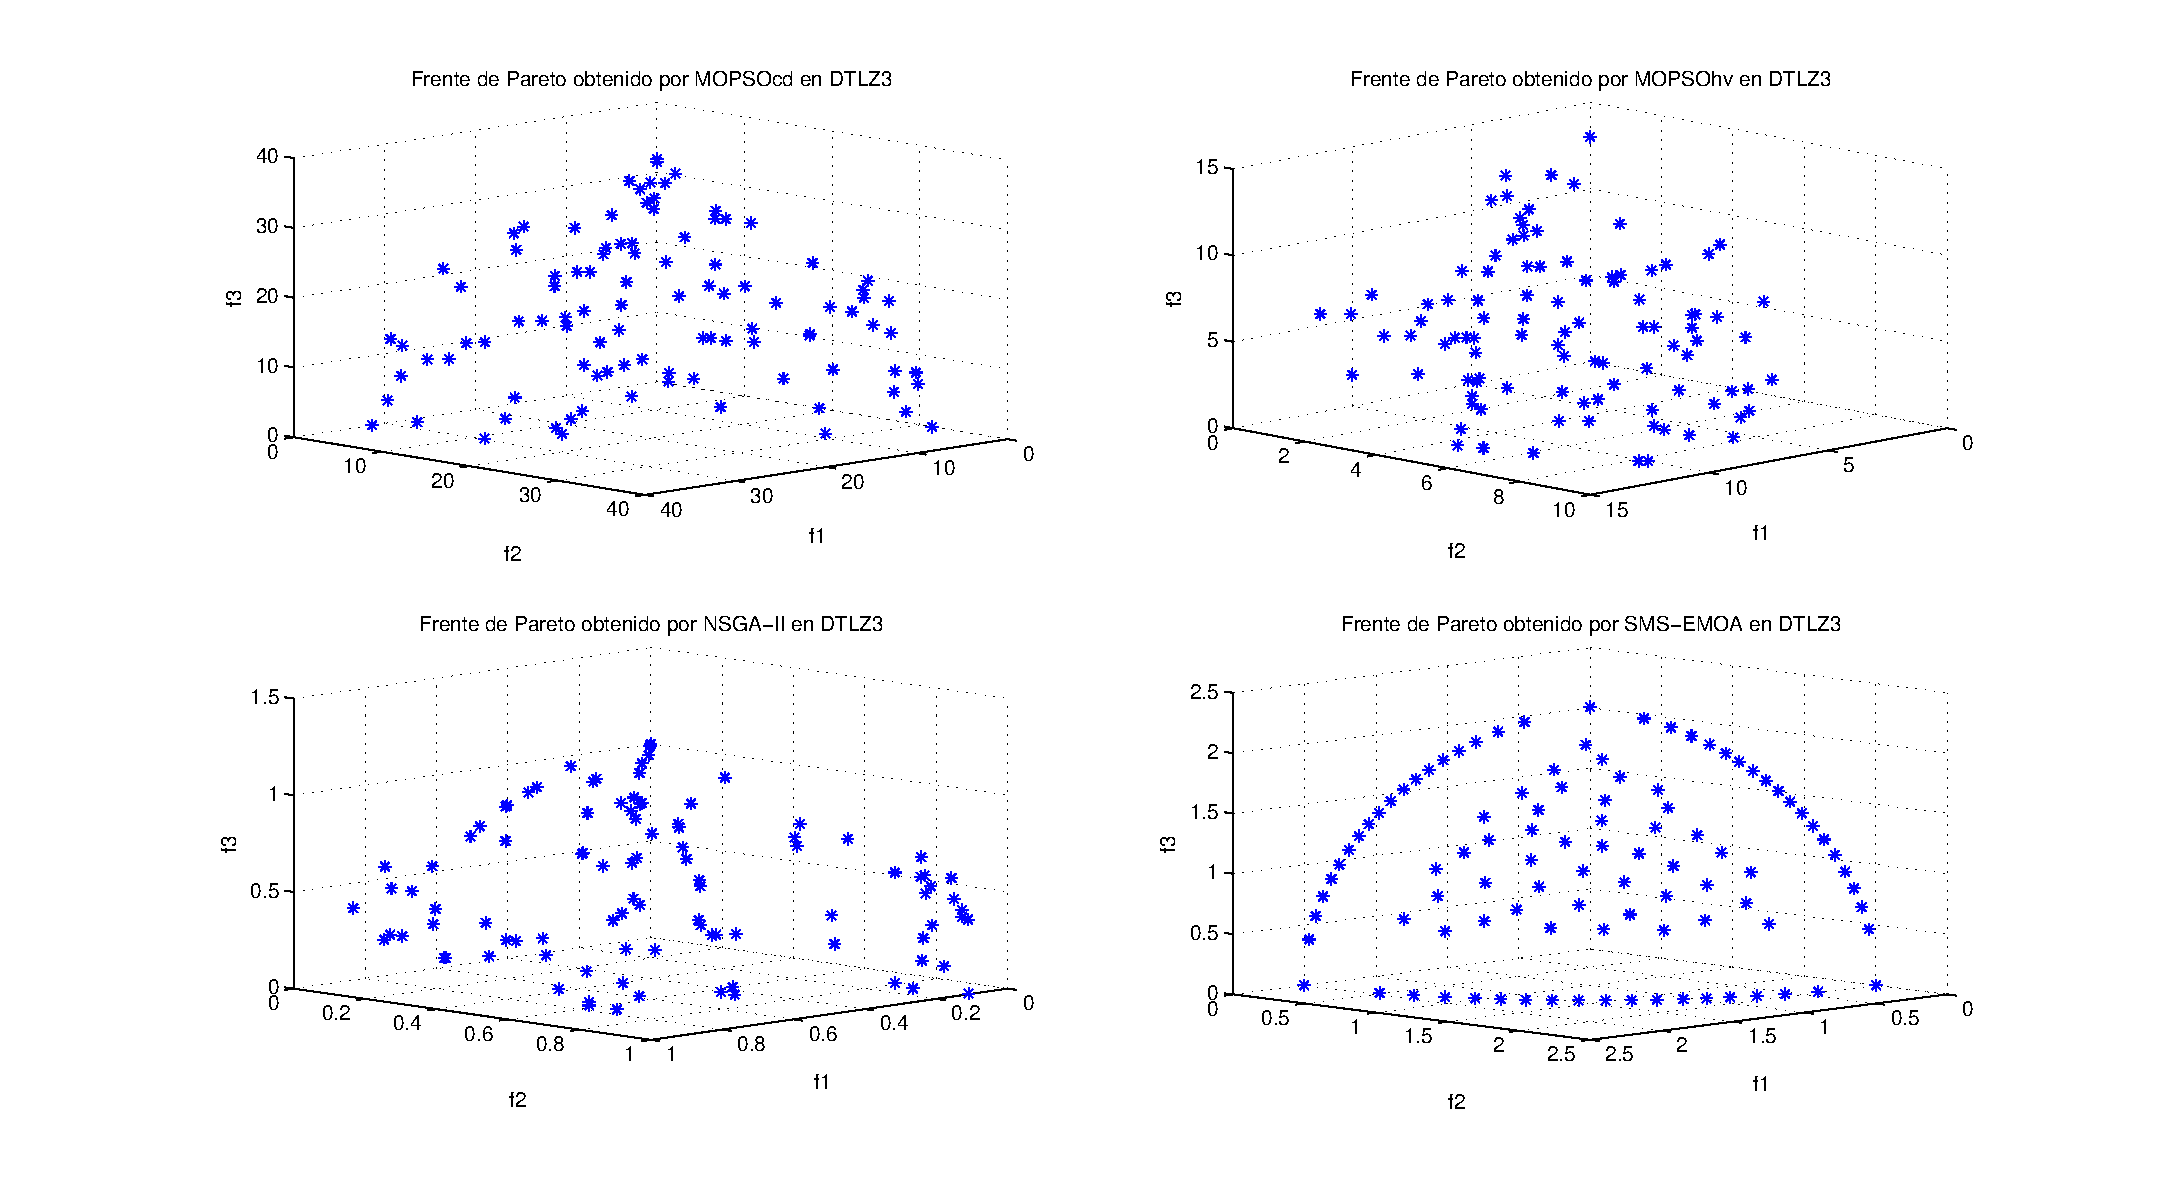
\includegraphics[scale=0.45]{Cap4/rdtlz3r.eps}
      \end{center}
	\caption{Resultados gr\'aficos correspondientes al problema DTLZ3.}
      \label{fig:rDTLZ3}
      \end{figure}

      \clearpage
      \newpage
 

\begin{table}
 \begin{center}
  \begin{tabular}{|l|cc|cc|} \hline
    & \multicolumn{4}{|c|}{Espaciado} \\ 
	\textbf{Algoritmo} & \textbf{Menor} & \textbf{Mayor} & \textbf{Promedio} & \textbf{Desviaci\'on} \\  \hline \hline
	MOPSOhv &0.009443 & 0.080015 & 0.047999 & 0.021016    \\ 
	MOPSOcd &0.052363 & 0.061539 & 0.056542 & 0.002922  \\ 
	NSGA-II &0.000000 & 0.063012 & 0.051862 & 0.013087   \\  
	SMS-EMOA & 0.039215 & 0.045833 & 0.042030 & 0.001928   \\  
	\hline\hline
    & \multicolumn{4}{|c|}{DGI} \\ 
	\hline\hline
	MOPSOhv &0.003982 & 0.010549 & 0.006694 & 0.002366   \\ 
	MOPSOcd &0.001142 & 0.001271 & 0.001208 & 0.000037 \\ 
	NSGA-II &0.001097 & 0.015257 & 0.001875 & 0.003071   \\  
	SMS-EMOA &0.015606 & 0.015606 & 0.015606 & 0.000000   \\  
	\hline\hline
    & \multicolumn{4}{|c|}{Hipervolumen} \\ 
	\hline \hline
	MOPSOhv &0.337305 & 0.666145 & 0.548703 & 0.117426 \\ 
	MOPSOcd &0.668445 & 0.708459 & 0.688920 & 0.010033  \\ 
	NSGA-II &0.121000 & 0.715370 & 0.674632 & 0.127135  \\  
	SMS-EMOA &0.757966 & 0.758160 & 0.758069 & 0.000050   \\  
	\hline\hline
	& \multicolumn{4}{|c|}{\textbf{Cobertura}} \\ \hline\hline 
	\textbf{Algoritmo} & \textbf{MOPSOhv} & \textbf{MOPSOcd} & \textbf{NSGA-II} & \textbf{SMS-EMOA} \\  \hline \hline
	\textbf{MOPSOhv} &---       & 0.189000   & 0.013500   &  0.017000 \\ 
	\textbf{MOPSOcd} & 0.000000  & ---       & 0.000500   &  0.000000   \\ 
	\textbf{NSGA-II} & 0.008421  & 0.199500  & ---       &  0.000000  \\  
	\textbf{SMS-EMOA}&  0.000000 & 0.275500  & 0.009500 & --- \\  
	\hline
	\end{tabular}
\caption{Resultados correspondientes al problema DTLZ4.}
  \label{tab:dtlz4}
\end{center}
\end{table}

\clearpage
\newpage

\begin{figure}
      \begin{center}
	  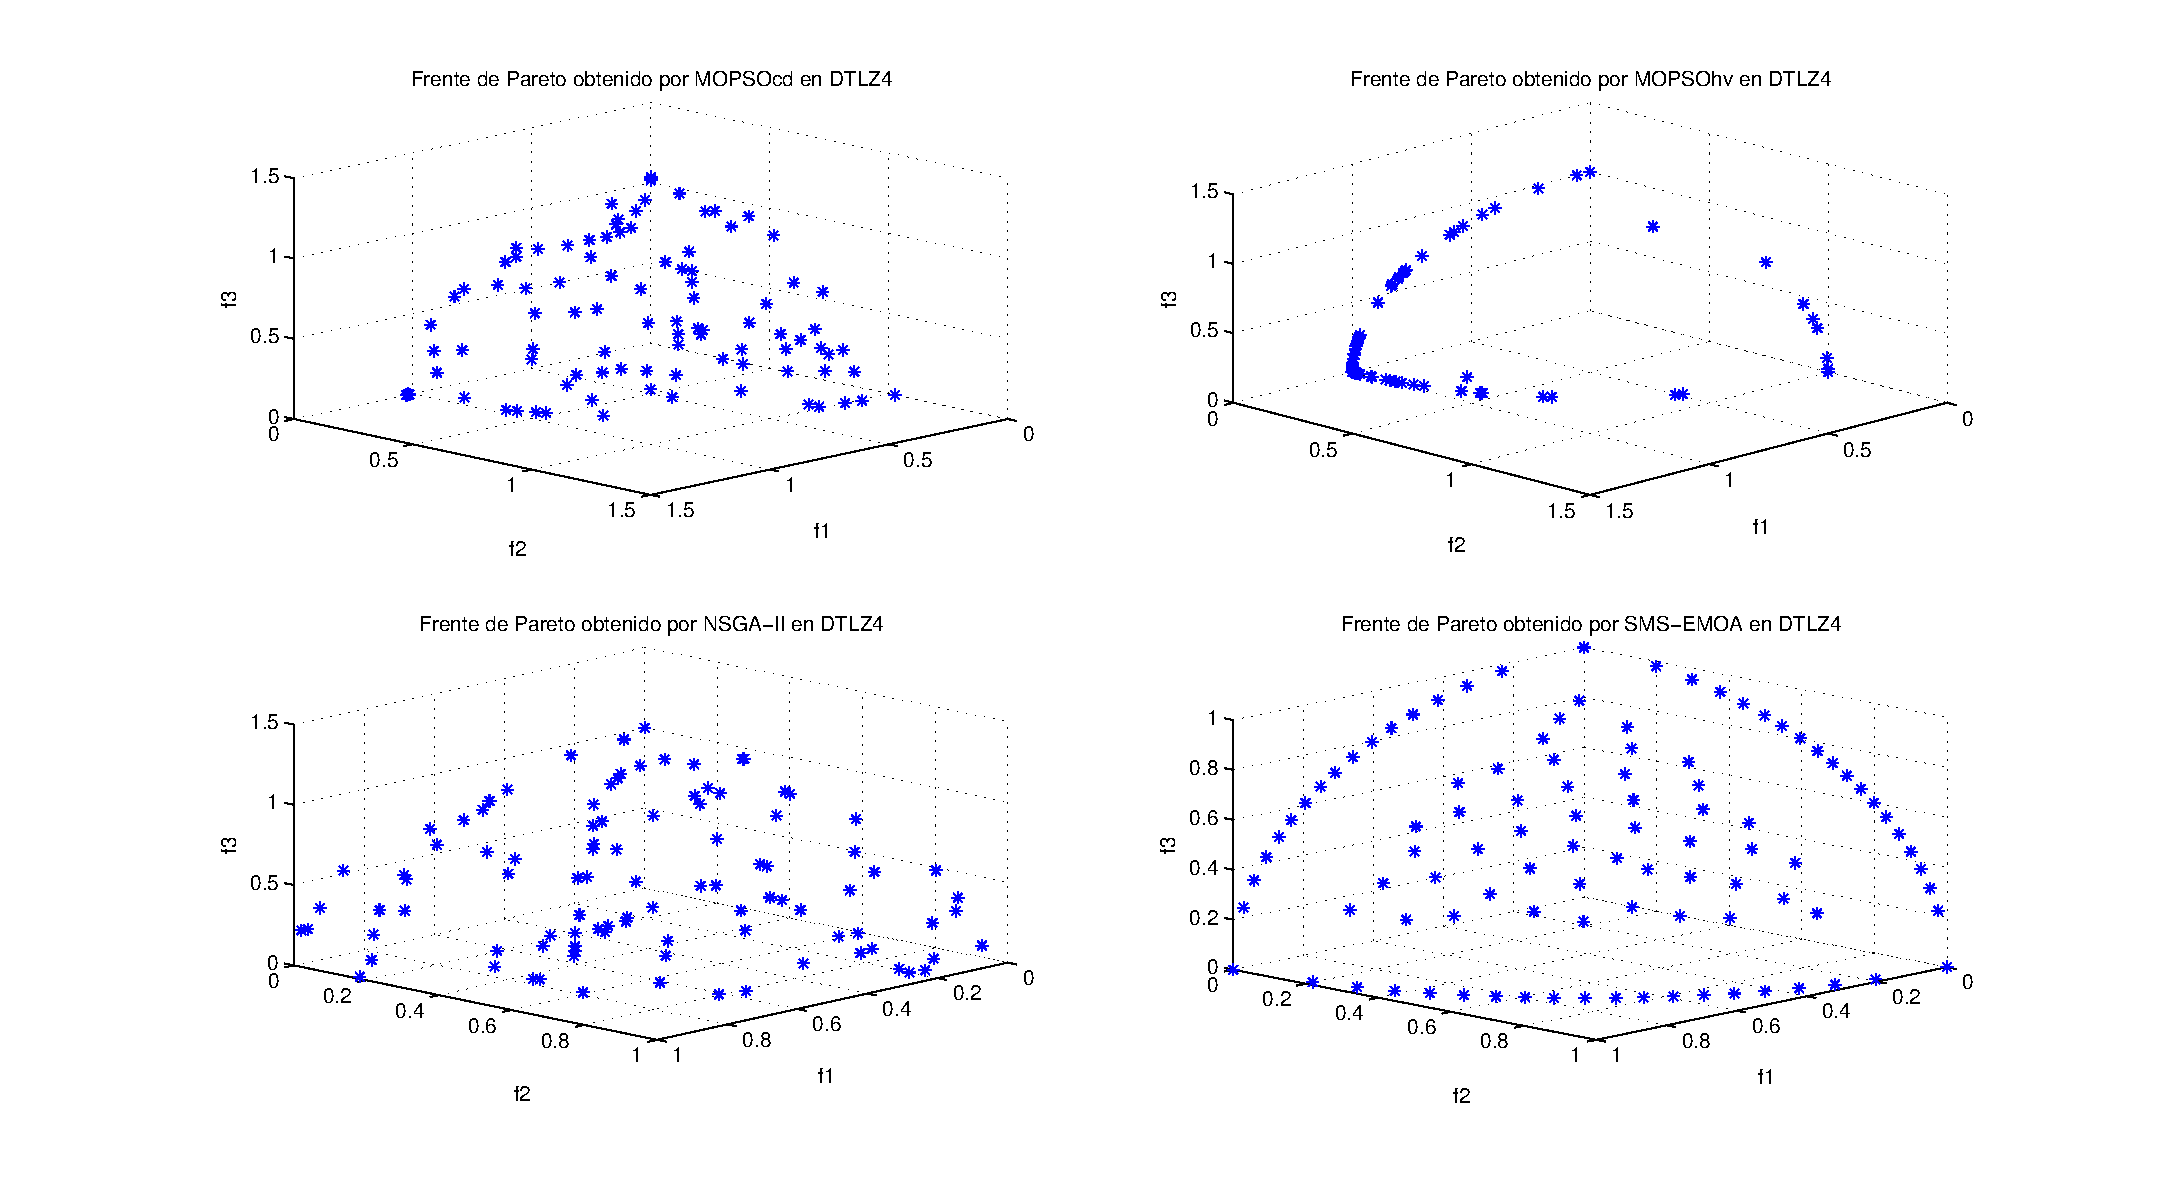
\includegraphics[scale=0.45]{Cap4/rdtlz4r.eps}
      \end{center}
	\caption{Resultados gr\'aficos correspondientes al problema DTLZ4.}
      \label{fig:rDTLZ4}
   \end{figure}

   \clearpage
   \newpage

\begin{table}
 \begin{center}
  \begin{tabular}{|l|cc|cc|} \hline
    & \multicolumn{4}{|c|}{Espaciado} \\ 
	\textbf{Algoritmo} & \textbf{Menor} & \textbf{Mayor} & \textbf{Promedio} & \textbf{Desviaci\'on} \\  \hline \hline
	MOPSOhv &0.009066 & 0.027088 & 0.016552 & 0.005419   \\ 
	MOPSOcd &0.007105 & 0.009411 & 0.008436 & 0.000610   \\ 
	NSGA-II &0.008281 & 0.011557 & 0.009727 & 0.000757  \\  
	SMS-EMOA &0.008044 & 0.009672 & 0.008763 & 0.000463  \\  
	\hline\hline
    & \multicolumn{4}{|c|}{DGI} \\ 
	\hline\hline
	MOPSOhv &0.000125 & 0.001589 & 0.000439 & 0.000390   \\ 
	MOPSOcd &0.000049 & 0.000058 & 0.000054 & 0.000002 \\ 
	NSGA-II &0.000061 & 0.000083 & 0.000069 & 0.000005   \\  
	SMS-EMOA &0.009901 & 0.009901 & 0.009901 & 0.000000   \\  
	\hline
    & \multicolumn{4}{|c|}{Hipervolumen} \\ 
	\hline\hline
	MOPSOhv &0.396024 & 0.435369 & 0.428426 & 0.010028   \\ 
	MOPSOcd &0.438762 & 0.438946 & 0.438852 & 0.000056  \\ 
	NSGA-II &0.437414 & 0.438274 & 0.437990 & 0.000223  \\  
	SMS-EMOA &0.439348 & 0.439390 & 0.439374 & 0.000011   \\  
	\hline\hline
	& \multicolumn{4}{|c|}{\textbf{Cobertura}} \\ \hline\hline 
	\textbf{Algoritmo} & \textbf{MOPSOhv} & \textbf{MOPSOcd} & \textbf{NSGA-II} & \textbf{SMS-EMOA} \\  \hline \hline
	\textbf{MOPSOhv} &---       & 0.024500   &   0.024500  &  0.000000   \\ 
	\textbf{MOPSOcd} & 0.006500 & ---        &  0.034500 &  0.010000 \\ 
	\textbf{NSGA-II} & 0.020500 &  0.000000  & ---       & 0.010000  \\  
	\textbf{SMS-EMOA}& 0.000500 &  0.000000  & 0.022000  & --- \\  
	\hline

	\end{tabular}
\caption{Resultados correspondientes al problema DTLZ5.}
  \label{tab:dtlz5}
\end{center}
\end{table}
\clearpage
\newpage
 \begin{figure}
      \begin{center}
	  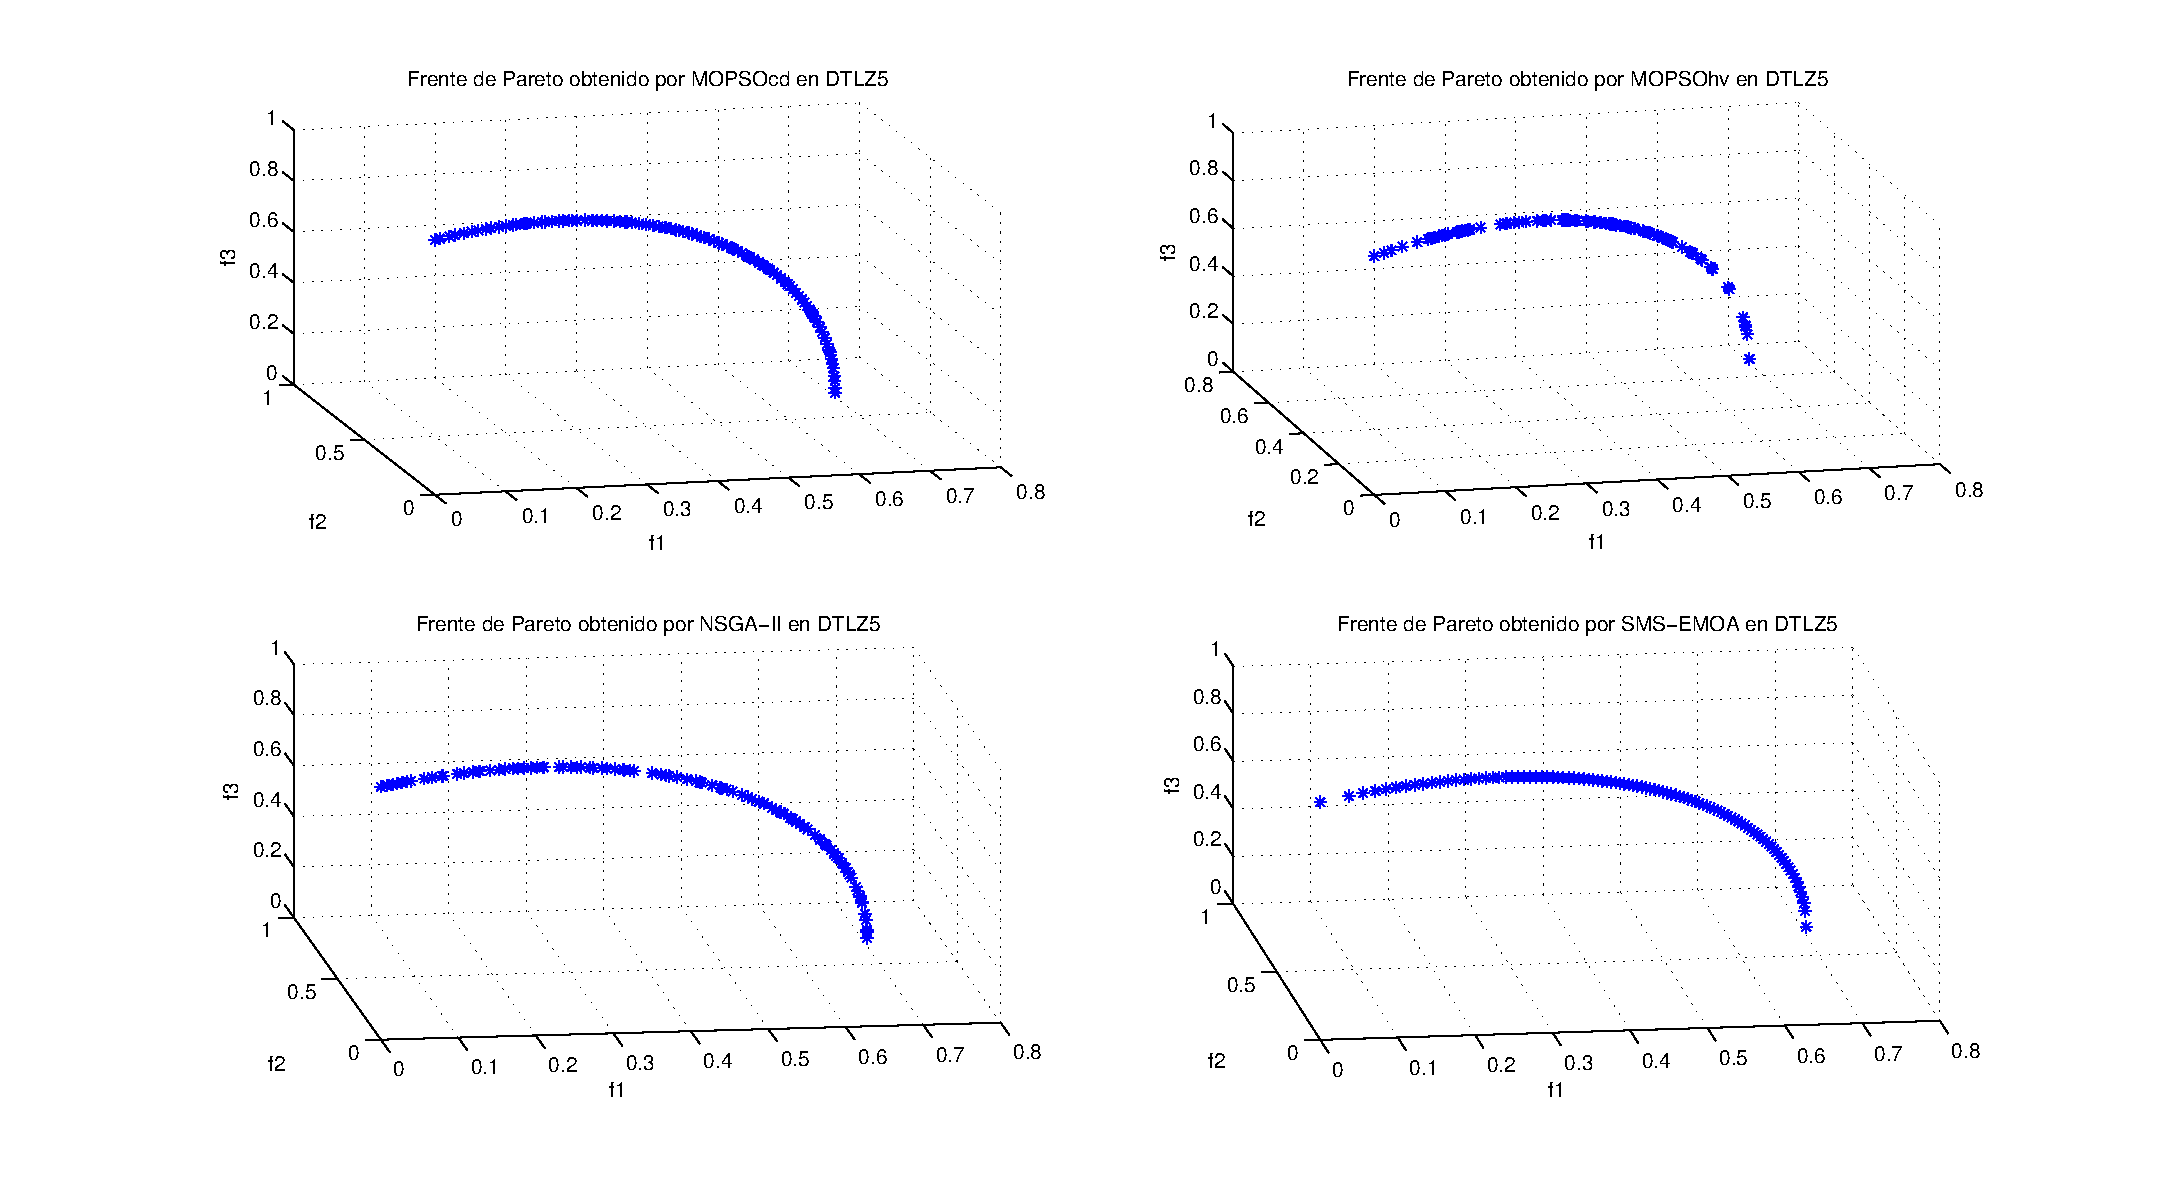
\includegraphics[scale=0.45]{Cap4/rdtlz5r.eps}
      \end{center}
	\caption{Resultados gr\'aficos correspondientes al problema DTLZ5.}
      \label{fig:rDTLZ5}
 \end{figure}
\clearpage
 \newpage
\begin{table}
 \begin{center}
  \begin{tabular}{|l|cc|cc|} \hline
    & \multicolumn{4}{|c|}{Espaciado} \\ 
	\textbf{Algoritmo} & \textbf{Menor} & \textbf{Mayor} & \textbf{Promedio} & \textbf{Desviaci\'on} \\  \hline \hline
	MOPSOhv &0.128037 & 0.220886 & 0.158278 & 0.026187   \\ 
	MOPSOcd &0.271101 & 0.501514 & 0.343938 & 0.052728   \\ 
	NSGA-II &0.011479 & 0.029482 & 0.020970 & 0.004354   \\  
	SMS-EMOA & 0.009705 & 0.020519 & 0.013185 & 0.002414   \\  
	\hline\hline
    & \multicolumn{4}{|c|}{DGI} \\ 
	\hline\hline
	MOPSOhv &0.007386 & 0.015926 & 0.009931 & 0.002293  \\ 
	MOPSOcd &0.009901 & 0.062068 & 0.036889 & 0.012547  \\ 
	NSGA-II &0.000083 & 0.001194 & 0.000648 & 0.000236   \\  
	SMS-EMOA &0.010475 & 0.011392 & 0.010786 & 0.000231  \\  
	\hline\hline
    & \multicolumn{4}{|c|}{Hipervolumen} \\ 
	\hline\hline
	MOPSOhv &0.000000 & 0.000616 & 0.000391 & 0.000277    \\ 
	MOPSOcd &0.000000 & 0.000000 & 0.000000 & 0.000000  \\ 
	NSGA-II &0.303244 & 0.437448 & 0.361529 & 0.028920  \\  
	SMS-EMOA &0.282821 & 0.374890 & 0.340557 & 0.024323   \\  
	\hline\hline
	& \multicolumn{4}{|c|}{\textbf{Cobertura}} \\ \hline\hline 
	\textbf{Algoritmo} & \textbf{MOPSOhv} & \textbf{MOPSOcd} & \textbf{NSGA-II} & \textbf{SMS-EMOA} \\  \hline \hline
	\textbf{MOPSOhv} & --- &  0.920000       & 0.000000  & 0.000000 \\ 
	\textbf{MOPSOcd} & 0.000000 & ---       &  0.000000 &  0.000000  \\ 
	\textbf{NSGA-II} & 0.958000 & 0.996000  & ---       & 0.479500  \\  
	\textbf{SMS-EMOA}& 0.630000 &  0.640000 & 0.001500  & --- \\  
	\hline
	\end{tabular}
\caption{Resultados correspondientes al problema DTLZ6.}
  \label{tab:dtlz6}
\end{center}
\end{table}

\clearpage
\newpage
\begin{figure}
      \begin{center}
	  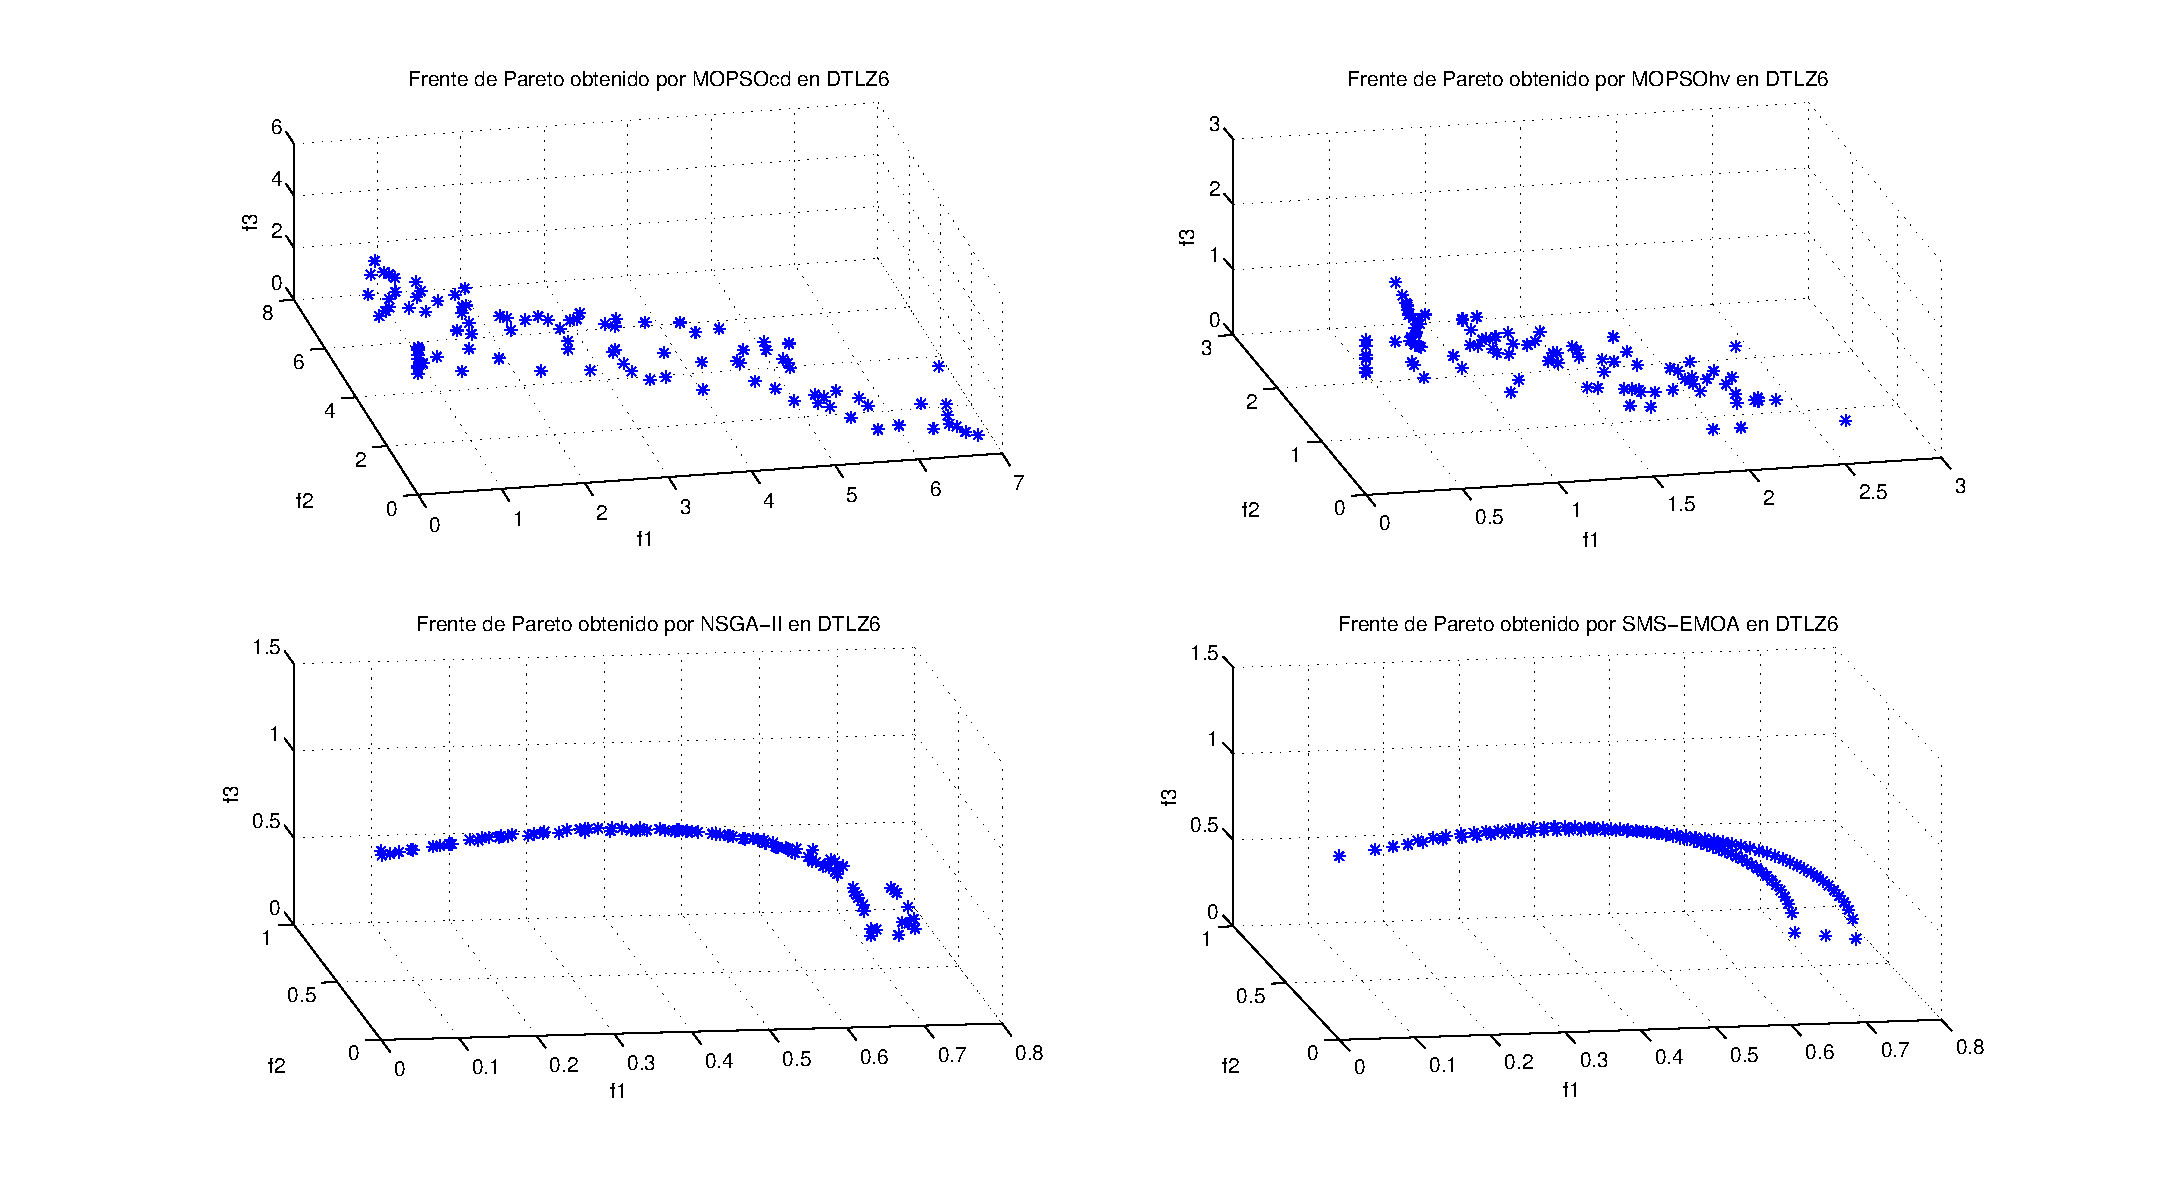
\includegraphics[scale=0.45]{Cap4/rdtlz6r.eps}
      \end{center}
	\caption{Resultados gr\'aficos correspondientes al problema DTLZ6.}
      \label{fig:rDTLZ6}
      \end{figure}
\clearpage
\newpage

 \begin{table}
 \begin{center}
 \begin{tabular}{|l|cc|cc|} \hline
    & \multicolumn{4}{|c|}{Espaciado} \\ 
	\textbf{Algoritmo} & \textbf{Menor} & \textbf{Mayor} & \textbf{Promedio} & \textbf{Desviaci\'on} \\  \hline \hline
	MOPSOhv &0.029933 & 0.140179 & 0.085100 & 0.025882    \\ 
	MOPSOcd & 0.063885 & 0.453648 & 0.114527 & 0.112693   \\ 
	NSGA-II &0.043496 & 0.085744 & 0.068548 & 0.009758  \\  
	SMS-EMOA &0.044055 & 0.063838 & 0.057420 & 0.005603    \\  
	\hline
    & \multicolumn{4}{|c|}{DGI} \\ 
	\hline\hline
	MOPSOhv &0.001446 & 0.005356 & 0.002800 & 0.001392   \\ 
	MOPSOcd & 0.001228 & 0.002112 & 0.001558 & 0.000205   \\ 
	NSGA-II & 0.000802 & 0.005285 & 0.001123 & 0.000957  \\  
	SMS-EMOA &0.013925 & 0.021469 & 0.015064 & 0.002691  \\  
	\hline\hline
    & \multicolumn{4}{|c|}{Hipervolumen} \\ 
	\hline\hline
	MOPSOhv & 2.359510 & 2.812829 & 2.608814 & 0.123164  \\ 
	MOPSOcd & 2.430821 & 2.744141 & 2.648845 & 0.072522   \\ 
	NSGA-II & 2.578211 & 3.011594 & 2.974631 & 0.091615   \\  
	SMS-EMOA &5.055289 & 5.528637 & 5.456793 & 0.168653   \\  
	\hline\hline	
	& \multicolumn{4}{|c|}{\textbf{Cobertura}} \\ \hline\hline 
	\textbf{Algoritmo} & \textbf{MOPSOhv} & \textbf{MOPSOcd} & \textbf{NSGA-II} & \textbf{SMS-EMOA} \\  \hline \hline
	\textbf{MOPSOhv} &---       & 0.460000   & 0.061500 &  0.00000	 \\ 
	\textbf{MOPSOcd} & 0.003000 & ---       &  0.000000  & 0.000000 \\ 
	\textbf{NSGA-II} & 0.008000 & 0.658500  & ---      &  0.000000    \\  
	\textbf{SMS-EMOA}& 0.940000 & 0.890000  & 0.980000 & --- \\  
	\hline	
	\end{tabular}
\caption{Resultados correspondientes al problema DTLZ7.}
  \label{tab:dtlz7}
\end{center}
\end{table}

\clearpage
\newpage

\begin{figure}
      \begin{center}
	  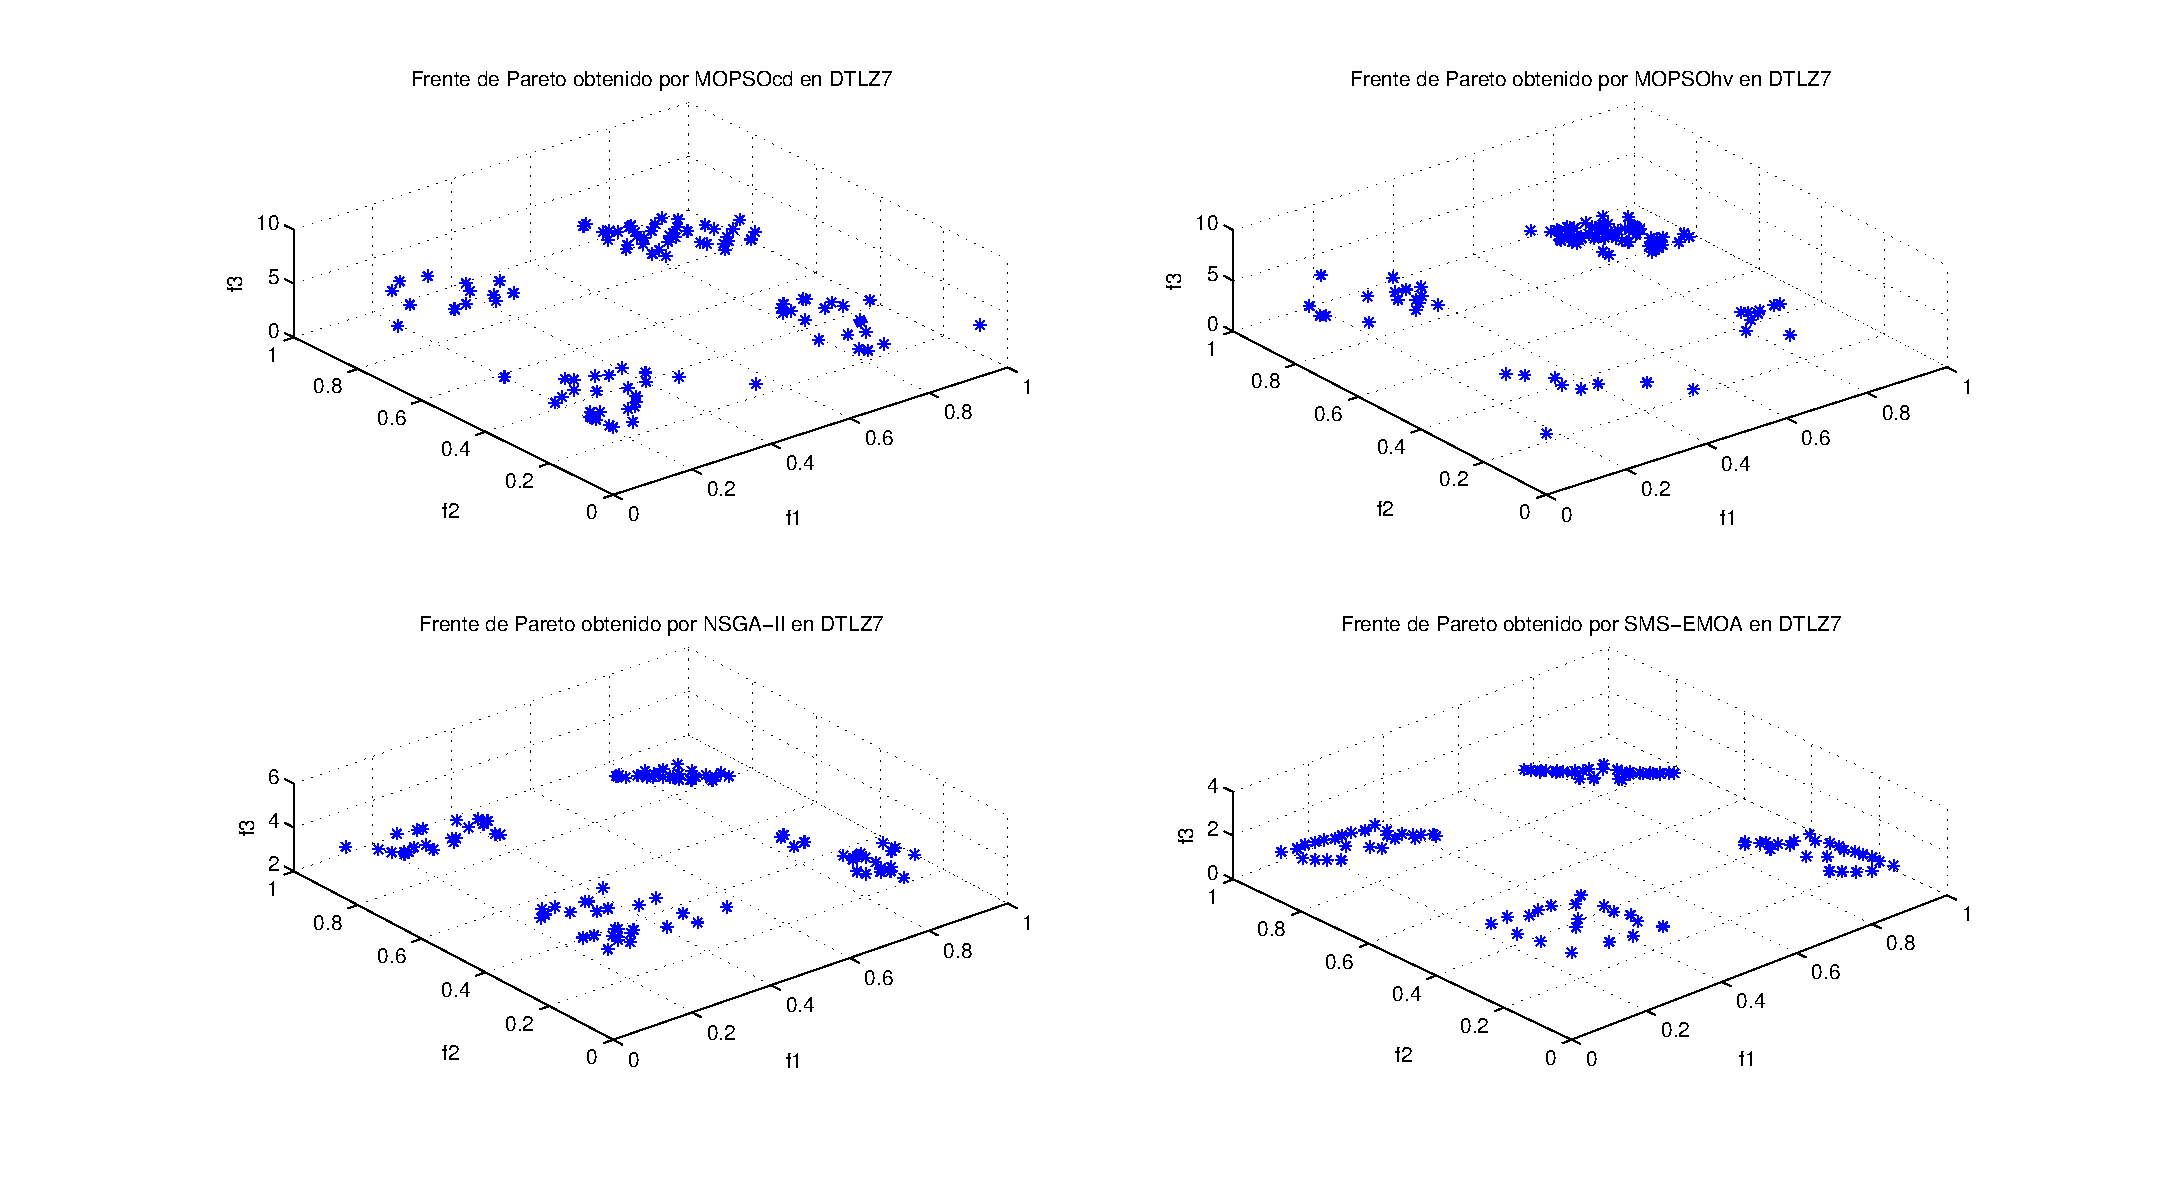
\includegraphics[scale=0.45]{Cap4/rdtlz7r.eps}
      \end{center}
	\caption{Resultados gr\'aficos correspondientes al problema DTLZ7.}
      \label{fig:rDTLZ7}
      \end{figure}
\clearpage

Para calcular la m\'etrica del hipervolumen se utiliza como punto de referencia el mostrado en la tabla \ref{tab:refdtlz}.
Los resultados obtenidos por nuestra propuesta para los problemas DTLZ3 y DTLZ6 son mejores que los obtenidos por el MOPSOcd,
ya que las soluciones de nuestra propuesta dominan completamente las soluciones arrojadas por MOPSOcd. 
Sin embargo, los resultados de nuestra propuesta son malos en comparaci\'on con los obtenidos por SMS-EMOA y NSGA-II, los cuales 
obtuvieron soluciones que dominan completamente a las nuestras (tablas \ref{tab:dtlz1}, \ref{tab:dtlz3} y \ref{tab:dtlz6}). 

El problema DTLZ4 presenta un frente de Pareto c\'oncavo. Los resultados muestran que nuestra propuesta se distribuyen 
en s\'olo una parte del frente de Pareto (figura \ref{fig:rDTLZ5}). Sin embargo, nuestras soluciones son mejores (en terminos de
convergencia) que los dem\'as algoritmos, excepto por las de SMS-EMOA (tabla \ref{tab:dtlz4}).

El problema DTLZ5 presenta un frente de Pareto curvo. DTLZ5 se considera un problema f\'acil, ya que su espacio de b\'usqueda 
presenta sesgo hacia soluciones cercanas al frente de Pareto verdadero. Los resultados son similares para todos los algoritmos 
(figura \ref{fig:rDTLZ5}). Sin embargo, nuestras soluciones son mejores (en terminos de convergencia) que los dem\'as algoritmos
excepto por las de SMS-EMOA (tabla \ref{tab:dtlz5}).

El problema DTLZ7 presenta un frente de Pareto con regiones discontinuas. Los resultados de nuestra propuesta son similares que los de 
los algoritmos NSGA-II y MOPSOcd (figura \ref{fig:rDTLZ7}). Sin embargo, nuestras soluciones son dominadas por las obtenidas por SMS-EMOA
(tabla \ref{tab:dtlz7}).

\section{Resultados de escalabilidad}

 Se utiliza el problema DTLZ2 para probar la escalabilidad de nuestro algoritmo de dos a diez objetivos. Las soluciones son comparadas con 
 el NSGA-II, MOPSO-cd y el SMS-EMOA. Se realizaron diez ejecuciones independientes, con 100 individuos y 1200 generaciones usando los 
 par\'ametros de las tablas \ref{tab:parametros1}, \ref{tab:parametros2} y \ref{tab:parametros3}. El punto $\vec{1.1}$ es utlizado como 
 referencia para la m\'etrica del hipervolumen.
 
\begin{longtable}{|l|cc|cc|} 
\hline
    & \multicolumn{4}{|c|}{\textbf{2 Objetivos}} \\ 
	\textbf{Algoritmo} & \textbf{Menor} & \textbf{Mayor} & \textbf{Promedio} & \textbf{Desviaci\'on} \\  \hline \hline
	\textbf{MOPSOhv} & 0.006496 & 0.008450 & 0.007529 & 0.000509 \\ 
	\textbf{MOPSOcd} & 0.006508 & 0.007755 & 0.007165 & 0.000350 \\ 
	\textbf{NSGA-II} & 0.006558 & 0.008114 & 0.007298 & 0.000441 \\  
	\textbf{SMS-EMOA}& 0.007164 & 0.008134 & 0.007687 & 0.000324  \\  
	\hline\hline
    & \multicolumn{4}{|c|}{\textbf{3  Objetivos}} \\ 
	\hline\hline
	\textbf{MOPSOhv} & 0.040552 & 0.075311 & 0.060766 & 0.010465 \\ 
	\textbf{MOPSOcd} & 0.046830 & 0.059367 & 0.052755 & 0.003508 \\ 
	\textbf{NSGA-II} & 0.047551 & 0.062545 & 0.055653 & 0.004653 \\  
	\textbf{SMS-EMOA}& 0.040739 & 0.045160 & 0.042945 & 0.001627 \\
	\hline\hline
    & \multicolumn{4}{|c|}{\textbf{4 Objetivos}} \\ 
	\hline\hline
	\textbf{MOPSOhv} & 0.060814 & 0.103256 & 0.076769 & 0.013224 \\ 
	\textbf{MOPSOcd} & 0.255004 & 0.351009 & 0.307083 & 0.029160 \\ 
	\textbf{NSGA-II} & 0.099124 & 0.121004 & 0.110590 & 0.007367 \\  
	\textbf{SMS-EMOA}& 0.060019 & 0.063409 & 0.061934 & 0.001271 \\ 
	\hline\hline
 & \multicolumn{4}{|c|}{\textbf{5 Objetivos}} \\ 
	\hline\hline
	\textbf{MOPSOhv} & 0.062663 & 0.115829 & 0.096073 & 0.016611    \\ 
	\textbf{MOPSOcd} & 0.357735 & 0.509170 & 0.439317 & 0.048635 \\ 
	\textbf{NSGA-II} & 0.176407 & 0.213365 & 0.194858 & 0.012554  \\  
	\textbf{SMS-EMOA} & --- & --- & --- & --- \\
	\hline\hline
& \multicolumn{4}{|c|}{\textbf{6 Objetivos}} \\ 
	\hline\hline
	\textbf{MOPSOhv} & 0.069909 & 0.146411 & 0.115437 & 0.022606    \\ 
	\textbf{MOPSOcd} & 0.472034 & 0.601704 & 0.536438 & 0.044512 \\ 
	\textbf{NSGA-II} & 0.326463 & 0.462761 & 0.393104 & 0.040260 \\  
	\textbf{SMS-EMOA} & --- & --- & --- & --- \\
	\hline\hline
 & \multicolumn{4}{|c|}{\textbf{7 Objetivos}} \\ 
	\hline\hline
	\textbf{MOPSOhv} & 0.104604 & 0.198331 & 0.134378 & 0.027768   \\ 
	\textbf{MOPSOcd} & 0.567486 & 0.800344 & 0.666199 & 0.064909  \\ 
	\textbf{NSGA-II} & 0.555849 & 0.750226 & 0.626970 & 0.053539 \\  
	\textbf{SMS-EMOA} & --- & --- & --- & --- \\
	\hline\hline
 & \multicolumn{4}{|c|}{\textbf{8 Objetivos}} \\ 
	\hline\hline
	\textbf{MOPSOhv} & 0.091730 & 0.173281 & 0.122761 & 0.025681   \\ 
	\textbf{MOPSOcd} & 0.656487 & 0.898391 & 0.768978 & 0.083783 \\ 
	\textbf{NSGA-II} & 0.707636 & 0.843402 & 0.773139 & 0.048302 \\ 
	\textbf{SMS-EMOA} & --- & --- & --- & --- \\
	\hline\hline
 & \multicolumn{4}{|c|}{\textbf{9 Objetivos}} \\ 
	\hline\hline
	\textbf{MOPSOhv} &0.069848 & 0.150881 & 0.109239 & 0.026673   \\ 
	\textbf{MOPSOcd} & 0.656487 & 0.898391 & 0.768978 & 0.083783 \\ 
	\textbf{NSGA-II} &0.883374 & 0.977749 & 0.913665 & 0.025785 \\ 
	\textbf{SMS-EMOA} & --- & --- & --- & --- \\
	\hline\hline
 & \multicolumn{4}{|c|}{\textbf{10 Objetivos}} \\ 
	\hline\hline
	\textbf{MOPSOhv} &0.090387 & 0.180091 & 0.129630 & 0.028221    \\ 
	\textbf{MOPSOcd} &0.682277 & 0.953287 & 0.826685 & 0.093907  \\ 
	\textbf{NSGA-II} &0.936894 & 1.132359 & 1.032422 & 0.071610\\  
	\textbf{SMS-EMOA} & --- & --- & --- & --- \\
	\hline\hline
\caption{Resultados de la m\'etrica de espaciado para DTLZ2 de 2 a 10 objetivos.}
  \label{tab:dtlz2_es}
\end{longtable}
 
\begin{longtable}{|l|cc|cc|} 
\hline
    & \multicolumn{4}{|c|}{\textbf{2 Objetivos}} \\ 
	\textbf{Algoritmo} & \textbf{Menor} & \textbf{Mayor} & \textbf{Promedio} & \textbf{Desviaci\'on} \\  \hline \hline
	\textbf{MOPSOhv} & 0.420910 & 0.420993 & 0.420962 & 0.000031\\ 
	\textbf{MOPSOcd} & 0.420317 & 0.420437 & 0.420372 & 0.000037\\ 
	\textbf{NSGA-II} & 0.418849 & 0.419966 & 0.419588 & 0.000323\\  
	\textbf{SMS-EMOA}& 0.421020 & 0.421027 & 0.421023 & 0.000003\\  
	\hline\hline
    & \multicolumn{4}{|c|}{\textbf{3  Objetivos}} \\ 
	\hline\hline
	\textbf{MOPSOhv} & 0.597900 & 0.697158 & 0.644946 & 0.030303\\ 
	\textbf{MOPSOcd} & 0.622449 & 0.698677 & 0.667862 & 0.024190\\ 
	\textbf{NSGA-II} & 0.676373 & 0.708493 & 0.697689 & 0.009213\\  
	\textbf{SMS-EMOA}& 0.757991 & 0.758168 & 0.758071 & 0.000056\\
	\hline\hline
    & \multicolumn{4}{|c|}{\textbf{4 Objetivos}} \\ 
	\hline\hline
	\textbf{MOPSOhv} &0.570237 & 0.735955 & 0.649871 & 0.046065 \\ 
	\textbf{MOPSOcd} &0.000000 & 0.000000 & 0.000000 & 0.000000 \\ 
	\textbf{NSGA-II} &0.805413 & 0.876853 & 0.834518 & 0.019843 \\  
	\textbf{SMS-EMOA}&1.044708 & 1.044792 & 1.044734 & 0.000030 \\ 
	\hline\hline
 & \multicolumn{4}{|c|}{\textbf{5 Objetivos}} \\ 
	\hline\hline
	\textbf{MOPSOhv} &0.526935 & 0.821024 & 0.686608 & 0.091850 \\ 
	\textbf{MOPSOcd} &0.000000 & 0.000000 & 0.000000 & 0.000000 \\ 
	\textbf{NSGA-II} &0.624795 & 0.874966 & 0.806271 & 0.075088 \\  
	\textbf{SMS-EMOA}& --- & --- & --- & --- \\
	\hline\hline
& \multicolumn{4}{|c|}{\textbf{6 Objetivos}} \\ 
	\hline\hline
	\textbf{MOPSOhv} &0.588840 & 0.897113 & 0.768027 & 0.106912 \\ 
	\textbf{MOPSOcd} &0.000000 & 0.000000 & 0.000000 & 0.000000 \\ 
	\textbf{NSGA-II} &0.016168 & 0.385332 & 0.195606 & 0.133364 \\  
	\textbf{SMS-EMOA}& --- & --- & --- & --- \\
	\hline\hline
 & \multicolumn{4}{|c|}{\textbf{7 Objetivos}} \\ 
	\hline\hline
	\textbf{MOPSOhv} &0.779870 & 0.986701 & 0.897171 & 0.059289 \\ 
	\textbf{MOPSOcd} &0.000000 & 0.000000 & 0.000000 & 0.000000 \\ 
	\textbf{NSGA-II} &0.000960 & 0.336963 & 0.146724 & 0.119704 \\  
	\textbf{SMS-EMOA} & --- & --- & --- & --- \\
	\hline\hline
 & \multicolumn{4}{|c|}{\textbf{8 Objetivos}} \\ 
	\hline\hline
	\textbf{MOPSOhv} &0.711453 & 1.069716 & 0.923948 & 0.098939 \\ 
	\textbf{MOPSOcd} &0.000000 & 0.000000 & 0.000000 & 0.000000 \\ 
	\textbf{NSGA-II} &0.071442 & 0.358558 & 0.185958 & 0.088435 \\ 
	\textbf{SMS-EMOA} & --- & --- & --- & --- \\
	\hline\hline
 & \multicolumn{4}{|c|}{\textbf{9 Objetivos}} \\ 
	\hline\hline
	\textbf{MOPSOhv} &0.767567 & 1.063881 & 0.894945 & 0.098291 \\ 
	\textbf{MOPSOcd} &0.000000 & 0.000000 & 0.000000 & 0.000000 \\ 
	\textbf{NSGA-II} &0.039463 & 0.397496 & 0.212041 & 0.124973 \\ 
	\textbf{SMS-EMOA} & --- & --- & --- & --- \\
	\hline\hline
 & \multicolumn{4}{|c|}{\textbf{10 Objetivos}} \\ 
	\hline\hline
	\textbf{MOPSOhv} &0.946736 & 1.228404 & 1.080952 & 0.085351   \\ 
	\textbf{MOPSOcd} &0.000000 & 0.000000 & 0.000000 & 0.000000 \\ 
	\textbf{NSGA-II} &0.015169 & 0.440330 & 0.224003 & 0.127577 \\  
	\textbf{SMS-EMOA} & --- & --- & --- & --- \\
	\hline\hline
\caption{Resultados de la m\'etrica de hipervolumen para DTLZ2 con 2 a 10 objetivos.}
  \label{tab:dtlz2_hv}
\end{longtable}

Las tablas \ref{tab:dtlz2_es} y \ref{tab:dtlz2_hv} muestran los resultados obtenidos para 
DTLZ2 con 2 a 10 objetivos. El NSGA-II muestra un deterioro en la 
calidad de las soluciones cuando aumenta el n\'umero de objetivos del problema con un costo 
computacional bajo. El SMS-EMOA muestra tener buenos resultados, pero es muy costoso, computacionalmente hablando. 
MOPSOcd muestra que su desempe\~no no es escalable ya que se degrada r\'apidamente al aumentar el n\'umero de 
funciones objetivo. Nuestra propuesta  muestra tener buenos resultados en la
calidad de las soluciones cuando aumentan el n\'umero de objetivos del problema, manteniendo un costo
computacional razonable, lo que hace a nuestro algoritmo competitivo respecto a los dem\'as (figura \ref{fig:tescala}).

  \begin{figure}
      \begin{center}
	  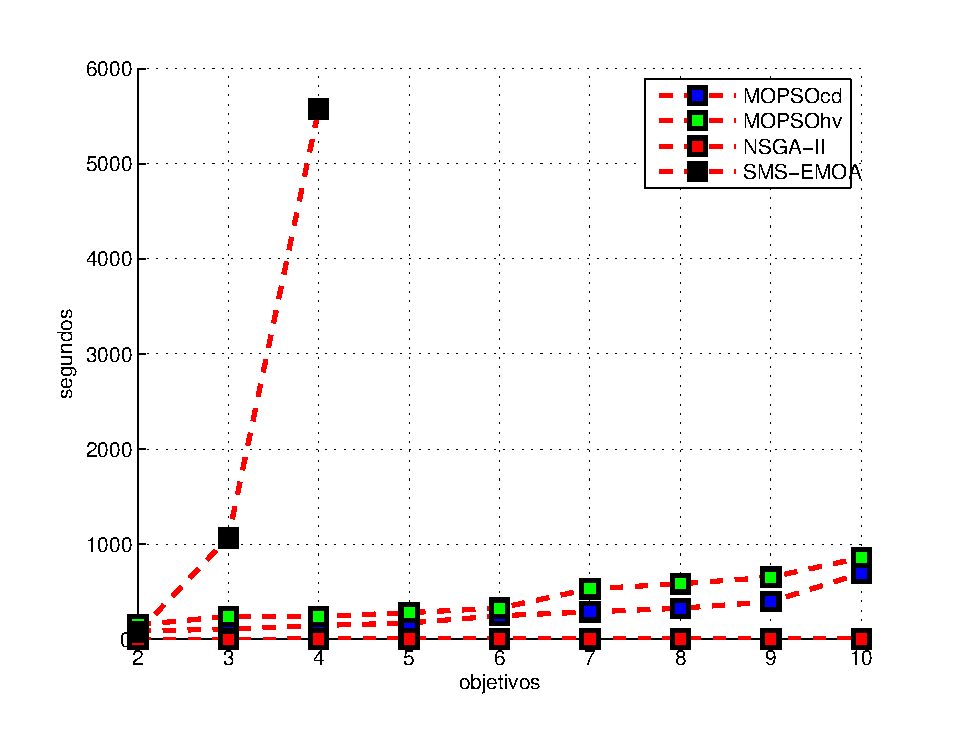
\includegraphics[scale=1]{Cap4/tiempoEscala.eps}
      \end{center}
	\caption[Tiempos en escalamiento para el problema DTLZ2.]{Resultados de tiempo en segundos aumentando el n\'umero de objetivos del problema DTLZ2.}
      \label{fig:tescala}
  \end{figure}

 